%
% $XORP: xorp/docs/user_manual/user_manual.tex,v 1.23 2008/12/24 22:06:50 jtc Exp $
%

\documentclass[11pt]{book}

%\usepackage[dvips]{changebar}

\usepackage{subfigure}
\usepackage{fullpage}
\usepackage{setspace}
\usepackage{times}
\usepackage{latexsym}
\usepackage{epsfig}
\usepackage{graphicx}
\usepackage{xspace}
\usepackage{color}
\usepackage{amsmath}
\usepackage{rotating}
\usepackage{moreverb}
\usepackage{listings}
\usepackage{alltt}
\usepackage{stmaryrd}
%\usepackage[dvipdf]{graphics}
%\usepackage[dvips]{graphicx}
%\usepackage{xorp}

\definecolor{gray}{rgb}{0.5,0.5,0.5}
\newcommand{\etc}{\emph{etc.}\xspace}
\newcommand{\ie}{\emph{i.e.,}\xspace}
\newcommand{\eg}{\emph{e.g.,}\xspace}
%\newcommand{\comment}[1]{{\color{gray}[\textsf{#1}]}}
%\newcommand{\comment}[1]{}

% Changebar stuff
% \newenvironment{colorcode}{\color{blue}}{}
% \renewcommand{\cbstart}{\begin{colorcode}}
% \renewcommand{\cbend}{\end{colorcode}}

% \pagestyle{empty}

\topmargin=0.0in
\textheight=9.0in
%\textwidth=7.0in

%
% Set style to not indent paragraphs, and to have a blank line between
% paragraphs.  While this style is not as elegant for prose as the
% defaults, it's more appropriate for manuals where there are lots of
% single line paragraphs.
%
\setlength{\parindent}{0pt} 
\setlength{\parskip}{0.5\baselineskip}
\setlength{\topsep}{0pt}
\setlength{\itemsep}{0pt}

%% Control the fonts and formatting used in the table of contents.
\usepackage[titles]{xorp_toc}
%% Aesthetic spacing redefines to cancel the effects of parskip
\setlength{\cftbeforechapskip}{2ex}
\setlength{\cftbeforesecskip}{-1.5ex}
\setlength{\cftbeforesubsecskip}{-1.5ex}
%% Use Helvetica-Narrow Bold for Chapter entries
\renewcommand{\cftchapfont}{%
  \fontsize{11}{13}\usefont{OT1}{phv}{bc}{n}\selectfont
}

\begin{document}

\title{{\Huge XORP User Manual}\\
\vspace{1ex}
Version 1.6-RC}
\author{ XORP, Inc.					\\
         {\it http://www.xorp.org/}			\\
	 {\it feedback@xorp.org}
}
\date{December 24, 2008}

\maketitle


%%%%%%%%%%%%%%%%%%%%%%%%%%%%%%%%%%%%%%%%%%%%%%%%%%%%%%%%%%%%%%%%%%%%%%%
%
% Local definitions
%
%\newcommand{\xorpsh}{\textsc{xorpsh}}
\newcommand{\xorp}{{\small XORP}\xspace}
\newcommand{\xorpsh}{{\sf\small xorpsh}\xspace}
\newcommand{\rtrmgr}{{\sf\small xorp\_rtrmgr}\xspace}
\newcommand{\stt}{\tt\small}
\newcommand{\ssf}{\sf\small}


%%%%%%%%%%%%%%%%%%%%%%%%%%%%%%%%%%%%%%%%%%%%%%%%%%%%%%%%%%%%%%%%%%%%%%%
%
% $XORP: xorp/docs/user_manual/preface.tex,v 1.10 2008/10/02 21:56:44 bms Exp $
%

\chapter*{Preface}

\vspace{-0.1in}
This User Manual describes the process of configuring and operating a
router running XORP.  At the time of writing, XORP is a
work-in-progress, and is evolving relatively quickly.  We hope this
user manual accurately reflects the functionality available in XORP,
but it is likely to date quite quickly.  An up-to-date copy of this
manual will always be available from {\it http://www.candelatech.com/xorp.ct/}.

\section*{Contributing to this Manual}
\vspace{-0.1in}
XORP is an open-source project, and this manual is an open-source
manual.  Like the XORP software, it is covered by the XORP license,
which permits you to modify it and use it for any purpose whatsoever,
so long as the copyright is preserved.  Please help us improve this
manual by sending contributions, suggestions, and criticism to {\it
  feedback@xorp.org}.

\section*{The XORP License}
\vspace{-0.3in}
\begin{alltt}
\small\noindent
\copyright 2004-2011 XORP, Inc and Others
\copyright 2004-2005 University College London

With the exception of code derived from other sources, all XORP software
is copyrighted by XORP, Inc. [Copyright (c) 2001-2011 XORP, Inc and Others].
Files containing derived software are listed in the "LICENSE.other" file
together with their corresponding copyrights and original licenses.

All XORP software is licensed under the GNU General Public License,
Version 2, June 1991 contained in the "LICENSE.gpl" file unless
otherwise indicated in the source file.

Software in source files that refer to the "LICENSE.lgpl" file is
licensed under the GNU Lesser General Public License, Version 2.1,
February 1999 contained in "LICENSE.lgpl".
\end{alltt}

Portions of the XORP CLI use modified version of the {\it libtecla}
library which is covered by the following license.

\section*{The Libtecla License}
\vspace{-0.3in}
\begin{alltt}
\small\noindent
Copyright (c) 2000, 2001 by Martin C. Shepherd.

All rights reserved.

Permission is hereby granted, free of charge, to any person obtaining a
copy of this software and associated documentation files (the
"Software"), to deal in the Software without restriction, including
without limitation the rights to use, copy, modify, merge, publish,
distribute, and/or sell copies of the Software, and to permit persons
to whom the Software is furnished to do so, provided that the above
copyright notice(s) and this permission notice appear in all copies of
the Software and that both the above copyright notice(s) and this
permission notice appear in supporting documentation.

THE SOFTWARE IS PROVIDED "AS IS", WITHOUT WARRANTY OF ANY KIND, EXPRESS
OR IMPLIED, INCLUDING BUT NOT LIMITED TO THE WARRANTIES OF
MERCHANTABILITY, FITNESS FOR A PARTICULAR PURPOSE AND NONINFRINGEMENT
OF THIRD PARTY RIGHTS. IN NO EVENT SHALL THE COPYRIGHT HOLDER OR
HOLDERS INCLUDED IN THIS NOTICE BE LIABLE FOR ANY CLAIM, OR ANY SPECIAL
INDIRECT OR CONSEQUENTIAL DAMAGES, OR ANY DAMAGES WHATSOEVER RESULTING
FROM LOSS OF USE, DATA OR PROFITS, WHETHER IN AN ACTION OF CONTRACT,
NEGLIGENCE OR OTHER TORTIOUS ACTION, ARISING OUT OF OR IN CONNECTION
WITH THE USE OR PERFORMANCE OF THIS SOFTWARE.

Except as contained in this notice, the name of a copyright holder
shall not be used in advertising or otherwise to promote the sale, use
or other dealings in this Software without prior written authorization
of the copyright holder.
\end{alltt}

\tableofcontents
%
% $XORP: xorp/docs/user_manual/glossary.tex,v 1.3 2005/04/07 03:05:33 pavlin Exp $
%

\chapter*{Glossary}
\begin{description}

  \item{\bf AS}: see Autonomous System.

  \item{\bf Autonomous System}: a routing domain that is under one
  administrative authority, and which implements its own routing
  policies.  Key concept in BGP.

  \item{\bf BGP}: Border Gateway Protocol.  See Chapter \ref{bgp}.

  \item{\bf Bootstrap Router}: A PIM-SM router that chooses the RPs for
  a domain from amongst a set of candidate RPs.

  \item{\bf BSR}: See Bootstrap Router.

  \item{\bf Candidate RP}: A PIM-SM router that is configured to be a
  candidate to be an RP.  The Bootstrap Router will then choose the
  RPs from the set of candidates.

  \item{\bf Dynamic Route}: A route learned from another router via a
  routing protocol such as RIP or BGP.

  \item{\bf EGP}: see Exterior Gateway Protocol.

  \item{\bf Exterior Gateway Protocol}: a routing protocol used to route
  between Autonomous Systems.  The main example is BGP.

  \item{\bf IGMP}: Internet Group Management Protocol.  See Chapter
  \ref{igmp}.

  \item{\bf IGP}: see Interior Gateway Protocol.

  \item{\bf Interior Gateway Protocol}: a routing protocol used to route
  within an Autonomous System.  Examples include RIP, OSPF and IS-IS.

  \item{\bf Live CD}: A CD-ROM that is bootable.  In the context of
  \xorp, the Live CD can be used to produce a low-cost router without
  needing to install any software.

  \item{\bf MLD}: Multicast Listener Discovery protocols.  See Chapter
  \ref{igmp}.

  \item{\bf MRIB}: See Multicast RIB.

  \item{\bf Multicast RIB}: the part of the RIB that holds multicast routes.
  These are not directly used for forwarding, but instead are used by
  multicast routing protocols such as PIM-SM to perform RPF checks
  when building the multicast distibution tree.

  \item{\bf OSPF}: See Open Shortest Path First.

  \item{\bf Open Shortest Path First:} an IGP routing protocol based on
  a link-state algorithm.  Used to route within medium to large
networks. See Chapter \ref{ospf}

  \item{\bf PIM-SM}: Protocol Independent Multicast, Sparse Mode. See
  Chapter \ref{pimsm}.

  \item{\bf Rendezvous Point}: A router used in PIM-SM as part of the
  rendezvous process by which new senders are grafted on to the
  multicast tree.

  \item{\bf Reverse Path Forwarding}: many multicast routing protocols
  such as PIM-SM build a multicast distribution tree based on the best
  route back from each receiver to the source, hence multicast packets
  will be forwarded along the reverse of the path to the source.

  \item{\bf RIB}: See Routing Information Base.

  \item{\bf RIP}: Routing Information Protocol.  See Chapter \ref{rip}.

  \item{\bf Routing Information Base}: the collection of routes learned
  from all the dynamic routing protocols running on the router.
  Subdivided into a Unicast RIB for unicast routes and a Multicast RIB.

  \item{\bf RP}: See Rendezvous Point.

  \item{\bf RPF}: See Reverse Path Forwarding.

  \item{\bf Static Route}: A route that has been manually configured on
  the router.

  \item{\bf xorpsh}: \xorp command shell.  See Chapter \ref{xorpsh}.

  \item{\bf xorp\_rtrmgr}: \xorp router manager process.  See Chapter
  \ref{xorpsh}.

\end{description}

%
% $XORP: xorp/docs/user_manual/cli_intro.tex,v 1.4 2005/04/07 03:04:15 pavlin Exp $
%

\chapter{Command Structure}
\label{xorpsh}

\section{Introduction}
To interact with a \xorp router using the command line interface (CLI),
the user runs the \xorp command shell ``\xorpsh''.  This allows
configuration of the router and monitoring of the router state.

In this chapter we describe how to interact with \xorpsh.  In later
chapters we describe the details of how to configure BGP, PIM, SNMP and
other processes.

The user interface style is loosely modelled on that of a Juniper
router.  This manual and the xorpsh itself are works in progress, and
so may change significantly in the future.

\section{Running xorpsh}
The \xorpsh command provides an interactive command shell to a \xorp user,
similar in many ways to the role played by a Unix shell.  In a production
router or on the \xorp LiveCD, \xorpsh might be set up as an user's
login shell - they would login to the router via ssh and be directly
in the \xorpsh environment.  However, for research and development
purposes, it makes more sense to login normally to the machine running
the \xorp processes, and to run \xorpsh directly from the Unix command
line.

\xorpsh should normally be run as a regular user; it is neither
necessary or desirable to run it as root.  If an user is to be
permitted to make changes to the running router configuration, that user
needs to be in the Unix group {\tt xorp}.  The choice of GID for group
{\tt xorp} is not important.

\xorpsh needs to be able to communicate with the \xorp router
management process \rtrmgr using the local file system.  If
the \rtrmgr cannot write files in /tmp that \xorpsh can read, then
\xorpsh will not be able to authenticate the user to the \rtrmgr.

Multiple users can run \xorpsh simultaneously.  There is some degree of
configuration locking to prevent simultaneous changes to the router
configuration, but currently this is fairly primitive.

To facilitate automated \xorp router configuration, it is possible to use
\xorpsh in non-interactive mode (\eg as part of a shell script).
This is described in details in Section~\ref{xorpsh:non-interactive-mode}.

\newpage
\section{Basic Commands}

On starting \xorpsh, you will be presented with a command line prompt:
\vspace{0.1in}

\noindent\framebox[\textwidth][l]{
\begin{minipage}{\textwidth}
\begin{alltt}
Xorp>
\end{alltt}
\end{minipage}
}
\vspace{0.1in}

\noindent
You can exit \xorpsh at any time by trying Control-d.

\noindent
Typing ``?'' at the prompt will list the commands currently available to
you:
\vspace{0.1in}

\noindent\framebox[\textwidth][l]{
\begin{minipage}[l]{\textwidth}
\begin{alltt}
\begin{tabbing}
Xorp> \textbf{?}\\
Po\=ssible compl\=etions:\\
\>configure       \>Switch to configuration mode\\
\>help            \>Provide help with commands\\
\>quit            \>Quit this command session\\
\>show            \>Display information about the system
\end{tabbing}
\end{alltt}
\end{minipage}
}
\vspace{0.1in}

\noindent
If you type the first letter or letters of a command, and hit
{\tt <Tab>}, then command completion will occur.

\noindent
At any time you can type ``?'' again to see further 
command completions.  For
example:
\vspace{0.1in}

\noindent\framebox[\textwidth][l]{
\begin{minipage}{\textwidth}
\begin{alltt}
\begin{tabbing}
Xorp> \textbf{config?}\\
Po\=ssible compl\=etions:\\
\>configure\>Switch to configuration mode\\
Xorp> \textbf{config}
\end{tabbing}
\end{alltt}
\end{minipage}
}
\vspace{0.1in}

\noindent
If the cursor is after the command, typing ``?'' will list the possible
parameters for the command:
\vspace{0.1in}

\noindent\framebox[\textwidth][l]{
\begin{minipage}{4in}
\begin{alltt}
\begin{tabbing}
Xorp> \textbf{configure ?}\\
Po\=ssible compl\=etions:\\
\><[Enter]>       \>Execute this command\\
\>exclusive       \>Switch to configuration mode, locking out other users\\
Xorp> \textbf{configure}
\end{tabbing}
\end{alltt}
\end{minipage}
}

\newpage
\subsection{Command History and Command Line Editing}

\xorpsh supports emacs-style command history and editing of the text
on the command line.  The most important commands are:
\begin{itemize}
\item The {\bf up-arrow} or {\bf control-p} moves to the previous
command in the history.
\item The {\bf down-arrow} or {\bf control-n} moves to the next
command in the history.
\item The {\bf left-arrow} or {\bf control-b} moves back along the
command line.
\item The {\bf right-arrow} or {\bf control-f} move forward along the
command line.
\item {\bf control-a} moves to the beginning of the command line.
\item {\bf control-e} moves to the end of the command line.
\item {\bf control-d} deletes the character directly under the cursor.
\item {\bf control-t} toggles (swaps) the character under the cursor with
the character immediately preceding it.
\item {\bf control-space} marks the current cursor position.
\item {\bf control-w} deletes the text between the mark and the current
cursor position, copying the deleted text to the cut buffer.
\item {\bf control-k} kills (deletes) from the cursor to the end of the
command line, copying the deleted text to the cut buffer.
\item {\bf control-y} yanks (pastes) the text from the cut buffer,
inserting it at the
current cursor location.
\end{itemize}

\newpage
\section{Command Modes}

\xorpsh has two command modes:
\begin{description}
\item{\bf Operational Mode,}  which allows interaction with the router
to monitor its operation and status.
\item{\bf Configuration Mode,} which allows the user to view the
configuration of the router, to change that configuration, and to
load and save configurations to file.
\end{description}
Generally speaking, operational mode is considered to give
non-privileged access; there should be nothing an user can type that
would seriously impact the operation of the router.  In contrast,
configuration mode allows all aspects of router operation to be
modified.

In the long run, \xorpsh and the \rtrmgr will probably come to support
fine-grained access control, so that some users can be given
permission to change only subsets of the router configuration.  At the
present time though, there is no fine-grained access control.

An user can only enter configuration mode if that user is in the {\tt xorp}
Unix group.

\section{Operational Mode}
\noindent\framebox[\textwidth][l]{
\begin{minipage}{6in}
\begin{alltt}
\begin{tabbing}
Xorp> \textbf{?}\\
Po\=ssible compl\=etions:\\
\>configure       \>Switch to configuration mode\\
\>help            \>Provide help with commands\\
\>quit            \>Quit this command session\\
\>show            \>Display information about the system
\end{tabbing}
\end{alltt}
\end{minipage}
}
\vspace{0.1in}

The main commands in operational mode are:
\begin{description}
\item{\bf configure}: switches from operational mode to configuration
mode.
\item{\bf help}: provides online help.
\item{\bf quit}: quit from xorpsh.
\item{\bf show}: displays many aspects of the running state of the
router.
\end{description}

\newpage
\subsection{Show Command}
\noindent\framebox[\textwidth][l]{
\begin{minipage}{6in}
\begin{alltt}
\begin{tabbing}
Xorp> \textbf{show ?}\\
Po\=ssible compl\=etions:\\
\>  <[Enter]>       \>Execute this command\\
\>  bgp             \>Display information about BGP\\
\>  host            \>Display information about the host\\
\>  igmp            \>Display information about IGMP\\
\>  interfaces      \>Show network interface information\\
\>  mfea            \>Display information about IPv4 MFEA\\
\>  mfea6           \>Display information about IPv6 MFEA\\
\>  mld             \>Display information about MLD\\
\>  pim             \>Display information about IPv4 PIM\\
\>  pim6            \>Display information about IPv6 PIM\\
\>  rip             \>Display information about RIP\\
\>  route           \>Show route table\\
Xorp> \textbf{show}
\end{tabbing}
\end{alltt}
\end{minipage}
}
\vspace{0.1in}

\noindent
The \emph{show} command is used to display many aspects of the running state
of the router.  We don't describe the sub-commands here, because they
depend on the running state of the router.  For example, only a router
that is running BGP should provide {\tt show bgp} commands.

As an example, we show the peers of a BGP router:
\vspace{0.1in}

\noindent\framebox[\textwidth][l]{
\begin{minipage}{6in}
\begin{alltt}
\begin{tabbing}
Xorp> \textbf{show bgp peers detail}\\
OK\\
Pe\=er 1: local 192.150.187.108/179 remote 192.150.187.109/179\\
\>  Peer ID: 192.150.187.109\\
\>  Peer State: ESTABLISHED\\
\>  Admin State: START\\
\>  Negotiated BGP Version: 4\\
\>  Peer AS Number: 65000\\
\>  Updates Received: 5157,  Updates Sent: 0\\
\>  Messages Received: 5159,  Messages Sent: 1\\
\>  Time since last received update: 4 seconds\\
\>  Number of transitions to ESTABLISHED: 1\\
\>  Time since last entering ESTABLISHED state: 47 seconds\\
\>  Retry Interval: 120 seconds\\
\>  Hold Time: 90 seconds,  Keep Alive Time: 30 seconds\\
\>  Configured Hold Time: 90 seconds,  Configured Keep Alive Time: 30 seconds\\
\>  Minimum AS Origination Interval: 0 seconds\\
\>  Minimum Route Advertisement Interval: 0 seconds\\
\end{tabbing}
\end{alltt}
\end{minipage}
}
\vspace{0.1in}

\newpage
\section{Configuration Mode}
\noindent\framebox[\textwidth][l]{
\begin{minipage}{6in}
\begin{alltt}
\begin{tabbing}
Xorp> \textbf{configure}\\
Entering configuration mode.\\
There are no other users in configuration mode.\\
\noindent[edit]\\
XORP>
\end{tabbing}
\end{alltt}
\end{minipage}
}
\vspace{0.1in}

\noindent
When in configuration mode, the command prompt changes to be all
capitals.
The command prompt is also usually preceded by a line indicating which
part of the configuration tree is currently being edited.
\vspace{0.1in}

\noindent\framebox[\textwidth][l]{
\begin{minipage}{6in}
\begin{alltt}
\begin{tabbing}
[edit]\\
XORP> \textbf{?}\\
Po\=ssible completi\=ons:\\
\>  create          \>Create a sub-element\\
\>  delete          \>Delete a configuration element\\
\>  edit            \>Edit a sub-element\\
\>  exit            \>Exit from this configuration level\\
\>  help            \>Provide help with commands\\
\>  load            \>Load configuration from a file\\
\>  quit            \>Quit from this level\\
\>  run             \>Run an operational-mode command\\
\>  save            \>Save configuration to a file\\
\>  set             \>Set the value of a parameter\\
\>  show            \>Show the value of a parameter\\
\>  top             \>Exit to top level of configuration\\
\>  up              \>Exit one level of configuration\\
XORP> 
\end{tabbing}
\end{alltt}
\end{minipage}
}
\vspace{0.1in}

\newpage
\noindent
The router configuration has a tree form similar to the directory
structure on a Unix filesystem.  The current configuration or parts of
the configuration can be
shown with the \emph{show} command:
\vspace{0.1in}

\noindent\framebox[\textwidth][l]{
\begin{minipage}{6in}
\begin{alltt}
\begin{tabbing}
xx\=xx\=xx\=xx\=xx\=\kill
[edit]\\
XORP> \textbf{show interfaces}\\
\>interface rl0 \{\\
\>\>description: "control interface"\\
\>\>vif rl0 \{\\
\>\>\>address 192.150.187.108 \{\\
\>\>\>\>prefix-length: 25\\
\>\>\>\>broadcast: 192.150.187.255\\
\>\>\>\>disable: false\\
\>\>\>\}\\
\>\>\>disable: false\\
\>\>\}\\
\>\>disable: false\\
\>\}\\
\>targetname: "fea"\\
\end{tabbing}
\end{alltt}
\end{minipage}
}
\vspace{0.1in}

\newpage
\subsection{Moving around the Configuration Tree}
You can change the current location in the configuration tree using
the \emph{edit}, \emph{exit}, \emph{quit}, \emph{top} and \emph{up} commands.
\begin{itemize}
\item \textbf{edit $<$\textit{element name}$>$}:       Edit a sub-element
\item \textbf{exit}:       Exit from this configuration level, or if
at top level, exit configuration mode.
\item \textbf{quit}:       Quit from this level
\item \textbf{top}:        Exit to top level of configuration
\item \textbf{up}:         Exit one level of configuration
\end{itemize}

\noindent
For example:
\vspace{0.1in}

\noindent\framebox[\textwidth][l]{
\begin{minipage}{6in}
\begin{alltt}
\begin{tabbing}
xx\=xx\=xx\=xx\=xx\=\kill
[edit]\\
XORP> \textbf{edit interfaces interface rl0 vif rl0}\\
\noindent[edit interfaces interface rl0 vif rl0]\\
XORP> \textbf{show}\\
\>address 192.150.187.108 \{\\
\>\>prefix-length: 25\\
\>\>broadcast: 192.150.187.255\\
\>\>disable: false\\
\>\}\\
\>disable: false\\
\\
\noindent[edit interfaces interface rl0 vif rl0]\\
XORP> \textbf{up}\\
\noindent[edit interfaces interface rl0]\\
XORP> \textbf{top}\\
\noindent[edit]\\
XORP>
\end{tabbing}
\end{alltt}
\end{minipage}
}

\subsection{Loading and Saving Configurations}

On startup, the \rtrmgr will read a configuration file.  It will then
start up and configure the various router components as specified in
the configuration file.

The configuration file can be created externally, using a normal text
editor, or it can be saved from the running router configuration.  A
configuration file can also be loaded into a running router, causing
the previous running configuration to be discarded.  The commands for
this are:
\begin{itemize}
\item \textbf{save $<$\textit{filename}$>$}: save the current
configuration in the specified file.
\item \textbf{load $<$\textit{filename}$>$}: load the specified file,
discarding the currently running configuration.
\end{itemize}

\subsection{Setting Configuration Values}

\begin{itemize}
\item \textbf{set $<$\textit{path to config}$>$
$<$\textit{value}$>$}: set the value of the specified configuration
node.
\end{itemize}
The \emph{set} command is used to set or change the value of a configuration
option.  The change does not actually take effect immediately - the
\emph{commit} command must be used to apply this and any other uncommitted
changes.

In the example below, the prefix length (netmask) of address
192.150.187.108 on vif rl0 is changed, but not yet committed.  The
``{\tt >}'' indicates parts of the configuration that have changed but
not yet been committed.
\vspace{0.1in}

\noindent\framebox[\textwidth][l]{
\begin{minipage}{6in}
\begin{alltt}
\begin{tabbing}
xx\=xx\=xx\=xx\=xx\=\kill
\noindent[edit interfaces interface rl0]\\
XORP> \textbf{show}\\
\>description: "control interface"\\
\>vif rl0 \{\\
\>\>address 192.150.187.108 \{\\
\>\>\>prefix-length: 25\\
\>\>\>broadcast: 192.150.187.255\\
\>\>\>disable: false\\
\>\>\}\\
\>\>disable: false\\
\>\}\\
\>disable: false\\
\\
\noindent[edit interfaces interface rl0]\\
XORP> \textbf{set vif rl0 address 192.150.187.108 prefix-length 24}\\
OK\\
\\
\noindent[edit interfaces interface rl0]\\
XORP> \textbf{show}\\
\>description: "control interface"\\
\>vif rl0 \{\\
\>\>address 192.150.187.108 \{\\
>\>\>\>prefix-length: 24\\
\>\>\>broadcast: 192.150.187.255\\
\>\>\>disable: false\\
\>\>\}\\
\>\>disable: false\\
\>\}\\
\end{tabbing}
\end{alltt}
\end{minipage}
}

\newpage
\subsection{Adding New Configuration}
\begin{itemize}

\item \textbf{create $<$\textit{path to new config node}$>$}
: create new configuration node.
\item \textbf{create $<$\textit{path to new config node}$>$ \{}
: create new configuration node and start editing it.

\end{itemize}

New configuration can be added by the \emph{create} command.
If we type \emph{create} followed by the path to a new configuration node,
the node will be created. All parameters within that node will be assigned
their default values (if exist). After that the node can be edited with the
\emph{edit} command.
If we type \emph{\{} after the path to the new configuration node,
the node will be created, the default values will be assigned, and we can
directly start editing that node.
The user interface for this is currently rather
primitive and doesn't permit the more free-form configuration allowed
in configuration files.

\newpage
For example, to configure a second vif on interface rl0:
\vspace{0.1in}

\noindent\framebox[\textwidth][l]{
\begin{minipage}{6in}
\begin{alltt}
\begin{tabbing}
xx\=xx\=xx\=xx\=xx\=\kill
\noindent[edit interfaces interface rl0]\\
XORP> \textbf{show}\\
\>description: "control interface"\\
\>vif rl0 \{\\
\>\>address 192.150.187.108 \{\\
\>\>\>prefix-length: 24\\
\>\>\>broadcast: 192.150.187.255\\
\>\>\>disable: false\\
\>\>\}\\
\>\>disable: false\\
\>\}\\
\>disable: false\\
\\
\noindent[edit interfaces interface rl0]\\
XORP> \textbf{create vif rl0b \{}\\
\>\>>\> \textbf{address 10.0.0.1 \{}\\
\>\>>\>\> \textbf{prefix-length 16}\\
\>\>>\>\> \textbf{broadcast 10.0.255.255}\\
\>\>>\>\> \textbf{disable false}\\
\>\>>\>\> \textbf{\}}\\
\>\>>\> \textbf{disable false}\\
\>\>>\> \textbf{\}}\\
\noindent[edit interfaces interface rl0]\\
XORP> \textbf{show}\\
\>description: "control interface"\\
\>vif rl0 \{\\
\>\>address 192.150.187.108 \{\\
\>\>\>prefix-length: 24\\
\>\>\>broadcast: 192.150.187.255\\
\>\>\>disable: false\\
\>\>\}\\
\>\>disable: false\\
\>\}\\
> vif rl0b \{\\
>\>\> address 10.0.0.1 \{\\
>\>\>\> prefix-length: 16\\
>\>\>\> broadcast: 10.0.255.255\\
>\>\>\> disable: false\\
>\>\>\}\\
>\>\>disable: false\\
>\>\}\\
\>disable: false\\
\end{tabbing}
\end{alltt}
\end{minipage}
}

\subsection{Deleting Parts of the Configuration}

The \emph{delete} command can be used to delete subtrees from the
configuration.  The deletion will be visible in the results of the
\emph{show} command, but will not actually take place until the changes are
committed.
\vspace{0.1in}

\noindent\framebox[\textwidth][l]{
\begin{minipage}{6in}
\begin{alltt}
\begin{tabbing}
xx\=xx\=xx\=xx\=xx\=\kill
XORP> \textbf{show interfaces interface rl0}\\
\>description: "control interface"\\
\>vif rl0 \{\\
\>\>address 192.150.187.108 \{\\
\>\>\>prefix-length: 24\\
\>\>\>broadcast: 192.150.187.255\\
\>\>\>disable: false\\
\>\>\}\\
\>\>disable: false\\
\>\}\\
\>vif rl0b \{\\
\>\> address 10.0.0.1 \{\\
\>\>\> prefix-length: 16\\
\>\>\> broadcast: 10.0.255.255\\
\>\>\> disable: false\\
\>\>\}\\
\>\>disable: false\\
\>\}\\
\>disable: false\\
\\
\noindent[edit]\\
XORP> \textbf{delete interfaces interface rl0 vif rl0b}\\
Deleting:\\
\>address 10.0.0.1 \{\\
\>\>prefix-length: 16\\
\>\>broadcast: 10.0.255.255\\
\>\>disable: false\\
\>\}\\
\\
OK\\
\noindent[edit]\\
XORP> \textbf{show interfaces interface rl0}\\
\>description: "control interface"\\
\>vif rl0 \{\\
\>\>address 192.150.187.108 \{\\
\>\>\>prefix-length: 24\\
\>\>\>broadcast: 192.150.187.255\\
\>\>\>disable: false\\
\>\>\}\\
\>\>disable: false\\
\>\}\\
\>disable: false
\end{tabbing}
\end{alltt}
\end{minipage}
}

\newpage
\subsection{Committing Changes}

\noindent\framebox[\textwidth][l]{
\begin{minipage}{6in}
\begin{alltt}
\begin{tabbing}
\noindent[edit interfaces interface rl0]\\
XORP> \textbf{commit}\\
OK
\end{tabbing}
\end{alltt}
\end{minipage}
}
\vspace{0.1in}

The \emph{commit} command commits all the current configuration changes.
This can take a number of seconds before the response is given.

{\it If xorpsh was built with debugging enabled, the response can be
considerably more verbose than shown above!}

If two or more users are logged in using configuration mode, and one
of them changes the configuration, the others will receive a warning:
\vspace{0.1in}

\noindent\framebox[\textwidth][l]{
\begin{minipage}{6in}
\begin{alltt}
\begin{tabbing}
\noindent[edit]\\
XORP>\\
The configuration had been changed by user mjh\\
XORP>
\end{tabbing}
\end{alltt}
\end{minipage}
}
\vspace{0.1in}


\subsection{Discarding Changes}

The user can discard a batch of changes by editing them back to their
original configuration, or by using the \emph{exit} command to leave
configuration mode:
\vspace{0.1in}

\noindent\framebox[\textwidth][l]{
\begin{minipage}{6in}
\begin{alltt}
\begin{tabbing}
\noindent[edit]\\
XORP> \textbf{exit}\\
ERROR: There are uncommitted changes\\
Use "commit" to commit the changes, or "exit discard" to discard them\\
XORP> \textbf{exit discard}\\
Xorp>
\end{tabbing}
\end{alltt}
\end{minipage}
}
\vspace{0.1in}


\section{Running xorpsh in Non-Interactive Mode}
\label{xorpsh:non-interactive-mode}

Typically \xorpsh would be used as an interactive command shell.
However, it is possible to use \xorpsh in non-interactive mode
(\eg as part of a shell script). This could be useful for automated
XORP router configuration such as adding new network interfaces
to the XORP configuration for new PPP dial-up clients.

The following non-interactive modes are supported:

\begin{itemize}

  \item Running \xorpsh as part of UNIX command-line pipes:

\begin{verbatim}
echo "show host os" | ./xorpsh
cat filename | ./xorpsh
./xorpsh < filename
\end{verbatim}

  \item Running \xorpsh as part of a shell script:

\begin{verbatim}
#!/bin/sh

./xorpsh <<!
show host os
!
\end{verbatim}

  \item Running commands that are supplied by the ``-c'' \xorpsh
   command-line option:

\begin{verbatim}
./xorpsh -c "show host os"
\end{verbatim}

  \item Running \xorpsh as part of an ``expect'' script:

\begin{verbatim}
#!/usr/bin/env python
import time
import sys
import pexpect

child=pexpect.spawn ('./xorpsh')
child.expect('Xorp> ')
child.sendline('show host os | no-more')
child.sendeof()
while 1:
        line = child.readline()
        if not line:
                break
        print line,
child.close()
\end{verbatim}

Note that if \xorpsh is run in non-interactive more as part of an ``expect''
script where there is a TTY associated with the \xorpsh process, then
\xorpsh may use the internal pager if the output from a command is very long.
In that case, it is advisable that the internal pager is explicitly disabled
by using the ``no-more'' pipe as in the above example.

\end{itemize}


%
% $XORP: xorp/docs/user_manual/config_overview.tex,v 1.12 2005/06/01 00:39:10 pavlin Exp $
%

\chapter{Configuration Overview}
\section{Introduction}

A XORP router must be configured to perform the desired operations.
The configuration information can be provided in one of the two ways:

\begin{itemize}
\item
  Use a configuration file when the rtrmgr is started.
  By default, the rtrmgr will load the configuration from file
  ``config.boot'' in the XORP installation directory.
  This file can be specified by the ``-b~~$<$filename$>$'' command line
  option:
\begin{verbatim}
    xorp_rtrmgr -b my_config.boot
\end{verbatim}

    See ``rtrmgr/config.boot.sample'' for an example of a
    configuration file (note that this file MUST be modified
    before using it).

\item
  Use the xorpsh command line interface after the rtrmgr is started.
  It should be noted that command line completion in the xorpsh
  does greatly simplify configuration.
\end{itemize}

\noindent
A mixture of both methods is permissible. For example,
a configuration file can also be loaded from within the xorpsh.

At very minimum, a router's interfaces must be configured (see
Section~\ref{sec:network_interfaces}). Typically, the FEA needs to be
configured (\eg to enable unicast forwarding); the FEA configuration is
described in Section~\ref{sec:fea}. All protocol configuration is
described in Section~\ref{sec:protocols}.

\section{Network Interfaces}
\label{sec:network_interfaces}

A XORP router will only use interfaces that it has been explicitly
configured to use. Even for protocols such as BGP that are agnostic to
interfaces, if the next-hop router for a routing entry is not through
a configured interface the route will not be installed. For protocols
that are explicitly aware of interfaces only configured interfaces
will be used.

Every physical network device in the system is considered to be an
``interface''. Every interface can contain a number of virtual
interfaces (``vif''s). In the majority of cases the interface name and
vif name will be identical and will map to the name given to the
interface by the operating system. A virtual interface is configured
with the address or addresses that should be used. At each level in
the configuration hierarchy ({\tt interface}, {\tt vif} and
{\tt address}) it is necessary to enable this part of the
configuration.

\vspace{0.1in}
\noindent\framebox[\textwidth][l]{\scriptsize
\begin{minipage}{6in}
\begin{alltt}
\begin{tabbing}
xx\=xx\=xx\=xx\=xx\=\kill
interfaces \{\\
\>interface dc0 \{\\
\>\>description: "data interface"\\
\>\>disable: false\\
\>\>/* default-system-config */\\
\>\>vif dc0 \{\\
\>\>\>disable: false\\
\>\>\>address 10.10.10.10 \{\\
\>\>\>\>prefix-length: 24\\
\>\>\>\>broadcast: 10.10.10.255\\
\>\>\>\>disable: false\\
\>\>\>\}\\
\>\>\>/*\\
\>\>\>address 10:10:10:10:10:10:10:10 \{\\
\>\>\>\>prefix-length: 64\\
\>\>\>\>disable: false\\
\>\>\>\}\\
\>\>\>*/\\
\>\>\}\\
\>\}\\
\}
\end{tabbing}
\end{alltt}
\end{minipage}
}
\vspace{0.1in}

We recommend that you select the interfaces that you want to use on
your system and configure them as above. If you are configuring an
interface that is currently being used by the the system make sure
that there is no mismatch in the {\tt address}, {\tt prefix-length} and
{\tt broadcast} arguments.
If the \linebreak
{\tt default-system-config} statement is used, it
instructs the FEA that the interface should be configured by using
the existing interface information from the underlying system.
In that case, the {\tt vif} and {\tt address} sections must not be
configured.

\section{Forwarding Engine Abstraction}
\label{sec:fea}

It is a requirement to explicitly enable forwarding for each
protocol family.

\vspace{0.1in}
\noindent\framebox[\textwidth][l]{\scriptsize
\begin{minipage}{6in}
\begin{alltt}
\begin{tabbing}
xx\=xx\=xx\=xx\=xx\=\kill
fea \{\\
\>unicast-forwarding4 \{\\
\>\>disable: false\\
\>\}\\
/*\\
\>unicast-forwarding6 \{\\
\>\>disable: false\\
\>\}\\
*/\\
\}
\end{tabbing}
\end{alltt}
\end{minipage}
}
\vspace{0.1in}

If IPv4 forwarding is required you will require the configuration
above. If the system supports IPv6 and IPv6 forwarding is required,
then the {\tt unicast-forwarding6} statement must be used to enable
it~\footnote{Note that prior to XORP Release-1.1, the
{\tt enable-unicast-forwarding4} and {\tt enable-unicast-forwarding6}
flags were used instead to enable or disable the IPv4 and IPv6 forwarding.}.

\newpage
\section{Protocols}
\label{sec:protocols}

A unicast router typically will be configured with one or more
of the following protocols:
StaticRoutes (Section~\ref{sec:protocols:static_routes}),
RIP (Section~\ref{sec:protocols:rip})
or BGP (Section~\ref{sec:protocols:bgp}).

A multicast router must have the MFEA configured
(Section~\ref{sec:protocols:mfea}). Typically, a multicast router should
have IGMP/MLD configured (Section~\ref{sec:protocols:mld6igmp}).
Currently, PIM-SM is the only multicast routing protocol implemented
(Section~\ref{sec:protocols:pim}). If some multicast-specific static
routes need to be installed in the MRIB (for computing the reverse-path
forwarding information), those can be specified in the StaticRoutes
configuration (Section~\ref{sec:protocols:static_routes}).
If there are no
unicast routing protocols configured, the FIB2MRIB module may
need to be configured as well (Section~\ref{sec:protocols:fib2mrib}).

\subsection{Static Routes}
\label{sec:protocols:static_routes}

This is the simplest routing protocol in XORP. It allows the
installation of unicast or multicast static routes (either IPv4 or
IPv6).  Note that in case of multicast the routes are installed only
in the user-level Multicast Routing Information Base and are used for
multicast-specific reverse-path forwarding information by multicast routing
protocols such as PIM-SM.

\vspace{0.1in}
\noindent\framebox[\textwidth][l]{\scriptsize
\begin{minipage}{6in}
\begin{alltt}
\begin{tabbing}
xx\=xx\=xx\=xx\=xx\=\kill
protocols \{\\
\>static \{\\
\>\>route4 10.20.0.0/16 \{\\
\>\>\>nexthop: 10.10.10.20\\
\>\>\>metric: 1\\
\>\>\}\\
\>\>mrib-route4 10.20.0.0/16 \{\\
\>\>\>nexthop: 10.10.10.30\\
\>\>\>metric: 1\\
\>\>\}\\
\>\>/*\\
\>\>route6 20:20:20:20::/64 \{\\
\>\>\>nexthop: 10:10:10:10:10:10:10:20\\
\>\>\>metric: 1\\
\>\>\}\\
\>\>mrib-route6 20:20:20:20::/64 \{\\
\>\>\>nexthop: 10:10:10:10:10:10:10:30\\
\>\>\>metric: 1\\
\>\>\}\\
\>\>*/\\
\>\}\\
\}
\end{tabbing}
\end{alltt}
\end{minipage}
}
\vspace{0.1in}

\newpage
\subsection{Routing Information Protocol}
\label{sec:protocols:rip}

In order to run RIP it is sufficient to specify the set of interfaces,
vifs and addresses ({\tt interface}, {\tt vif} and {\tt address}) on
which RIP is enabled~\footnote{Note that prior to XORP Release-1.1,
the {\tt enable} flag was used instead of {\tt disable} to enable
or disable each part of the configuration.}.

If you wish to announce routes then it is necessary to
{\tt export}~\footnote{Note that in release candidate 1.0-RC, the {\tt import}
 keyword is used in place of {\tt export}.}
the routes that are to be announced. For example, {\tt connected},
{\tt static} and {\tt rip}.

{\bf Note that this mechanism for originating
routes is temporary. In the next release it will be replaced by
a more generic policy framework. Unfortunately, the same keyword
{\stt export} will be used but with different syntax.}

\vspace{0.1in}
\noindent\framebox[\textwidth][l]{\scriptsize
\begin{minipage}{6in}
\begin{alltt}
\begin{tabbing}
xx\=xx\=xx\=xx\=xx\=\kill
protocols \{\\
\>rip \{\\
\>/* Redistribute routes for connected interfaces */\\
\>\>/*\\
\>\>export connected \{\\
\>\>\>metric: 0\\
\>\>\>tag: 0\\
\>\>\}\\
\>\>*/\\
\>/* Redistribute static routes */\\
\>\>/*\\
\>\>export static \{\\
\>\>\>metric: 1\\
\>\>\>tag: 0\\
\>\>\}\\
\>\>*/\\
\>/* Run on specified network interface addresses */\\
\>/*\\
\>\>interface dc0 \{\\
\>\>\>vif dc0 \{\\
\>\>\>\>address 10.10.10.10 \{\\
\>\>\>\>\>disable: false\\
\>\>\>\>\}\\
\>\>\>\}\\
\>\>\}\\
\>*/\\
\>\}\\
\}
\end{tabbing}
\end{alltt}
\end{minipage}
}

\newpage
\subsection{Border Gateway Protocol}
\label{sec:protocols:bgp}

In order to run BGP the {\tt bgp-id} (BGP Identifier) and {\tt local-as}
(Autonomous System number) must be specified.

The {\tt peer} statement specifies a peering. The argument to the peer
statement is the IP address of the peer. The {\tt local-ip} is the IP
address that TCP should use. The {\tt as} is the Autonomous System Number
of the peer.

\vspace{0.1in}
\noindent\framebox[\textwidth][l]{\scriptsize
\begin{minipage}{6in}
\begin{alltt}
\begin{tabbing}
xx\=xx\=xx\=xx\=xx\=\kill
protocols \{\\
\>bgp \{\\
\>\>bgp-id: 10.10.10.10\\
\>\>local-as: 65002\\
\\
\>\>peer 10.30.30.30 \{\\
\>\>\>local-ip: 10.10.10.10\\
\>\>\>as: 65000\\
\>\>\>next-hop: 10.10.10.20\\
\>\>\>/*\\
\>\>\>local-port: 179\\
\>\>\>peer-port: 179\\
\>\>\>*/\\
\>\>\>/* holdtime: 120 */\\
\>\>\>/* disable: false */\\
\\
\>\>\>/* IPv4 unicast is enabled by default */\\
\>\>\>/* ipv4-unicast: true */\\
\\
\>\>\>/* Optionally enable other AFI/SAFI combinations */\\
\>\>\>/* ipv4-multicast: true */\\
\>\>\>/* ipv6-unicast: true */\\
\>\>\>/* ipv6-multicast: true */\\
\>\>\}\\
\\
\>\>/* Originate IPv4 Routes */\\
\>\>/*\\
\>\>network4 10.10.10.0/24 \{\\
\>\>\>next-hop: 10.10.10.10\\
\>\>\>unicast: true\\
\>\>\>multicast: true\\
\>\>\}\\
\>\>*/\\
\\
\>\>/* Originate IPv6 Routes */\\
\>\>/*\\
\>\>network6 10:10:10:10::/64 \{\\
\>\>\>next-hop: 10:10:10:10:10:10:10:10\\
\>\>\>unicast: true\\
\>\>\>multicast: true\\
\>\>\}\\
\>\>*/\\
\>\}\\
\}
\end{tabbing}
\end{alltt}
\end{minipage}
}
\vspace{0.1in}

Currently BGP is not able to {\tt import} routes from other routing
protocols such as {\tt static}. It is however possible to originate routes
using {\tt network4} and {\tt network6} statements such as in the above
example.

\newpage
\subsection{Multicast Forwarding Engine Abstraction}
\label{sec:protocols:mfea}

The MFEA must be configured if the XORP router is to be used for multicast
routing. The MFEA for IPv4 and IPv6 are configured separately.

In the configuration we must explicitly configure the entity itself, and
each {\tt vif}. The {\tt traceoptions} section is used to explicitly enable
log information that can be used for debugging purpose~\footnote{Note that
prior to XORP Release-1.1, the {\tt enable} flag was used instead of
{\tt disable} to enable or disable each part of the configuration.}.

\vspace{0.1in}
\noindent\framebox[\textwidth][l]{\scriptsize
\begin{minipage}{6in}
\begin{alltt}
\begin{tabbing}
xx\=xx\=xx\=xx\=xx\=\kill
plumbing \{\\
\>mfea4 \{\\
\>\>disable: false\\
\>\>interface dc0 \{\\
\>\>\>vif dc0 \{\\
\>\>\>\>disable: false\\
\>\>\>\}\\
\>\>\}\\
\>\>interface register\_vif \{\\
\>\>\>vif register\_vif \{\\
\>\>\>\>/* Note: this vif should be always enabled */\\
\>\>\>\>disable: true\\
\>\>\>\}\\
\>\>\}\\
\>\>traceoptions \{\\
\>\>\>flag all \{\\
\>\>\>\>disable: true\\
\>\>\>\}\\
\>\>\}\\
\>\}\\
\}\\
\\
plumbing \{\\
\>mfea6 \{\\
\>\>disable: true\\
\>\>interface dc0 \{\\
\>\>\>vif dc0 \{\\
\>\>\>\>disable: true\\
\>\>\>\}\\
\>\>\}\\
\>\>interface register\_vif \{\\
\>\>\>vif register\_vif \{\\
\>\>\>\>/* Note: this vif should be always enabled */\\
\>\>\>\>disable: true\\
\>\>\>\}\\
\>\>\}\\
\>\>traceoptions \{\\
\>\>\>flag all \{\\
\>\>\>\>disable: true\\
\>\>\>\}\\
\>\>\}\\
\>\}\\
\}
\end{tabbing}
\end{alltt}
\end{minipage}
}
\vspace{0.1in}

Note that the interface/vif named {\tt register\_vif} is special.
If PIM-SM is configured, then 
\linebreak
{\tt register\_vif} must be enabled
in the MFEA.

\newpage
\subsection{Internet Group Management Protocol/Multicast Listener Discovery}
\label{sec:protocols:mld6igmp}

IGMP/MLD should be configured if the XORP router is to be used for multicast
routing and if we want to track multicast group membership for directly
connected subnets. Typically this is the case for a multicast router,
therefore it should be enabled. IGMP and MLD are configured separately:
IGMP is used for tracking IPv4 multicast members; MLD is used for tracking
IPv6 multicast members.

In the configuration we must explicitly configure each entity and
each {\tt vif}. The {\tt traceoptions} section is used to explicitly
enable log information that can be used for debugging purpose~\footnote{Note
that prior to XORP Release-1.1, the {\tt enable} flag was used instead of
{\tt disable} to enable or disable each part of the configuration.}.

\vspace{0.1in}
\noindent\framebox[\textwidth][l]{\scriptsize
\begin{minipage}{6in}
\begin{alltt}
\begin{tabbing}
xx\=xx\=xx\=xx\=xx\=\kill
protocols \{\\
\>igmp \{\\
\>\>disable: false\\
\>\>interface dc0 \{\\
\>\>\>vif dc0 \{\\
\>\>\>\>disable: false\\
\>\>\>\>/* version: 2 */\\
\>\>\>\>/* enable-ip-router-alert-option-check: false */\\
\>\>\>\>/* query-interval: 125 */\\
\>\>\>\>/* query-last-member-interval: 1 */\\
\>\>\>\>/* query-response-interval: 10 */\\
\>\>\>\>/* robust-count: 2 */\\
\>\>\>\}\\
\>\>\}\\
\>\>traceoptions \{\\
\>\>\>flag all \{\\
\>\>\>\>disable: false\\
\>\>\>\}\\
\>\>\}\\
\>\}\\
\}\\
\\
protocols \{\\
\>mld \{\\
\>\>disable: false\\
\>\>interface dc0 \{\\
\>\>\>vif dc0 \{\\
\>\>\>\>disable: false\\
\>\>\>\>/* version: 1 */\\
\>\>\>\>/* enable-ip-router-alert-option-check: false */\\
\>\>\>\>/* query-interval: 125 */\\
\>\>\>\>/* query-last-member-interval: 1 */\\
\>\>\>\>/* query-response-interval: 10 */\\
\>\>\>\>/* robust-count: 2 */\\
\>\>\>\}\\
\>\>\}\\
\>\>traceoptions \{\\
\>\>\>flag all \{\\
\>\>\>\>disable: false\\
\>\>\>\}\\
\>\>\}\\
\>\}\\
\}
\end{tabbing}
\end{alltt}
\end{minipage}
}
\vspace{0.1in}

A number of parameters have default values, therefore
they don't have to be configured (those parameters are commented-out
in the above sample configuration).

The {\tt version} parameter is used to configure the MLD/IGMP protocol
version per virtual interface~\footnote{Note that the {\tt version}
statement appeared after XORP Release-1.1.}.

The {\tt enable-ip-router-alert-option-check} parameter is used to
enable the IP Router Alert option check per virtual interface~\footnote{Note
that the {\tt enable-ip-router-alert-option-check} statement appeared after
XORP Release-1.1.}.

The {\tt query-interval} parameter is used to configure (per virtual
interface) the interval (in seconds) between general queries sent by the
querier~\footnote{Note that the {\tt query-interval} statement appeared
after XORP Release-1.1.}.

The {\tt query-last-member-interval} parameter is used to configure (per
virtual interface) the maximum response time (in seconds) inserted into
group-specific queries sent in response to leave group messages. It is
also the interval between group-specific query messages~\footnote{Note
that the {\tt query-last-member-interval} statement appeared after XORP
Release-1.1.}.

The {\tt query-response-interval} parameter is used to configure (per
virtual interface) the maximum response time (in seconds) inserted into
the periodic general queries~\footnote{Note that the {\tt
query-response-interval} statement appeared after XORP Release-1.1.}.

The {\tt robust-count} parameter is used to configure the robustness
variable count that allows tuning for the expected packet loss on a
subnet~\footnote{Note that the {\tt robust-count} statement appeared
after XORP Release-1.1.}.


\newpage
\subsection{Protocol Independent Multicast - Sparse Mode}
\label{sec:protocols:pim}

PIM-SM should be configured if the XORP router is to be used for
multicast routing in PIM-SM domain. PIM-SM for IPv4 and IPv6 are
configured separately. At minimum, the entity itself and the
virtual interfaces should be enabled, and the mechanism for obtaining
the Candidate-RP set (either the Bootstrap mechanism, or a static-RP
set)~\footnote{Note that prior to XORP Release-1.1, the {\tt enable} flag
was used instead of {\tt disable} to enable or disable each part of the
configuration.}.

\vspace{0.1in}
\noindent\framebox[\textwidth][l]{\scriptsize
\begin{minipage}{4.5in}
\begin{alltt}
\begin{tabbing}
xx\=xx\=xx\=xx\=xx\=\kill
protocols \{\\
\>pimsm4 \{\\
\>\>disable: false\\
\>\>interface dc0 \{\\
\>\>\>vif dc0 \{\\
\>\>\>\>disable: false\\
\>\>\>\>/* enable-ip-router-alert-option-check: false */\\
\>\>\>\>/* dr-priority: 1 */\\
\>\>\>\>/* hello-period: 30 */\\
\>\>\>\>/* hello-triggered-delay: 5 */\\
\>\>\>\>/* alternative-subnet 10.40.0.0/16 */\\
\>\>\>\}\\
\>\>\}\\
\>\>interface register\_vif \{\\
\>\>\>vif register\_vif \{\\
\>\>\>\>/* Note: this vif should be always enabled */\\
\>\>\>\>disable: false\\
\>\>\>\}\\
\>\>\}\\
\\
\>\>static-rps \{\\
\>\>\>rp 10.60.0.1 \{\\
\>\>\>\>group-prefix 224.0.0.0/4 \{\\
\>\>\>\>\>/* rp-priority: 192 */\\
\>\>\>\>\>/* hash-mask-len: 30 */\\
\>\>\>\>\}\\
\>\>\>\}\\
\>\>\}\\
\\
\>\>bootstrap \{\\
\>\>\>disable: false\\
\>\>\>cand-bsr \{\\
\>\>\>\>scope-zone 224.0.0.0/4 \{\\
\>\>\>\>\>/* is-scope-zone: false */\\
\>\>\>\>\>cand-bsr-by-vif-name: "dc0"\\
\>\>\>\>\>/* cand-bsr-by-vif-addr: 10.10.10.10 */\\
\>\>\>\>\>/* bsr-priority: 1 */\\
\>\>\>\>\>/* hash-mask-len: 30 */\\
\>\>\>\>\}\\
\>\>\>\}\\
\\
\>\>\>cand-rp \{\\
\>\>\>\>group-prefix 224.0.0.0/4 \{\\
\>\>\>\>\>/* is-scope-zone: false */\\
\>\>\>\>\>cand-rp-by-vif-name: "dc0"\\
\>\>\>\>\>/* cand-rp-by-vif-addr: 10.10.10.10 */\\
\>\>\>\>\>/* rp-priority: 192 */\\
\>\>\>\>\>/* rp-holdtime: 150 */\\
\>\>\>\>\}\\
\>\>\>\}\\
\>\>\}\\
\\
{\rm continued overleaf....}
\end{tabbing}
\end{alltt}
\end{minipage}
}
\newpage
\vspace{0.1in}
\noindent\framebox[\textwidth][l]{\scriptsize
\begin{minipage}{4.5in}
\begin{alltt}
\begin{tabbing}
xx\=xx\=xx\=xx\=xx\=\kill
\>\>switch-to-spt-threshold \{\\
\>\>\>/* approx. 1K bytes/s (10Kbps) threshold */\\
\>\>\>disable: false\\
\>\>\>interval-sec: 100\\
\>\>\>bytes: 102400\\
\>\>\}\\
\\
\>\>traceoptions \{\\
\>\>\>flag all \{\\
\>\>\>\>disable: false\\
\>\>\>\}\\
\>\>\}\\
\>\}\\
\}
\\
\\
protocols \{\\
\>pimsm6 \{\\
\>\>disable: false\\
\>\>interface dc0 \{\\
\>\>\>vif dc0 \{\\
\>\>\>\>disable: false\\
\>\>\>\>/* enable-ip-router-alert-option-check: false */\\
\>\>\>\>/* dr-priority: 1 */\\
\>\>\>\>/* hello-period: 30 */\\
\>\>\>\>/* hello-triggered-delay: 5 */\\
\>\>\>\>/* alternative-subnet 40:40:40:40::/64 */\\
\>\>\>\}\\
\>\>\}\\
\>\>interface register\_vif \{\\
\>\>\>vif register\_vif \{\\
\>\>\>\>/* Note: this vif should be always enabled */\\
\>\>\>\>disable: false\\
\>\>\>\}\\
\>\>\}\\
\\
\>\>static-rps \{\\
\>\>\>rp 50:50:50:50:50:50:50:50 \{\\
\>\>\>\>group-prefix ff00::/8 \{\\
\>\>\>\>\>/* rp-priority: 192 */\\
\>\>\>\>\>/* hash-mask-len: 126 */\\
\>\>\>\>\}\\
\>\>\>\}\\
\>\>\}\\
\\
\>\>bootstrap \{\\
\>\>\>disable: false\\
\>\>\>cand-bsr \{\\
\>\>\>\>scope-zone ff00::/8 \{\\
\>\>\>\>\>/* is-scope-zone: false */\\
\>\>\>\>\>cand-bsr-by-vif-name: "dc0"\\
\>\>\>\>\>/* cand-bsr-by-vif-addr: 10:10:10:10:10:10:10:10 */\\
\>\>\>\>\>/* bsr-priority: 1 */\\
\>\>\>\>\>/* hash-mask-len: 126 */\\
\>\>\>\>\}\\
\>\>\>\}\\
\\
\>\>\>cand-rp \{\\
\>\>\>\>group-prefix ff00::/8 \{\\
\>\>\>\>\>/* is-scope-zone: false */\\
\>\>\>\>\>cand-rp-by-vif-name: "dc0"\\
\>\>\>\>\>/* cand-rp-by-vif-addr: 10:10:10:10:10:10:10:10 */\\
\>\>\>\>\>/* rp-priority: 192 */\\
\>\>\>\>\>/* rp-holdtime: 150 */\\
\>\>\>\>\}\\
\>\>\>\}\\
\>\>\}\\
\\
{\rm continued overleaf....}
\end{tabbing}
\end{alltt}
\end{minipage}
}
\newpage
\vspace{0.1in}
\noindent\framebox[\textwidth][l]{\scriptsize
\begin{minipage}{4.5in}
\begin{alltt}
\begin{tabbing}
xx\=xx\=xx\=xx\=xx\=\kill
\>\>switch-to-spt-threshold \{\\
\>\>\>/* approx. 1K bytes/s (10Kbps) threshold */\\
\>\>\>disable: false\\
\>\>\>interval-sec: 100\\
\>\>\>bytes: 102400\\
\>\>\}\\
\\
\>\>traceoptions \{\\
\>\>\>flag all \{\\
\>\>\>\>disable: false\\
\>\>\>\}\\
\>\>\}\\
\>\}\\
\}
\end{tabbing}
\end{alltt}
\end{minipage}
}
\vspace{0.1in}

A number of parameters have default values, therefore
they don't have to be configured (those parameters are commented-out
in the above sample configuration).

Note that the interface/vif named {\tt register\_vif} is special.
If PIM-SM is configured, then {\tt register\_vif} must be enabled.

The {\tt enable-ip-router-alert-option-check} parameter is used to
enable the IP Router Alert option check per virtual interface~\footnote{Note
that the {\tt enable-ip-router-alert-option-check} statement appeared after
XORP Release-1.1.}.

The {\tt dr-priority} parameter is used to configure the Designated Router
priority per virtual interface (note that in case of {\tt register\_vif}
it is not used).

The {\tt hello-period} parameter is used to configure the PIM Hello
messages period (in seconds) per virtual interface~\footnote{Note that the
{\tt hello-period} statement appeared after XORP Release-1.1.}. It must
be an integer between 1 and 18724.

The {\tt hello-triggered-delay} parameter is used to configure the
randomized triggered delay of the PIM Hello messages (in
seconds) per virtual interface~\footnote{Note that the
{\tt hello-triggered-delay} statement appeared after XORP
Release-1.1.}. It must be an integer between 1 and 255.

The {\tt alternative-subnet} statement is used to associate additional
subnets with a network interface. For example, if you want to make
incoming traffic with a non-local source address appear as it is
coming from a local subnet, then {\tt alternative-subnet} can be
used. Typically, this is needed as a work-around solution when we use
uni-directional interfaces for receiving traffic (e.g., satellite
links).  Note: use {\tt alternative-subnet} with extreme care, only if
you know what you are really doing!

If PIM-SM uses static RPs, those can be configured within the
{\tt static-rps} section. For each RP, an {\tt rp} section is needed, and each
section should contain the multicast prefix address the static RP is
configured with. The RP priority can be modified with the {\tt rp-priority}
parameter.

If PIM-SM uses the Bootstrap mechanism to obtain the Candidate-RP set,
this can be configured in the {\tt bootstrap} section.
If the XORP router is to be used as a Candidate-BSR, this should be
specified in the {\tt cand-bsr} section.
For a router to be a Candidate-BSR it must advertise for
each zone (scoped or non-scoped) the associated multicast prefix address.
The {\tt cand-bsr} section should contain {\tt scope-zone} statements for each
multicast prefix address.
The vif name with the address that is to be used as the Candidate-BSR
is specified by the {\tt cand-bsr-by-vif-name} statement.
The particular vif's address can be specified by the
{\tt cand-bsr-by-vif-addr} statement. If the
{\tt cand-bsr-by-vif-addr} statement is omitted, a domain-wide
address (if exists) that belongs to that interface is chosen by the router
itself~\footnote{Note that the {\tt cand-bsr-by-vif-addr} statement
appeared after XORP Release-1.1.}.
The Candidate-BSR priority can be modified with the {\tt bsr-priority}
parameter.

If the XORP router is to be a Candidate-RP, this should be specified
in the {\tt cand-rp} section.
For a router to be a Candidate-RP it must advertise for
each zone (scoped or non-scoped) the associated multicast prefix address.
The {\tt cand-rp} section should contain {\tt group-prefix} statements
for each multicast prefix address.
The vif name with the address that is to be used as the Candidate-RP
is specified by the {\tt cand-rp-by-vif-name} statement.
The particular vif's address can be specified by the
{\tt cand-rp-by-vif-addr} statement. If the
{\tt cand-rp-by-vif-addr} statement is omitted, a domain-wide
address (if exists) that belongs to that interface is chosen by the router
itself~\footnote{Note that the {\tt cand-rp-by-vif-addr} statement
appeared after XORP Release-1.1.}.
The Candidate-RP priority can be modified with the
{\tt rp-priority} parameter; the Candidate-RP holdtime can be modified
with the {\tt rp-holdtime} parameter.

The {\tt is-scope-zone} parameter is used to specify whether a
Candidate-BSR {\tt scope-zone} or a Candidate-RP {\tt group-prefix} is
scoped. Currently, 
scoped zones are not well tested, hence it is recommended {\tt scope-zone}
is always set to {\tt false}.
Note that typically the {\tt hash-mask-len} should not be modified; if you
don't know what {\tt hash-mask-len} is used for, don't modify it!

The {\tt switch-to-spt-threshold} section can be used to specify the
multicast data bandwidth threshold used by the last-hop PIM-SM routers
and the RPs to initiate shortest-path switch toward the multicast source.
Parameter {\tt interval-sec} is used to specify the periodic measurement
interval;
parameter {\tt bytes} is used to specify the threshold in number of bytes
within the measurement interval. It is recommended that the measurement
interval is not too small, and should be on the order of tens of seconds.

The {\tt traceoptions} section is used to explicitly enable log information
that can be used for debugging purpose.

\newpage
\subsection{FIB2MRIB}
\label{sec:protocols:fib2mrib}

The FIB2MRIB module is used to obtain the Forwarding Information Base
information from the underlying system (via the FEA), and to propagate
it to the MRIB, so it can be used by multicast routing protocols
such as PIM-SM. Typically, it is needed only if the unicast routing
protocols (if any) on that router do not inject routes into the
MRIB~\footnote{Note that prior to XORP Release-1.1, the {\tt enable} flag
was used instead of {\tt disable} to enable or disable each part of the
configuration.}.

\vspace{0.1in}
\noindent\framebox[\textwidth][l]{\scriptsize
\begin{minipage}{6in}
\begin{alltt}
\begin{tabbing}
xx\=xx\=xx\=xx\=xx\=\kill
protocols \{\\
\>fib2mrib \{\\
\>\>disable: false\\
\>\}\\
\}
\end{tabbing}
\end{alltt}
\end{minipage}
}
\vspace{0.1in}



\chapter{Network Interfaces}

\section{Terminology and Concepts}

vif vs interface, v4, v6

\section{Configuring Network Interfaces}

A XORP router will only use interfaces that it has been explicitly
configured to use. Even for protocols such as BGP that are agnostic to
interfaces, if the next-hop router for a routing entry is not through
a configured interface the route will not be installed. For protocols
such as RIP that are explicitly aware of interfaces only, configured
interfaces will be used.

Every physical network device in the system is considered to be an
``interface''. Thus an ethernet interface or an ATM adaptor might be
considered to be an interface.  

Every interface can contain a number of virtual interfaces (``VIF''s).
In many cases there will be a one-to-one correspondence between
interfaces and VIFs, but this does not have to be the case.  In the
case of ethernet, the same physical interface might have multiple
logical devices in the form of VLANs.  Such VLANs would be multiple
vifs on a single interface.\footnote{As of the 1.0 release, VLANs are
not yet supported in XORP.}

In cases where the interface only supports one VIF, the VIF name will
be the same as the interface name, and will map to the name given to
the interface by the operating system.   A virtual interface is
configured with the address or addresses that should be used. At each
level in the configuration hierarchy ({\tt interface}, {\tt vif} and
{\tt address}) it is necessary to enable this part of the
configuration.

\subsection{Configuration Syntax}

The available configuration syntax for network interfaces and
addresses is as follows:

\vspace{0.1in}
\noindent\framebox[\textwidth][l]{\scriptsize
\begin{minipage}{6in}
\begin{alltt}
\begin{tabbing}
xx\=xx\=xx\=xx\=xx\=\kill
interfaces \{\\
\>interface {\it text} \{\\
\>\>description: {\it text}\\
\>\>mac: {\it macaddr}\\
\>\>mtu: {\it uint}\\
\>\>default-system-config\\
\>\>enabled: {\it bool}\\
\>\>vif {\it text} \{\\
\>\>\>enabled: {\it bool}\\
\>\>\>address {\it IPv4-addr} \{\\
\>\>\>\>prefix-length: {\it int(1..32}\\
\>\>\>\>broadcast: {\it IPv4-addr}\\
\>\>\>\>destination: {\it IPv4-addr}\\
\>\>\>\>enabled: {\it bool}\\
\>\>\>\}\\
\>\>\>address {\it IPv6-addr} \{\\
\>\>\>\>prefix-length: {\it int(1..128)}\\
\>\>\>\>destination: {\it IPv6-addr}\\
\>\>\>\>enabled: {\it bool}\\
\>\>\>\}\\
\>\>\}\\
\>\}\\
\}
\end{tabbing}
\end{alltt}
\end{minipage}
}

\subsection{Example Configurations}

We recommend that you select the interfaces that you want to use on
your system and configure them as below. If you are configuring an
interface that is currently being used by the the system make sure
that there is no mismatch in the {\tt address}, {\tt prefix-length} and
{\tt broadcast} arguments.

\vspace{0.1in}
\noindent\framebox[\textwidth][l]{\scriptsize
\begin{minipage}{6in}
\begin{alltt}
\begin{tabbing}
xx\=xx\=xx\=xx\=xx\=\kill
interfaces \{\\
\>interface dc0 \{\\
\>\>description: "data interface"\\
\>\>enabled: true\\
\>\>vif dc0 \{\\
\>\>\>enabled: true\\
\>\>\>address 10.10.10.10 \{\\
\>\>\>\>prefix-length: 24\\
\>\>\>\>broadcast: 10.10.10.255\\
\>\>\>\>enabled: true\\
\>\>\>\}\\
\>\>\>\\
\>\>\>address 10:10:10:10:10:10:10:10 \{\\
\>\>\>\>prefix-length: 64\\
\>\>\>\>enabled: true\\
\>\>\>\}\\
\>\>\>\\
\>\>\}\\
\>\}\\
\}
\end{tabbing}
\end{alltt}
\end{minipage}
}

If the {\tt default-system-config} statement is used, it instructs the
FEA that the interface should be configured by using the existing
interface information from the underlying system.  In that case, the
{\tt vif} and {\tt address} sections must not be configured.

\vspace{0.1in}
\noindent\framebox[\textwidth][l]{\scriptsize
\begin{minipage}{6in}
\begin{alltt}
\begin{tabbing}
xx\=xx\=xx\=xx\=xx\=\kill
interfaces \{\\
\>interface dc0 \{\\
\>\>description: "data interface"\\
\>\>enabled: true\\
\>\>default-system-config\\
\>\}\\
\}
\end{tabbing}
\end{alltt}
\end{minipage}
}
\vspace{0.1in}



\section{Monitoring Network Interfaces}

description of op-mode commands
%
% $XORP$
%

\chapter{Firewall}
\label{firewall}
\section{Firewall Terminology and Concepts}

For security purposes, a router can be configured to inspect the
forwarded network traffic and take certain actions. Those actions are
based on a set of rules called ``firewall rules''. Each firewall rule
has a matching criteria (\eg source and destination address), and an
action. Typical actions are to allow or deny the forwarding of the
packets that match the rule.



\newpage
\section{Configuring Firewall Rules}

Firewall configuration can contain many rules.
The rules are evaluated in certain order for each incoming packet.
In XORP the configuration rules are numbered, and rules with smaller
number are evaluated first. On certain systems (\eg FreeBSD) the largest
rule number is limited by the system to 65534~\footnote{On FreeBSD with
{\tt ipfw} enabled, rule number 65535 is reserved by the system as the
default rule that matches all packets and it cannot be modified or
deleted.}, therefore the XORP  configuration shouldn't include rule
numbers that are larger.

Currently (July 2008), firewall configuration is supported only for
*BSD and Linux~\footnote{See file ERRATA from the XORP distribution for
additional information how to compile XORP on Linux with firewall
support enabled.}.

\subsection{Configuration Syntax}

The available configuration syntax for firewall rules is as
follows~\footnote{Currently (July 2008) XORP has only preliminary support to
  configure firewall rules.}: 

\vspace{0.1in}
\noindent\framebox[\textwidth][l]{\scriptsize
\begin{minipage}{6in}
\begin{alltt}
\begin{tabbing}
xx\=xx\=xx\=xx\=xx\=\kill
firewall \{\\
\>rule4 {\it int(1..65534)} \{\\
\>\>action: {\it text}\\
\>\>protocol: {\it int(0..255)}\\
\>\>source \{\\
\>\>\>interface: {\it text}\\
\>\>\>vif: {\it text}\\
\>\>\>network: {\it IPv4}/{\it int(0..32)}\\
\>\>\>port-begin: {\it int(0..65535)}\\
\>\>\>port-end: {\it int(0..65535)}\\
\>\>\}\\
\>\>destination \{\\
\>\>\>network: {\it IPv4}/{\it int(0..32)}\\
\>\>\>port-begin: {\it int(0..65535)}\\
\>\>\>port-end: {\it int(0..65535)}\\
\>\>\}\\
\>\}\\
\>rule6 {\it int(1..65534)} \{\\
\>\>action: {\it text}\\
\>\>protocol: {\it int(0..255)}\\
\>\>source \{\\
\>\>\>interface: {\it text}\\
\>\>\>vif: {\it text}\\
\>\>\>network: {\it IPv6}/{\it int(0..128)}\\
\>\>\>port-begin: {\it int(0..65535)}\\
\>\>\>port-end: {\it int(0..65535)}\\
\>\>\}\\
\>\>destination \{\\
\>\>\>network: {\it IPv6}/{\it int(0..128)}\\
\>\>\>port-begin: {\it int(0..65535)}\\
\>\>\>port-end: {\it int(0..65535)}\\
\>\>\}\\
\>\}\\
\}
\end{tabbing}
\end{alltt}
\end{minipage}
}

\begin{description}
\item{\tt firewall}: this delimits all the firewall configuration
  information within the XORP configuration file.

\item{\tt rule4}: this delimits the configuration of a particular
  IPv4 firewall rule. The parameter is the rule number and must be
  in the interval [1..65534].

  For each IPv4 rule, the following configuration is possible:

\begin{description}

\item{\tt action}: this is the action that should be applied on packets
  that match the rule. It is a string with one of the following values:
\begin{itemize}
  \item {\tt none}: No action. Continue the evaluation with the next
  rule.
  \item {\tt pass}: Pass the matching packets.
  \item {\tt drop}: Drop the matching packets.
  \item {\tt reject}: Reject the matching packets (\ie drop them and try
  to send back the appropriate ICMP unreachable notice). Note that some
  systems don't support this mechanism; on such systems {\tt reject} is
  equivalent to {\tt drop}.
\end{itemize}

  This field is mandatory.

\item{\tt protocol}: this field specifies the IP protocol number as
  defined by IANA~\cite{IANA}, and is an integer value in the interval
  [0..255]. For example, TCP protocol number is 6, and UDP protocol
  number is 17. If it is set to 0 (the default value), all protocols are
  matched.

\item{\tt source}: this delimits the configuration of the matching
  criteria the is related to the source of the packet:
\begin{description}
\item{\tt interface}: this parameter is the name of the interface
  the packet arrives on. Only packets arriving on that interface will
  pass this criteria. The value mist be either the name of an interface
  known to the router forwarding path or an empty string (\ie any
  interface). The default value is an empty string.
\item{\tt vif}: this parameter is the name of the vif on the
  corresponding {\tt interface} the packet arrives on. Only packets
  arriving on that vif will pass this criteria. The value mist be either
  the name of a vif that belongs to {\tt interface} and is known to the
  router forwarding path or an empty string (\ie any interface). The
  default value is an empty string.
\item{\tt network}: this parameter specifies the source network address
  prefix. The value is in the form of an IP address and prefix-length in
  the {\it address/prefix-length} format. Only packets with source
  address that belong to this address prefix will pass this criteria.
  The default value is 0.0.0.0/0, \ie any source address.
\item{\tt port-begin}: this parameter specifies the lower bound of the
  source port number interval, and is an integer value in the interval
  [0..65535]. It applies only for TCP and UDP packets.
  Only packets with source port number that is equal or larger than
  {\tt port-begin} will pass this criteria. In other words, the source
  port number must be in the interval
  [{\tt port-begin}..{\tt port-end}]. The default value is 0.
\item{\tt port-end}: this parameter specifies the upper bound of the
  source port number interval, and is an integer value in the interval
  [0..65535]. It applies only for TCP and UDP packets.
  Only packets with source port number that is equal or smaller than
  {\tt port-end} will pass this criteria. In other words, the source
  port number must be in the interval
  [{\tt port-begin}..{\tt port-end}]. The default value is 65535.
\end{description}

\item{\tt destination}: this delimits the configuration of the matching
  criteria the is related to the destination of the packet:
\begin{description}
\item{\tt network}: this parameter specifies the destination network address
  prefix. The value is in the form of an IP address and prefix-length in
  the {\it address/prefix-length} format. Only packets with destination
  address that belong to this address prefix will pass this criteria.
  The default value is 0.0.0.0/0, \ie any destination address.
\item{\tt port-begin}: this parameter specifies the lower bound of the
  destination port number interval, and is an integer value in the interval
  [0..65535]. It applies only for TCP and UDP packets.
  Only packets with destination port number that is equal or larger than
  {\tt port-begin} will pass this criteria. In other words, the destination
  port number must be in the interval
  [{\tt port-begin}..{\tt port-end}]. The default value is 0.
\item{\tt port-end}: this parameter specifies the upper bound of the
  destination port number interval, and is an integer value in the interval
  [0..65535]. It applies only for TCP and UDP packets.
  Only packets with destination port number that is equal or smaller than
  {\tt port-end} will pass this criteria. In other words, the destination
  port number must be in the interval
  [{\tt port-begin}..{\tt port-end}]. The default value is 65535.
\end{description}

\end{description}

\item{\tt rule6}: this delimits the configuration of a particular
  IPv6 firewall rule. The parameter is the rule number and must be
  in the interval [1..65534].

  The IPv6 rule configuration is similar to the IPv4 configuration,
  except that IPv6 addresses are used instead of IPv4 addresses (where
  applicable).

  Note that on certain systems (\eg FreeBSD-7.0 with {\tt ipfw}) the
  firewall rule numbers for IPv4 and IPv6 use same number
  space. Therefore, the {\tt rule4} and {\tt rule6} rule numbers in the
  XORP configuration should also be chosen from the same number space.

\end{description}

\newpage
\subsection{Example Configurations}

We recommend that the initial firewall configuration uses rule numbers
with large interval between (\eg 100, 200, 300), such that other rules
can be inserted later if necessary.

\vspace{0.1in}
\noindent\framebox[\textwidth][l]{\scriptsize
\begin{minipage}{6in}
\begin{alltt}
\begin{tabbing}
xx\=xx\=xx\=xx\=xx\=\kill
firewall \{\\
\>rule4 100 \{\\
\>\>action: "pass"\\
\>\>protocol: 6 /* TCP */\\
\>\>destination \{\\
\>\>\>network: 10.10.10.10/32\\
\>\>\>port-begin: 80\\
\>\>\>port-end: 80\\
\>\>\}\\
\>\}\\
\>rule4 200 \{\\
\>\>action: "drop"\\
\>\>protocol: 6 /* TCP */\\
\>\>source \{\\
\>\>\>interface: "fxp0"\\
\>\>\>vif: "fxp0"\\
\>\>\>network: 0.0.0.0/0\\
\>\>\>port-begin: 0\\
\>\>\>port-end: 65535\\
\>\>\}\\
\>\>destination \{\\
\>\>\>network: 10.10.0.0/24\\
\>\>\>port-begin: 0\\
\>\>\>port-end: 1024\\
\>\>\}\\
\>\}\\
\>rule4 65000 \{\\
\>\>action: "pass"\\
\>\>protocol: 6 /* TCP */\\
\>\}\\
\}
\end{tabbing}
\end{alltt}
\end{minipage}
}

\vspace{0.1in}
In the example above, the router has only three firewall rules
configured. The first rule (rule 100) will allow all TCP traffic to IP
address 10.10.10.10 and TCP port number 80 (\ie HTTP requests) to pass.
The second rule (rule 200) will drop all TCP traffic arriving on
interface/vif {\tt fxp0/fxp0} if the destination IP address belongs to
subnet 10.10.0.0/24 and the destination TCP port number is in the
interval [0..1024].
The third rule (rule 65000) will allow all remaining TCP traffic.


\newpage
\section{Monitoring Firewall Rules}

Examples of firewall monitoring include displaying the set of installed
firewall rules in the data forwarding plane, or displaying information
about the number of packets that have matched a particular firewall
rule.

Currently (July 2008) XORP doesn't support monitoring firewall rules.
The commands that are provided with the underlying system should be used
to monitor the firewall rules (\eg {\tt ipfw} for FreeBSD and
{\tt iptables} for Linux).

\chapter{Forwarding Engine}

\section{Terminology and Concepts}

The forwarding engine is that part of a router that receives packets
and forwards then from one interface to another.  In the case of XORP,
the forwarding engine may be the kernel forwarding path on Linux or
FreeBSD, or it may reside in external forwarding hardware.  

On any particular router, it might be desirable to enable or disable
different parts of the forwarding functionality.  For example, a
router might only be intended to forward IPv6 packets but not IPv4
packets, or it might be intended to forward unicast packets but not
multicast packets.    Thus XORP provides the ability to enable and
configure various forwarding functionality.

In XORP, the term ``{\stt fea}'' refers to {\it Forwarding Engine
Abstraction} and the term ``{\stt mfea}'' refers to {\it Multicast
Forwarding Engine Abstraction}.  The term abstraction here refers to a
high-level configuration interface that should be the same
irrespective of whether the forwarding engine is provided in software
in the operating system kernel or in external forwarding hardware.

\newpage
\section{Configuration of the Forwarding Engine}

On a XORP router, forwarding functionality must be explicitly enabled
or no packets will be forwarded.  Forwarding can be separately enabled
for unicast and multicast, and for IPv4 and IPv6.  In addition,
multicast interfaces/vifs need to be explicitly enabled individually,
and certain special-purpose forwarding functionality can also be
enabled for multicast.

\subsection{Configuration Syntax}
\vspace{0.1in}
\noindent\framebox[\textwidth][l]{\scriptsize
\begin{minipage}{6in}
\begin{alltt}
\begin{tabbing}
xx\=xx\=xx\=xx\=xx\=\kill
fea \{\\
\>targetname: {\it txt}\\
\>enable-unicast-forwarding4: {\it bool}\\
\>enable-unicast-forwarding6: {\it bool}\\
\}
\\
plumbing \{\\
\>mfea4 \{\\
\>\>enabled: {\it bool}\\
\>\>interface {\it text} \{\\
\>\>\>vif {\it text} \{\\
\>\>\>\>enabled: {\it bool}\\
\>\>\>\}\\
\>\>\}\\
\>\>interface register\_vif \{\\
\>\>\>vif register\_vif \{\\
\>\>\>\>enabled: {\it bool}\\
\>\>\>\}\\
\>\>\}\\
\>\>traceoptions \{\\
\>\>\>flag all \{\\
\>\>\>\>enabled: {\it bool}\\
\>\>\>\}\\
\>\>\}\\
\>\}\\
\\
\>mfea6 \{\\
\>\>enabled: {\it bool}\\
\>\>interface {\it text} \{\\
\>\>\>vif {\it text} \{\\
\>\>\>\>enabled: {\it bool}\\
\>\>\>\}\\
\>\>\}\\
\>\>interface register\_vif \{\\
\>\>\>vif register\_vif \{\\
\>\>\>\>enabled: {\it bool}\\
\>\>\>\}\\
\>\>\}\\
\>\>traceoptions \{\\
\>\>\>flag \{\\
\>\>\>\>all \{\\
\>\>\>\>\>enabled: {\it bool}\\
\>\>\>\>\}\\
\>\>\>\}\\
\>\>\}\\
\>\}\\
\}
\end{tabbing}
\end{alltt}
\end{minipage}
}
\vspace{0.1in}

\begin{description}
\item{\stt fea}: this delimits the configuration for the unicast
  forwarding engine functionality. 

  The following unicast forwarding engine parameters can be configured:
\begin{description}
\item{\tt targetname} this is the name for this instance of the
  forwarding engine abstraction.  It defaults to ``{\stt fea}'', and
  it is strongly recommended that this default is {\it not} overridden
  under normal usage scenarios.
\item{\stt enable-unicast-forwarding4}: this takes the value {\stt
  true} or {\stt false}, and determines whether the router will
  forward unicast IPv4 packets.
\item{\stt enable-unicast-forwarding6}: this takes the value {\stt
  true} or {\stt false}, and determines whether the router will
  forward unicast IPv4 packets.
\end{description}
\item{\stt plumbing}: this delimits a part of the router configuration
  used for the plumbing together of packet forwarding functionality.
  Multicast forwarding configuration must be part of this grouping.
\item{\stt mfea4}: this delimits the part of the router configuration
  related to multicast forwarding of IPv4 packets.

  The following multicast forwarding parameters can be configured:
\begin{description}
\item{\stt enabled}: this takes the value {\stt true} or {\stt false},
  and enables or disables all IPv4 multicast forwarding on the router.
  The default is {\stt true}.
\item{\stt interface}: this specifies an interface to be used for
  multicast IPv4 forwarding.  Each interface to be used for multicast
  forwarding needs to be explicitly listed.

  In addition to the normal network interfaces, a special-purpose
  interface called {\stt register\_vif} needs to be configured for
  PIM-SM (see Chapter \ref{pimsm}) to be able to send
  register-encapsulated packets to the PIM Rendezvous Point.  PIM-SM
  will not work correctly unless this is configured.  The {\stt
  register\_vif} interface must be configured with a vif also called
  {\stt register\_vif}.
\item{\stt vif}: this specifies a vif to be used for multicast IPv4
  forwarding.  Each vif to be used for multicast forwarding needs to
  be explicitly listed.

  Each vif can take the following parameter:
\begin{description}
\item{\stt enabled}: this takes the value {\stt true} or {\stt false},
  and enables or disables multicast forwarding on this vif.
  The default is {\stt true}.
\end{description}
\end{description}
\item{\stt traceoptions}: this directive delimits the configuration of
  debugging and tracing options for multicast forwarding.
\begin{description}
\item{\stt flag}: this directive is used to specify which tracing
  options are enabled.  Possible parameters are:
\begin{description}
\item{\stt all}: this directive specifies that all tracing
  options should be enabled.  Possible parameters are:
\begin{description}
\item{\stt enabled}: this takes the value {\stt true} or {\stt false},
  and enables or disables tracing. The default is {\stt true}.
\end{description}
\end{description}
\end{description}
\item{\stt mfea6}: this delimits the part of the router configuration
  related to multicast forwarding of IPv6 packets.  The possible
  parameters are the same as for {\stt mfea4}, but affect IPv6
  forwarding rather than IPv4 forwarding.
\end{description}


\subsection{Example Configurations}
\vspace{0.1in}
\noindent\framebox[\textwidth][l]{\scriptsize
\begin{minipage}{6in}
\begin{alltt}
\begin{tabbing}
xx\=xx\=xx\=xx\=xx\=\kill
fea \{\\
\>enable-unicast-forwarding4: true\\
\>enable-unicast-forwarding6: false\\
\}
plumbing \{\\
\>mfea4 \{\\
\>\>enabled: true\\
\>\>interface dc0 \{\\
\>\>\>vif dc0 \{\\
\>\>\>\>enabled: true\\
\>\>\>\}\\
\>\>\}\\
\>\>interface register\_vif \{\\
\>\>\>vif register\_vif \{\\
\>\>\>\>/* Note: this vif should be always enabled */\\
\>\>\>\>enabled: true\\
\>\>\>\}\\
\>\>\}\\
\>\>traceoptions \{\\
\>\>\>flag all \{\\
\>\>\>\>enabled: true\\
\>\>\>\}\\
\>\>\}\\
\>\}\\
\\
\>mfea6 \{\\
\>\>enabled: true\\
\>\>interface dc0 \{\\
\>\>\>vif dc0 \{\\
\>\>\>\>enabled: true\\
\>\>\>\}\\
\>\>\}\\
\>\>interface register\_vif \{\\
\>\>\>vif register\_vif \{\\
\>\>\>\>/* Note: this vif should be always enabled */\\
\>\>\>\>enabled: true\\
\>\>\>\}\\
\>\>\}\\
\>\}\\
\}
\end{tabbing}
\end{alltt}
\end{minipage}
}

\vspace{0.1in}
The configuration above enables unicast IPv4 forwarding, but disables
IPv6 unicast forwarding.

In addition it enables multicast forwarding for IPv4 and IPv6 on
interface/vif {\stt dc0/dc0}, and enables the register vif for use by
PIM SM multicast routing.

\section{Monitoring the Forwarding Engine}

The {\stt show mfea dataflow} command can be used to display
information about MFEA IPv4 dataflow filters:

\vspace{0.1in}
\noindent\framebox[\textwidth][l]{\scriptsize
\begin{minipage}{6in}
\begin{alltt}
\begin{tabbing}
xx\=xxxxxxxxxxxxxxxxxxxxxxxxxxxxxx\=xxxxx\=xx\=xxxxxxxxxxxxxxxxxxxxxxxxxxxxxxx\=xx\=\kill
Xorp> \textbf{show mfea dataflow}\\
Group                              \>\>\>\>Source\\
224.0.1.20                         \>\>\>\>10.2.0.1\\
\>Measured(Start|Packets|Bytes)\>Type\>Thresh(Interval|Packets|Bytes)\>\>Remain\\
\>1091667269.982158|0|?        \><= \>\>210.0|0|?                \>\>202.434319\\
\>1091667269.984406|?|0        \>>= \>\>100.0|?|102400           \>\>92.436567
\end{tabbing}
\end{alltt}
\end{minipage}
}
\vspace{0.1in}

Note that the above information is shown only if the filters are kept at
user-space. If the filters are kept at kernel-space (\eg in case of UNIX
system with advanced multicast API support), then currently xorpsh
cannot be used to show the information. In that case, the appropriate system
command should be used instead (e.g., the UNIX {\stt netstat -gn} command).

The {\stt show mfea interface} command can be used to display
information about MFEA IPv4 interfaces:

\vspace{0.1in}
\noindent\framebox[\textwidth][l]{\scriptsize
\begin{minipage}{6in}
\begin{alltt}
\begin{tabbing}
xxxxxxxxxxxxx\=xxxxxxxxx\=xxxxxxxxxxxxx\=xxxxxxxxxxxxxxxx\=xxxxx\=\kill
Xorp> \textbf{show mfea interface}\\
Interface \>State  \>Vif/PifIndex \>Addr       \>Flags\\
dc0       \>UP     \>0/6          \>10.4.0.1   \>MULTICAST BROADCAST KERN\_UP\\
dc2       \>UP     \>1/8          \>10.3.0.2   \>MULTICAST BROADCAST KERN\_UP\\
register\_vif \>UP \>2/6          \>10.4.0.1   \>PIM\_REGISTER KERN\_UP
\end{tabbing}
\end{alltt}
\end{minipage}
}
\vspace{0.1in}

The {\stt show mfea interface address} command can be used to display
information about MFEA IPv4 interface addresses:

\vspace{0.1in}
\noindent\framebox[\textwidth][l]{\scriptsize
\begin{minipage}{6in}
\begin{alltt}
\begin{tabbing}
xxxxxxxxxxxxx\=xxxxxxxxxxxxxxxx\=xxxxxxxxxxxxxxxxxxx\=xxxxxxxxxxxxxxxx\=xxxxxxx\kill
Xorp> \textbf{show mfea interface address}\\
Interface  \>Addr          \>Subnet           \>Broadcast     \>P2Paddr\\
dc0        \>10.4.0.1      \>10.4.0.0/24      \>10.4.0.255    \>0.0.0.0\\
dc2        \>10.3.0.2      \>10.3.0.0/24      \>10.3.0.255    \>0.0.0.0\\
register\_vif \>10.4.0.1   \>10.4.0.1/32      \>10.4.0.1      \>0.0.0.0
\end{tabbing}
\end{alltt}
\end{minipage}
}

The equivalent commands for IPv6 multicast forwarding are:
\begin{description}
\item{\stt show mfea6 dataflow}
\item{\stt show mfea6 interface}
\item{\stt show mfea6 interface address}
\end{description}
\vspace{0.1in}

\chapter{Unicast Routing}

\section{An Overview of Unicast Routing}

To forward packets, a router maintains a forwarding table which holds
routes indicating which neighboring router a packet for a particular
destination should be forwarded to.  At the minimum, a route then
consists of a destination {\it subnet} and a {\it nexthop}.  The destination
subnet is usually represented as a base IP address and a prefix-length
in bits.  For example, the subnet {\stt 128.16.64.0/24} has a prefix
length of 24 bits, indicating that the first 24 bits of this address
identify the network in question, and the last 8 bits identify hosts
on this subnet.  Thus a route for this subnet would be used to forward
packets for addresses 128.16.64.0 to 128.16.64.255 inclusive.  The
nexthop can be the IP address of a neighboring router, or it might
indicate that the route is for a subnet that is directly connected to
this router.

IP routers perform {\it longest prefix match} forwarding.  This means
that a router might have more than one route that matches a
destination address, and under such circumstances, it will use the
route that has the longest prefix.   For example, if a router has two routes:
\begin{itemize}
\item Subnet: {\ssf 128.16.0.0/16}, nexthop: {\ssf 10.0.0.1}
\item Subnet: {\ssf 128.16.64.0/24}, nexthop: {\ssf 10.0.0.2}
\end{itemize}
\noindent A packet destined for {\ssf 128.16.0.1} would match the first
route only, and so would be forwarded to {\ssf 10.0.0.1}.  However a
packet destined for {\ssf 128.16.64.1} would match both routes, and so
would be forwarded to {\ssf 10.0.0.2} because the second route has a
longer prefix (24 is longer than 16).

To be useful, a router needs to populate its forwarding table.  It
does this in three ways:
\begin{itemize}
\item Routes for directly connected subnets are automatically entered into
the forwarding table.
\item Routes may be configured via the router's configuration file or
command line interface.  Such routes are known as {\it static
routes}. Static routes will be discussed in chapter \ref{staticroutes}.
\item Routes may be learned from another router via a routing
protocol.  Such routes are known as {\it dynamic routes}.
\end{itemize}

\subsection{Dynamic Routing}

Many different routing protocols can supply dynamic routes.  The dynamic
routing protocols that are in most common use are:
\begin{itemize}
\item {\bf Border Gateway Protocol (BGP)}.  This is used for
inter-domain routing.
\item {\bf Routing Information Protocol (RIP)}.  This is probably the
simplest intra-domain routing protocol, and is often used on small
networks.
\item {\bf Open Shortest Path First (OSPF)}.  Used for intra-domain routing,
often on large ISP networks.
\item {\bf Integrated IS-IS}.  Used for intra-domain routing, often
on large ISP networks.  Similar to OSPF.
\item {\bf IGRP}: Used for intra-domain routing, typically in small to
medium sized networks.  Cisco-proprietary.
\end{itemize}
As of the 1.0 release, XORP supports BGP and RIP.  We plan to
implement OSPF and IS-IS shortly.  Our BGP implementation is discussed
in chapter \ref{bgp} and our RIP implementation is discussed in
chapter \ref{rip}.  In addition, there are also multicast routing
protocols, which we will discuss in chapter \ref{multicast}.

\subsection{Administrative Distance}

A router can run multiple routing protocols simultaneously.  For
example, we may use RIP to distribute routes within our network, and
BGP to learn external routes.  In some situations this can lead to a
router learning the same route from more than one routing protocol.
For example, we might learn the two routes:
\begin{itemize}
\item Subnet: {\ssf 128.16.64.0/24}, nexthop: {\ssf 192.150.187.1},
learned from BGP via an external peering. AS Path: {\tt 123 567 987}.
\item Subnet: {\ssf 128.16.64.0/24}, nexthop: {\ssf 10.0.0.2}, learned
from RIP with metric 13
\end{itemize}
The longest prefix match rule doesn't help us because the prefix
lengths are the same, and the metric used for RIP is not directly
comparable against the AS path length or any other attribute attached
to a BGP route.  How then do we decide which route to take?

A XORP router uses the concept of {\it administrative distance} to
determine which route wins.  This concept is the same as that used by
Cisco routers.  Basically each routing protocol has a configured
``distance'', and if a route is heard from two protocols, then the
version with the smallest distance wins.

The built-in table of administative distances XORP uses is:
\begin{tabbing}
xxx\=xxxxxxxxxxxxxxxxxxxxxxxxxxxxxxxxxxxxx\=\kill
\>Directly connected subnets: \>0\\
\>Static routes:\>1\\
\>BGP, heard from external peer:\>20\\
\>OSPF (when implemented):\>110\\
\>IS-IS (when implemented):\>115\\
\>RIP:\>120\\
\>BGP, heard from internal peer\>200\\
\end{tabbing}
Hence, in the example above, the route learned from BGP will be prefered.

As of the XORP 1.0 release, the is no way to modify these default
administrative distances, but this capability will be added soon.

\subsection{Route Redistribution}

A common requirement is to redistribute routes between routing
protocols.  Some examples might be:
\begin{itemize}
\item When interconnecting some subnets that are statically routed
  with some subnets use RIP for dynamic routing.  Rather
  that configure the static routes and additionally tell RIP to
  originate route advertisements for the same subnets, it is simpler
  and less error prone to configure the router to simply redistribute
  all the static routes into RIP.
\item When a network uses RIP internally, and also uses BGP to
  peer with the rest of the Internet.  One solution would be to
  configure BGP at the border routes to originate route advertisements
  for the internal subnets, but if a new subnet is added internally,
  then the border routers also need to be correctly modified.  Instead
  we can simply configure the border routers to redistribute RIP
  routes into BGP.  
\end{itemize}
XORP is capable of performing such route redistribution.  This is
generally configured using the {\stt import} and {\stt export}
configuration statements.  These terms are relative to the router's
routing table, so if the directive {\stt export static} is added to
the RIP configuration, then this indicates that RIP should export all
the static routes to its neighbors via the RIP protocol.

While route redistribution is a powerful tool, it needs to be used
carefully.  For example, redistributing BGP routes into RIP at one
router, and redistributing RIP routes into BGP at another router,
would cause all the BGP routes to lose their original AS paths, and
hence for much of the Internet to believe your AS is the best way to
everywhere.  In any event, it is rarely a good idea to distribute a
large number of BGP routes into an IGP because most IGPs simply do not
cope well with large routing tables.

\chapter{Static Routes}
\label{staticroutes}
\section{Terminology and Concepts}

A static route is a manually configured route.  Static routes will not
automatically change if a link or neighboring router fails.  In
general, static routes should only be used for very simple network
topologies, or to override the behaviour of a dyanmic routing protocol
for a small number of routes.

\section{Configuration of Static Routes}

\subsection{Configuration Syntax}

The syntax for defining static routes is shown below.
\vspace{0.1in}
\noindent\framebox[\textwidth][l]{\scriptsize
\begin{minipage}{6in}
\begin{alltt}
\begin{tabbing}
xx\=xx\=xx\=xx\=xx\=\kill
protocols \{\\
\>static \{\\
\>\>targetname: {\it text}\\
\>\>enabled: {\it bool}\\
\>\>route4 {\it IPv4-addr}/{\it int(1..32)} \{\\
\>\>\>nexthop: {\it IPv4-addr}\\
\>\>\>metric: {\it uint}\\
\>\>\}\\
\>\>mrib-route4 {\it IPv4-addr}/{\it int(1..32)} \{\\
\>\>\>nexthop: {\it IPv4-addr}\\
\>\>\>metric: {\it uint}\\
\>\>\}\\
\\
\>\>route6 {\it IPv6-addr}/{\it int(1..128)} \{\\
\>\>\>nexthop: {\it IPv4-addr}\\
\>\>\>metric: {\it uint}\\
\>\>\}\\
\>\>mrib-route6 {\it IPv6-addr}/{\it int(1..128)} \{\\
\>\>\>nexthop: {\it IPv6-addr}\\
\>\>\>metric: {\it uint}\\
\>\>\}\\
\\
\>\}\\
\}
\end{tabbing}
\end{alltt}
\end{minipage}
}
\vspace{0.1in}

\noindent
The configuration parameters are used as follows:
\begin{description}
\item{\tt static}: the delimits the part of the router configuration
  that is related to configuring static routes.
\item{\tt targetname} this is the name for this instance of static\_routes.  It
  defaults to ``{\stt static\_routes}'', and it is not recommended that this
  default is overridden under normal usage scenarios.
\end{description}


\subsection{Example Configurations}
\vspace{0.1in}
\noindent\framebox[\textwidth][l]{\scriptsize
\begin{minipage}{6in}
\begin{alltt}
\begin{tabbing}
xx\=xx\=xx\=xx\=xx\=\kill
protocols \{\\
\>static \{\\
\>\>route4 10.20.0.0/16 \{\\
\>\>\>nexthop: 10.10.10.20\\
\>\>\>metric: 1\\
\>\>\}\\
\>\>mrib-route4 10.20.0.0/16 \{\\
\>\>\>nexthop: 10.10.10.30\\
\>\>\>metric: 1\\
\>\>\}\\
\>\>\\
\>\>route6 20:20:20:20::/64 \{\\
\>\>\>nexthop: 10:10:10:10:10:10:10:20\\
\>\>\>metric: 1\\
\>\>\}\\
\>\>mrib-route6 20:20:20:20::/64 \{\\
\>\>\>nexthop: 10:10:10:10:10:10:10:30\\
\>\>\>metric: 1\\
\>\>\}\\
\>\}\\
\}
\end{tabbing}
\end{alltt}
\end{minipage}
}
\vspace{0.1in}


\section{Monitoring Static Routes}

do we have any op-mode commands for this?
%
% $XORP: xorp/docs/user_manual/rip.tex,v 1.11 2006/01/03 01:55:35 pavlin Exp $
%

\chapter{RIP and RIPng}
\label{rip}
\section{Terminology and Concepts}

The Routing Information Protocol (RIP) is the simplest unicast routing
protocol in widespread use today.  RIP is very simple, both in
configuration and protocol design, so it is widely used in simple
topologies.  However, RIP does not scale well to larger networks,
where OSPF or IS-IS might be more appropriate.

There have been two versions of the RIP protocol.  RIP version 1 dates
back to the early days of the Internet.  It is now historic, primarily
because it does not support classless addressing which is necessary in
today's Internet.  XORP does not support RIPv1.  

RIP version 2 introduces a subnet mask, which allows classless
addressing.  XORP completely supports RIPv2, as specified in RFC 2453.

RIPng introduces IPv6 support.  It is very similar to RIPv2, but for
IPv6 instead of IPv4.

RIP is a distance vector protocol, which means that when a router
receives a route from a neighbour, that route comes with a distance
metric indicating the cost associated with reaching the destination
via that neighbor.  The router adds its metric for the link on which
the route was received to the metric in the received route, and then
compares the route against its current best path to that destination.
If the metric is lower, or if there is no current route to the
destination, then the new route wins, and is installed in the router's
routing table.  If the route is simply an update of the previous best
route, then the stored metric is updated, and the route's deletion
timer is restarted.  Otherwise the route is ignored.  Periodically,
the router's routing table is sent to each of it's neighbors.
Additionally, if a route changes, then the new route is sent to each
neighbor.

On reason why RIP is not good for large networks is that in complex
topologies it is rather slow to conclude that a route is no longer
usable.  This is because routers in a loop will learn a route from
each other all the way around the loop, and so when a destination
becomes unreachable, the routing change will have to propagate around
the loop multiple times, increasing the metric each time until the
metric reaches infinity, when the route is finally removed.  RIP uses
a low value of 15 as infinity to reduce the time it takes to remove
old information.

A simple case of such a loop is two routers talking to each other.
After a destination becomes unreachable, two routers may each believe
the other has the best route.  {\it Split horizon} is a scheme for
avoiding problems caused by including routes in updates sent to the
router from which they were learned.  The {\it simple split horizon}
scheme omits routes learned from one neighbor in updates sent to that
neighbor.  {\it Split horizon with poisoned reverse} includes such
routes in updates, but sets their metrics to infinity.  In general, it
is advisable to use split-horizon with poisoned reverse when using
RIP, as this significantly speeds convergence in many scenarios.

\subsection{Standards Supported}

XORP RIP complies with the following standards:
\begin{description}
\item{\bf RFC 2453}: RIP version 2.
\item{\bf RFC 2080}: RIPng for IPv6.
\end{description} 

\newpage
\section{Configuring RIP}

To run RIP it is sufficient to specify the set of interfaces, vifs and
addresses ({\stt interface}, {\stt vif} and {\stt address}) on which
RIP is enabled.  Each {\stt address} to be used by RIP must be
explicitly configured, and typically a metric will also be configured.

In addition, to originate routes via RIP, it is necessary to use the
{\stt export} command to export routes from the router's routing table
via RIP.  At present, the configuration for route export is
coarse-grain, allowing all routes originating from a particular
routing ``protocol'' to be exported.  For example, to export routes
for directly connected interfaces, the directive ``{\stt export
connected}'' would be used.

{\bf Note that this mechanism for originating
routes is temporary. In the next release it will be replaced by
a more generic policy framework. Unfortunately, the same keyword
{\stt export} will be used but with different syntax.}

\subsection{Configuration Syntax}

\vspace{0.1in}
\noindent\framebox[\textwidth][l]{\scriptsize
\begin{minipage}{6in}
\begin{alltt}
\begin{tabbing}
xx\=xx\=xx\=xx\=xx\=xx\=xx\=\kill
protocols \{\\
\>rip \{\\
\>\>targetname {\it text}\\
\>\>export {\it text} \{\\
\>\>\>metric: {\it int}\\
\>\>\>tag: {\it int}\\
\>\>\}\\
\>\>interface {\it text} \{\\
\>\>\>vif {\it text} \{\\
\>\>\>\>address {\it IPv4} \{\\
\>\>\>\>\>metric: {\it uint}\\
\>\>\>\>\>horizon: {\it text}\\
\>\>\>\>\>disable: {\it bool}\\
\>\>\>\>\>passive: {\it bool}\\
\>\>\>\>\>accept-non-rip-requests: {\it bool}\\
\>\>\>\>\>accept-default-route: {\it bool}\\
\>\>\>\>\>route-expiry-secs: {\it uint}\\
\>\>\>\>\>route-deletion-secs: {\it uint}\\
\>\>\>\>\>triggered-update-min-secs: {\it uint}\\
\>\>\>\>\>triggered-update-max-secs: {\it uint}\\
\>\>\>\>\>table-announce-min-secs: {\it uint}\\
\>\>\>\>\>table-announce-max-secs: {\it uint}\\
\>\>\>\>\>table-request-secs: {\it uint}\\
\>\>\>\>\>interpacket-delay-msecs: {\it uint}\\
\>\>\>\>\>authentication \{\\
\>\>\>\>\>\>simple-password: {\it text}\\
\>\>\>\>\>\>md5 {\it uint(0..255)} \{\\
\>\>\>\>\>\>\>password: {\it text}\\
\>\>\>\>\>\>\>start-time: {\it text(``YYYY-MM-DD.HH:MM'')}\\
\>\>\>\>\>\>\>end-time: {\it text(``YYYY-MM-DD.HH:MM'')}\\
\>\>\>\>\>\>\}\\
\>\>\>\>\>\}\\
\>\>\>\>\}\\
\>\>\>\}\\
\>\>\}\\
\>\}\\
\}
\end{tabbing}
\end{alltt}
\end{minipage}
}

\begin{description}
\item{\tt protocols}: this delimits the configuration for all routing
  protocols in the XORP router configuration.  It is mandatory that
  RIP configuration is under the {\stt protocols} node in the
  configuration.
\item{\tt rip}: this delimits the RIP configuration part of the XORP
  router configuration.
\item{\tt targetname}: this is the name for this instance of RIP.  It
  defaults to ``{\stt rip}'', and it is not recommended that this
  default is overridden under normal usage scenarios.
\item{\tt export}: this directive specifies an export rule.  Routes
  matching the export rule will be exported from the routing table via
  RIP to the outside world.  The {\stt export} directive takes a
  parameter indicating which routes are to be exported via RIP.  Valid
  values are ``{\stt connected}'' indicating directly connected subnets
  should be advertised via RIP, ``{\stt static}'' indicating configured
  static routes should be re-advertised via RIP, and ``{\stt bgp}''
  indicating all BGP routes should be re-advertised via RIP.
  Re-advertising BGP routes is not advised unless the router has only
  a {\it very} limited BGP routing table.

  Each export statement can take the following parameters:
\begin{description}
\item{\tt metric}: this specifies the metric RIP should advertise for
  these exported subnets.  It takes an integer value between 1 and
  15. Note that 15 is regarded as infinity as far as RIP is concerned.
  The sum of all the metrics across the entire RIP domain should be
  less than 15.
\item{\tt tag}: this specifies the RIP tag should should advertise for
  these exported subnets.  Tags can be used to distinguish between
  routes from different origins when doing policy filtering at routers
  receiving these routes.  If specified, the tag must be an integer
  between 0 and 65535.
\end{description}
\item{\tt interface}: this specifies a network interface that should
  be used by RIP for routing.  See Chapter \ref{interfaces} for
  details of interfaces.  The interface must be configured
  in the {\stt interfaces} part of the router configuration.

  Each interface can have multiple vifs configured:
\item{\tt vif}: this specifies a vif that should be used by RIP for routing.
  See Chapter \ref{interfaces} for details of vifs.
\item{\tt address}: this specifies an IPv4 address that should be used
  by RIP for routing.  RIP will peer with other routers on this {\stt
  interface/vif} using this {\stt address}.  The address must be a
  valid configured address for this vif.

  The parameters that can be specified for each address are:
\begin{description}
\item{\tt metric}: this specifies the metric or cost associated with
  routes received on this vif/address.  The metric is added to the
  cost in routes received before deciding between best routes to the
  same destination subnet.  {\stt metric} should be an integer between
  1 and 15.  Note that 15 is regarded as infinity as far as RIP is
  concerned.  The sum of all the metrics across the entire RIP domain
  should be less than 15.
\item{\tt horizon}: this specifies how RIP deals with eliminating
  routes quickly after a path has failed.  Possible values are ``{\stt
  split-horizon-poison-reverse}'', ``{\stt split-horizon}'', and ``{\stt
  none}''.  The default is {\stt split-horizon-poison-reverse} and under
  normal circumstances should be left unchanged.
\item{\tt disable}: this takes the value {\stt true} or {\stt false},
  and determines whether RIP will exchange routes via this
  vif/address~\footnote{Note
  that prior to XORP Release-1.1, the {\tt enable} flag was used instead of
  {\tt disable}.}.
  Setting this to {\stt true} allows routes received
  via an address to be temporarily removed without deleting the
  configuration.  The default is {\stt false}.
\item{\tt passive}: this takes the value {\stt true} or {\stt false},
  and determines whether RIP runs in passive mode on this address.  In
  passive mode, RIP will accept routes received on this address, but
  will not advertise any routes to neighbors via this address.  The
  default is {\stt false}.
\item{\tt accept-non-rip-requests}: this takes the value {\stt true}
  or {\stt false}.  Normal RIPv2 requests for routing updates are
  multicast to all neighbors and sourced from the RIP port.  However
  for monitoring purposes RIP also allows requests to be unicast, and
  then they can be sourced from non-RIP ports.  When this option is
  {\stt true}, RIP will accept RIP requests from any UDP port.  The
  default is {\stt true}.
\item{\tt accept-default-route}: this takes the value {\stt true} or
  {\stt false}, and indicates whether RIP should accept a default
  route if it receives one from a RIP neighbor.  The default is {\stt
  false}.
\item{\tt route-expiry-secs}: If no periodic or triggered update of a
  route from this neighbor has been received for this time interval,
  the route is considered to have expired. The default is 180 seconds,
  and should not normally need to be changed.
\item{\tt route-deletion-secs}: After a route has expired (the
  route has an infinite metric), a router must keep a copy of it for a
  certain time so it can have a reasonably confidence that it has told
  its neighbors that the route has expired.  This time interval
  determines how long the router maintains expired routes after their
  metric has reached infinity. The default is 120 seconds, and should
  not normally need to be changed.  
\item{\tt triggered-update-min-secs}: When a router receives a
  modified route from a neighbor, it does not have to wait until the
  next periodic update to tell the other neighbors, but instead sends
  a triggered update.  After a triggered update is sent, a timer is
  set for a random interval between {\stt triggered-update-min-secs}
  and {\stt triggered-update-max-secs}.  If other changes occur that
  would trigger updates before the timer expires, a single update is
  triggered when the timer expires.  The default value of {\stt
  triggered-update-min-secs} is 1 second, and should not normally need
  to be changed.
\item{\tt triggered-update-max-secs}: See {\stt
  triggered-update-min-secs} for details.  The default is 5 seconds,
  and should not normally need to be changed.
\item{\tt table-announce-min-secs}: A RIP router will typically tell
  its neighbours its entire routing table every 30 seconds.  To avoid
  self-synchronization of routing updates, the precise time interval
  between telling each neighbor about routing updates is randomly
  jittered, with the delay chosen uniformly at random between {\stt
  table-announce-min-secs} and {\stt table-announce-max-secs}.  The
  default for {\stt table-announce-min-secs} is 25 seconds, and should
  not normally need to be changed.
\item{\tt table-announce-max-secs}: See {\stt table-announce-min-secs}
  for details.  The default is 35 seconds, and should not normally
  need to be changed.
\item{\tt table-request-secs}: When a RIP router has no neighbors on a
  vif/address, it may periodically send a request for a route update
  in case a neighbor appears.  This timer determines how often such a
  request is re-sent. The default value is 1 second.
  If the timer's value is 0, then the periodic requests are not send.
\item{\tt interpacket-delay-msecs}: This specifies the default delay
  between back-to-back RIP packets when an update is sent that
  requires multiple packets to be sent.  The default is 50
  milliseconds, and should not normally need to be changed.
\item{\tt authentication}: This directive specifies the authentication
mechanism used to authorise RIP updates sent and received via this
vif/address.  

The authentication is configured by using one of the following
mutually-exclusive statements:

\begin{description}
\item{\tt simple-password}: this specifies the password used for
  plaintext authentication on this vif/address.
\item{\tt md5}: this specifies an MD5 authentication key. The parameter
  is the key ID and must be in the interval [0, 255].
  The MD5 authentication is configured by using the following
  statements:
\begin{description}
  \item{\tt password}: this specifies the MD5 password for the specific
  key.
  \item{\tt start-time}: this specifies the start time when the key
  becomes active. The format is ``YYYY-MM-DD.HH:MM''. If it is empty,
  then the key should become active immediately.
  \item{\tt end-time}: this specifies the end time when the key becomes
  inactive. The format is ``YYYY-MM-DD.HH:MM''. If it is empty,
  then the key should never expire.
\end{description}
\end{description}

Note that prior to XORP Release-1.2, the authentication configuration
statement used a different format:
\begin{verbatim}
authentication {
    type: text
    password: text
}
\end{verbatim}

\end{description}
\end{description}

\section{Configuring RIPng}

The configuration for RIPng is basically the same as for RIP, with two
exceptions:
\begin{itemize}
\item The addresses are IPv6 addresses with RIPng whereas they are IPv4
  addresses with RIPv2.
\item The {\stt authentication} directive is not available in RIPng,
  because RFC 2081 does not specify authentication for RIPng.
\end{itemize}

\subsection{Example Configurations}

\vspace{0.1in}
\noindent\framebox[\textwidth][l]{\scriptsize
\begin{minipage}{6in}
\begin{alltt}
\begin{tabbing}
xx\=xx\=xx\=xx\=xx\=\kill
protocols \{\\
\>rip \{\\
\>/* Redistribute routes for connected interfaces */\\
\>\>export connected \{\\
\>\>\>metric: 0\\
\>\>\>tag: 0\\
\>\>\}\\
\>/* Redistribute static routes */\\
\>\>export static \{\\
\>\>\>metric: 1\\
\>\>\>tag: 0\\
\>\>\}\\
\>/* Run on specified network interface addresses */\\
\>\>interface dc0 \{\\
\>\>\>vif dc0 \{\\
\>\>\>\>address 10.10.10.10 \{\\
\>\>\>\>\>disable: false\\
\>\>\>\>\}\\
\>\>\>\}\\
\>\>\}\\
\>\}\\
\}
\end{tabbing}
\end{alltt}
\end{minipage}
}

In the above configuration, RIP is configured to export routes for
directly connected subnets and for routes that are statically
configured.  The RIP metric advertised is configured to be 0 for
connected subnets and 1 for static routes.

RIP is configured on only one interface/vif ({\stt dc0/dc0}), with
address 10.10.10.10.  This router will send and receive routes from
any RIP neighbors that it discovers on that vif/address.

\newpage
\section{Monitoring RIP}

RIP routes can be monitored using the operational mode command: \\
{\stt show route table ipv4 unicast rip}.  \\
For each subnet, the nexthop
router, the RIP metric, and the interface/vif to reach the nexthop
route are shown.

\vspace{0.1in}
\noindent\framebox[\textwidth][l]{\scriptsize
\begin{minipage}{6in}
\begin{alltt}
\begin{tabbing}
xxxx\=xxxxxxxxxxxxxxxx\=\kill
user@hostname> {\bf show route table ipv4 unicast rip}\\
Network 172.16.0.0/24\\
\>Nexthop := 172.16.0.1\\
\>Metric :=     1    Protocol := rip    Interface := dc0    Vif := dc0\\
Network 172.16.1.0/24\\
\>Nexthop := 172.16.1.1\\
\>Metric :=     1    Protocol := rip    Interface := dc1    Vif := dc1\\
Network 172.16.2.0/24\\
\>Nexthop := 172.16.2.1\\
\>Metric :=     1    Protocol := rip    Interface := dc2    Vif := dc2\\
Network 172.16.3.0/24\\
\>Nexthop := 172.16.3.1\\
\>Metric :=     1    Protocol := rip    Interface := dc3    Vif := dc3\\
Network 192.150.187.0/25\\
\>Nexthop := 192.150.187.112\\
\>Metric :=     1    Protocol := rip    Interface := fxp0    Vif := fxp0
\end{tabbing}
\end{alltt}
\end{minipage}
}

The operational command for monitoring the IPv6 unicast routes
is {\stt show route table ipv6 unicast rip}.
The operational commands for monitoring the MRIB routes
are {\stt show route table ipv4 multicast rip}
and {\stt show route table ipv6 multicast rip}
for IPv4 and IPv6 respectively.

%
% $XORP$
% 

\chapter{OSPFv2 and OSPFv3}
\label{ospf}
\section{OSPF  Terminology and Concepts}

\subsection{Key OSPF Concepts}

\section{Standards}

\newpage
\section{Configuring OSPF}

\subsection{Configuration Syntax}

\subsection{Example Configurations}

\newpage
\section{Monitoring OSPF}

%
% $XORP: xorp/docs/bgp/bgp.tex,v 1.17 2006/08/01 23:52:41 pavlin Exp $
%

\documentclass[11pt]{article}

%\usepackage[dvips]{changebar}

\usepackage{subfigure}
\usepackage{fullpage}
\usepackage{setspace}
\usepackage{times}
\usepackage{latexsym}
\usepackage{epsfig}
\usepackage{graphicx}
\usepackage{xspace}
\usepackage{color}
\usepackage{amsmath}
%\usepackage[dvipdf]{graphics}
%\usepackage[dvips]{graphicx}
%\usepackage{xorp}

\definecolor{gray}{rgb}{0.5,0.5,0.5}
\newcommand{\etc}{\emph{etc.}\xspace}
\newcommand{\ie}{\emph{i.e.,}\xspace}
\newcommand{\eg}{\emph{e.g.,}\xspace}
%\newcommand{\comment}[1]{{\color{gray}[\textsf{#1}]}}
\newcommand{\comment}[1]{}

% Changebar stuff
% \newenvironment{colorcode}{\color{blue}}{}
% \renewcommand{\cbstart}{\begin{colorcode}}
% \renewcommand{\cbend}{\end{colorcode}}

% \pagestyle{empty}

\begin{document}

\title{XORP BGP Routing Daemon \\
\vspace{1ex}
Version 1.2}
\author{ XORP Project					\\
	 International Computer Science Institute	\\
	 Berkeley, CA 94704, USA			\\
         {\it http://www.xorp.org/}			\\
	 {\it feedback@xorp.org}
}
\date{March 8, 2006}

\maketitle

\thispagestyle{empty}


%%%%%%%%%%%%%%%%%%%%%%%%%%%%%%%%%%%%%%%%%%%%%%%%%%%%%%%%%%%%%%%%%%%%%%%
\section{Introduction}

This document provides an overview of the XORP BGP Routing Daemon.  It
is intended to provide a starting point for software developers
wishing to modify this software.

A router running BGP takes routes from peer routers, filters them,
decides which of the alternative routes is the best, and passes the
winner on to the other peers, possibly applying filters before passing
the route on.

Our chosen architecture for our BGP implementation emphasizes
extensibility and the separable testing of subsystems, rather than
high performance or minimal memory footprint.  However we believe that
the performance and memory usage will be acceptable, even for backbone
router implementations.

We implement BGP as a connected pipeline of ``routing tables'', each
performing a specialized task.  Figure \ref{overview} gives the
general overview of classes involved in the core of the BGP process,
but excludes the classes involved in handling peerings with peers.

\begin{figure}[htb]
\centerline{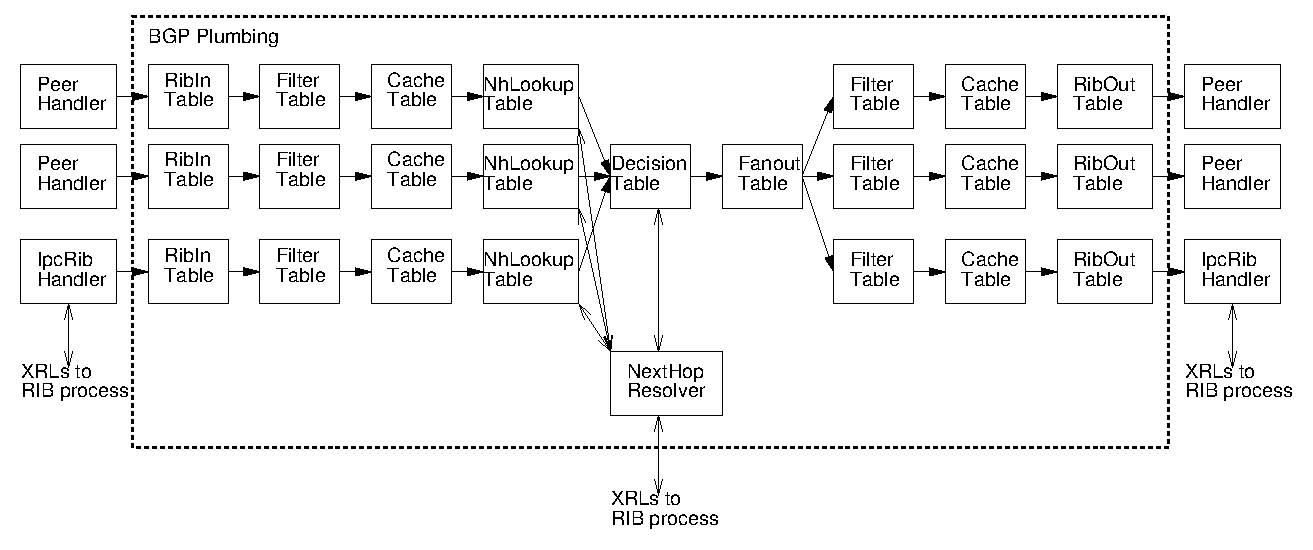
\includegraphics[width=1.0\textwidth]{figs/overview}}
\vspace{.05in}
\caption{\label{overview}Overview of BGP process}
\end{figure}

Route information flows from left to right in this figure.  Typically
an Update or Withdraw message arrives from a BGP peer, is split up
into separate {\tt add\_route} or {\tt delete\_route} commands by the
PeerHandler, and then the update flows through the tables towards the
DecisionTable.  If the route is better than the best alternative, then
it passes through the DecisionTable, and is then fanned out to all the
output branches except the one it arrived un.  The outgoing
PeerHandler then sends the route on to the corresponding BGP peer.

There is one input branch and one corresponding output branch for each
BGP peer, plus one branch that handles routes sent to BGP from the
XORP RIB, and sends BGP routes to the XORP RIB and hence on to the
forwarding engine.  The general structure of the RIB branch is
identical to that of a peer-related branch, but a special version of
the PeerHandler is used.

%%%%%%%%%%%%%%%%%%%%%%%%%%%%%%%%%%%%%%%%%%%%%%%%%%%%%%%%%%%%%%%%%%%%%%%
\section{Major BGP Classes}
In this section we discuss each of the classes from Figure \ref{overview} in
turn, before discussing how each BGP peer is handled.  Most of these
classes are implemented using C++ templates for the address family, so
they are capable of handling IPv4 and IPv6 in an identical manner.
\subsection{PeerHandler Class}
The PeerHandler acts as the interface between the BGP Peer class
(which handles BGP peering connections) and all the RouteTables that
comprise the BGP plumbing.  A single PeerHandler instance receives 
BGP Update messages coming from the BGP peer and constructs new BGP
Update messages to send to that peer.

A BGP Update Message consists of three parts:

\begin{itemize}
  \item A list of withdrawn route subnets (route prefixes).
  \item Path Attribute information for announced routes.
  \item A list of subnets (route prefixes) that are being announced.
	The Path Attribute information applies to all these subnets.
\end{itemize}

The PeerHandler splits an incoming update message up, and constructs a
series of messages (InternalMessage class) to send to the plumbing.

Each of the withdrawn route subnets is passed to the plumbing using a
separate {\tt delete\_route} call.

Each of the announced route subnets is passed to the plumbing using a
separate {\tt add\_route} call, which includes all the Path Attribute
information.

On the output side, the PeerHandler receives a series of {\tt add\_route},
{\tt delete\_route}, or \\
{\tt replace\_route} calls.  Each batch of calls is for
routes that share the same path attribute list.  The PeerHandler then
constructs an Update Message from each batch, and passes it on to the
classes that handle the peering for transmission to the relevant BGP
peer router. 

In some cases the PeerHandler can receive routes from BGP faster than
the connection to the relevant peer can handle them.  The PeerHandler
can communicate this information back upstream to regulate the flow of
changes to a rate that can be accommodated.  The actual queuing then
happens upstream in the FanoutTable.

Because of the way BGP encodes IPv6 routes, the PeerHandler class
handles IPv4 and IPv6 routing information differently.

%%%%%%%%%%%%%%%%%%%%%%%%%%%%%%%%%%%%%%%%%%%
\subsection{RibInTable Class}

The RibInTable class is responsible for receiving routes from the
PeerHandler and storing them.  These are the raw routes, unfiltered
and unmodified except for syntactic correctness, as received and
decoded from the BGP Peering session.

Because BGP does not indicate in an Update message whether a route is
new or merely replaces an existing route, all routes are checked to
see if they are already stored in the RibIn.  If so, the {\tt add\_route} is
propagated downstream as a {\tt replace\_route}, otherwise it is propagated
as an {\tt add\_route}.

The RibIn serves several additional purposes:

\begin{itemize}
  \item It can answer {\tt lookup\_route} requests from downstream.
  \item When a new peer comes up, a route dump is initiated so that the
	new peer learns all the feasible routes that we know.  The RibIn
	can perform this dump as part of a background task, so as to
	allow further updates while the dump is taking place.
  \item When the peer associated with the RibIn goes down, a process to
	delete all the routes learned from this peer is started.  This
	is done by transferring the RibIn's entire routing table to a
	new RouteTable called a DeletionTable that is plumbed in
	directly after the RibIn. The DeletionTable handles the deletion
	of the routes as a background task, leaving the RibIn ready to
	cope immediately if the peer comes back up again.
  \item When the routing information in the XORP RIB changes, the change
	of IGP metric can change which routes should win the decision
	process.
	The RibIn can be told that the routing information associated
	with the indirect nexthop in a BGP route has changed, and it can
	initiate a background task that re-sends all the relevant routes
	downstream as {\tt replace\_route} messages, so that the
	DecisionTable can make its choice again.
\end{itemize}

The RibIn does not do significant sanity checking on its inputs - it
is the responsibility of the receive code in the Peer classes to check
that received update messages are syntactically and semantically
valid.

The current (August 2006) version of XORP stores all routes in the RibIn,
irrespective of whether or not they will fail to pass a downstream
filter.  However, the RibIn has enough information (from the values
returned by the {\tt add\_route}, {\tt delete\_route} and {\tt
replace\_route} calls it makes downstream) to be able to store only
those routes that will not be filtered.

%%%%%%%%%%%%%%%%%%%%%%%%%%%%%%%%%%%%%%%%%%%
\subsection{FilterTable Class}

The FilterTable class has one parent (upstream) RouteTable and one
child (downstream) RouteTable.  It acts as a general purpose
filter-bank, passing, modifying, or dropping routing information that
travels from parent to child.

A FilterTable can hold many filters.  Current filters include:

\begin{itemize}
  \item {\bf SimpleASFilter:}  Drops routes that contain the configured
	AS in their AS Path.
  \item {\bf ASPrependFilter:} Prepends the configured AS number to the
	AS Path of all routes that pass through the filter.
  \item {\bf NexthopRewriteFilter:} Changes the NextHop attribute of all
	routes that pass through the filter to the specified value.
  \item {\bf IBGPLoopFilter:} Drops all routes that we heard through
	IBGP.  This is primarily useful as an outbound filter to an IBGP peer.
  \item {\bf LocalPrefInsertionFilter:} Inserts the configured value as
	the BGP Local Preference attribute in all routes that pass through the
	filter.  Typically used on input from an EBGP peer, before
	route-specific filters.
  \item {\bf LocalPrefRemovalFilter:} Removes the BGP Local Preference
	attribute from all routes that pass through the filter.  Typically
	used on output to an EBGP peer.
  \item {\bf MEDInsertionFilter:} Adds a Multi-exit Descriminator
	attribute based on the routes IGP metric to each route that passes
	through the filter.  Typically used on output to an EBGP peer.  Note
	that the MED to be inserted will have been added to the route by the
	DecisionTable, so MEDInsertionFilter cannot be used as an input-branch
	filter.
  \item {\bf MEDRemovalFilter:} Removes the  Multi-exit Descriminator
	attribute from all routes that pass through the filter.  Typically
	used just before a MEDInsertionFilter to remove the MED received from
	the previous AS.
\end{itemize}

Note that filters are not just for operator configured filtering -
they comprise part of the basic BGP processing mechanism.

Typically a FilterTable will receive an InternalMessage from its
parent containing a subnet route.  All the configured filters will be
applied in order to the route.  One of three things may happen:

\begin{itemize}
  \item The route may be dropped by a filter.
  \item The route may pass through all filters unchanged.
  \item One or more filters may modify the route.  This is done by
	creating a new copy of the route.
\end{itemize}

In the last case, the modified route will have the Changed flag set
before it is propagated downstream.  This flag indicates that no-one
upstream is storing a persistent copy of this route, so the downstream
tables are responsible for either storing the route or freeing the
memory it uses.

Filter implementors should be careful to note that if the route
received as input to a filter is already modified, and their filter
then drops the route or creates a modified copy of the route, then the
old route MUST be freed because no-one else can do so.  If the input
route is not modified, the filter MUST NOT free the route because it
is stored elsewhere.

%%%%%%%%%%%%%%%%%%%%%%%%%%%%%%%%%%%%%%%%%%%
\subsection{CacheTable Class}

The CacheTable class has one parent RouteTable and one child
RouteTable.  Its purpose is to ensure that routes changed by preceding
filter-banks are actually stored somewhere.  Primarily it is an
optimization to prevent the filters from having to be applied every
time {\tt lookup\_route} is called, but it also simplifies memory management
because downstream tables no longer need to be concerned with whether
a route needs to be freed or not. 

The CacheTable takes as input InternalMessages from its parent, and
passes them through downstream to its child.  If the route in the
message does not have the Changed flag set, then the CacheTable is a
no-op.  If the route in the message has the Changed flag set, then the
CacheTable will store the route (or delete it from storage in the case
of {\tt delete\_route}).  Thus all InputMessages sent downstream have the
Changed flag cleared.

A CacheTable in the outgoing branch is flushed (all stored routes
deleted) when the peering corresponding to the relevant plumbing
branch down.  This is because when the peering comes back up, the
outgoing branch should restart with no stored state.  The incoming
branch CacheTable is not explicitly flushed, because the routes will
be removed as the DeletionTable gets round to deleting them.
Prematurely flushing the input branch CacheTables would potentially
result in the DecisionTable seeing inconsistent inputs.

Note that assertion failures in the CacheTable usually indicate that
the code upstream is incorrectly propagating changes (for example
either a delete with no add, two deletes, or two adds).

%%%%%%%%%%%%%%%%%%%%%%%%%%%%%%%%%%%%%%%%%%%
\subsection{NhLookupTable Class}

The BGP decision process implemented in DecisionTable is relatively
complex, and takes into account many possible factors including ``IGP
distance''.  IGP distance is the IGP routing metric for the route to
reach the BGP NextHop (which is often a number of IP hops away in the
case of IBGP).  Also of interest is whether the BGP NextHop is
actually reachable according to the IGP protocols.  Because of the
multi-process architecture of XORP, BGP does not know the IGP distance
or whether the nexthop is reachable.  To find out this information,
BGP must query the RIB, and this is done by the NextHopResolver class
instance.  If DecisionTable had to perform this lookup, it would
become very complex because it would have to handle suspending the
decision process while waiting for results from the RIB.  A
multi-threaded implementation would solve this problem, but would
cause other issues.

To solve these problems we insert an NhLookupTable upstream of the
DecisionTable.  NhLookupTable queues any updates with NextHop
information that the NextHopResolver does not know about, pending the
response from the RIB process.  Thus by the time an update reaches the
DecisionTable, the NextHopResolver already has access to the IGP
information related to the BGP NextHop.

A complication comes with {\tt lookup\_route}:

\begin{itemize}
  \item if the lookup matches an {\tt add\_route} in the NhLookupTable queue,
	the NhLookupTable must return ``lookup unsuccessful''.
  \item if the lookup matches a {\tt replace\_route} entry in the
	NhLookupTable's queue, the old answer must be given.
\end{itemize}

In general, the behaviour should be as if the queued updates had not
yet been received from the relevant peer.  Note that the time for the
RIB to respond should normally be very small compared to the usual
delays for propagating Update messages between peers.

%%%%%%%%%%%%%%%%%%%%%%%%%%%%%%%%%%%%%%%%%%%
\subsection{DecisionTable Class}

The DecisionTable is the core of the BGP process.  It takes route
changes from the input branches, and decides whether those changes are
better or worse than the routes it has already seen.

When DecisionTable receives an {\tt add\_route} from one input branch,
it queries the other peers input branches using {\tt lookup\_route}.

\begin{itemize}
  \item If none of the other branches returns an answer, then the route is a
	new one, and can be passed on downstream so long as the BGP NextHop is
	resolvable.
  \item If one or more of the other branches returns an
	answer, one of these answers will have been the previous winner.  The
	new route is compared against the previous winner - if it is better
	then a {\tt replace\_route} message is propagated downstream.  If it
	is worse, then no further action is taken.
\end{itemize}

When DecisionTable receives a {\tt delete\_route} from one input
branch, it queries the other peers' input branches in the same way:

\begin{itemize}
  \item If none of the other branches returns an answer, the the {\tt
	delete\_route} can be passed on downstream so long as the BGP NextHop
	was previously resolvable.
  \item If one or more of the other branches returns an
	answer, one of these answers will be the new winner.  The routes are
	compared, and a {\tt replace\_route} will be sent downstream.
\end{itemize}

The processing for {\tt replace\_route} is similar to that for {\tt
delete\_route} followed by {\tt add\_route}, except that only a single
replace (or delete in the case where the new nexthop is unreachable
and there are no alternatives) will be sent downstream.

%%%%%%%%%%%%%%%%%%%%%%%%%%%%%%%%%%%%%%%%%%%
\subsection{NextHopResolver Class}

Unlike most of the previous classes, NextHopResolver is not a
RouteTable sub-class.  A BGP implementation has a single NextHopResolver
instance per address family.  The NextHopResolver takes requests to
resolve a BGP NextHop address and attempts to resolve the address to
that of the immediate neighbor router that would be used to forward
packets to the NextHop address.

When it receives an address to resolve, the NextHopResolver first
checks its own routing table.  If the nexthop address can be resolved
there, then the answer can be returned immediately.  Alternatively, if
its own routing table indicates that the address definitely cannot be
resolved, then a negative response can be given immediately.
Otherwise it needs to contact the XORP RIB using XRLs to answer the
question.  

In this way, the NextHopResolver obtains a copy of the relevant subset
of the RIBs database related to the NextHops given by BGP.  The RIB
will also keep track of the subset that it has told BGP about.  If
this information changes in any way BGP will be informed by the RIB,
either directly of the change or that some information is no longer
correct and BGP must query again.

The information held by the NextHopResolver is reference-counted so
that it can be removed when it is no longer relevant.  If the
information contained changes, a notification of the change will be
passed to the DecisionTable, which will propagate the notification
back upstream to the RibIn tables.

%%%%%%%%%%%%%%%%%%%%%%%%%%%%%%%%%%%%%%%%%%%
\subsection{FanoutTable Class}

The principle task of the FanoutTable is to distribute route changes
that passed the DecisionTable, and therefore are real changes not just
possible changes.  FanoutTable passes a change to all the output
branches except the one where the change originated.  In the case of
{\tt add\_route} or {\tt delete\_route}, this is simple but a {\tt
replace\_route} may contain an old route and a new route that
originate from different peers, so it may be propagated as an {\tt
add\_route} to the peer where the old route originated, as a {\tt
delete\_route} to the peer where the new route originated, and as a
{\tt replace\_route} to all the other peers.

The secondary task of the FanoutTable is to serve as a queuing point
for changes when the BGP peers are not capable of keeping up with
updates at the rate we are propagating them.  The advantage of queuing
updates in the FanoutTable as opposed to in the RibOut or PeerHandler
is that only one copy of the change needs to be kept, no matter how
many peers are not keeping up.  This is particularly important in the
case where the peer from which we heard most of our routes goes down,
and a large number of deletions occur in a short period of time.
These deletions need to go to all the remaining peers, and it is
likely that we can generate them faster than TCP can transfer them to
the peer.

Thus there is a single update queue in the FanoutTable, and a separate
pointer into this queue is maintained for each outgoing branch (and
hence each peer).  If a output branch indicates it is busy, the
FanoutTable will stop propagating changes to it, and instead queue the
changes.  Only when a change has been propagated to all the intended
peers will it be removed from the queue.  

%%%%%%%%%%%%%%%%%%%%%%%%%%%%%%%%%%%%%%%%%%%
\subsection{RibOutTable Class}

The purpose of the RibOutTable is to communicate changes to the
outgoing PeerHandler and hence on to the relevant BGP peer.  The
RibOutTable class accumulates changes (add, delete or replace) in a
queue, and waits for a flush request.  The reason for the queue is
that the incoming PeerHandler split up a single incoming Update message
into many changes, each with the same Path Attributes.  On output, we
want to accumulate these changes again, so that we can send them on to
our peers in a single Update message.  Thus, after the incoming
PeerHandler has sent the last change to the RibIn, it sends a flush
message through.  When this reaches the RibOut, it is the signal to
take all the changes that have been queued, and build one or more
Update messages from them.  Of course the nature of the decision
process and filters mean that changes that arrived together do not
always result in outgoing changes that share the same Path
Attributes.  Thus multiple passes over the RibOut queue are required,
each accumulating changes that share the same Path Attributes so that
they can be sent on in the same Update message.

In principle, the RibOut could also store pointers to the routing
information that was passed on to the peer so that Route Refresh
(RFC 2918) could be handled efficiently.  In our current implementation
we do not do this - the RibOut maintains no record of the routes
passed to the peer.

%%%%%%%%%%%%%%%%%%%%%%%%%%%%%%%%%%%%%%%%%%%
\subsection{RibIpcHandler Class}

The RibIpcHandler class is a subclass of PeerHandler, with basically
the same interface as far as communication with the RibIn and RibOut
are concerned. However, instead of communicating with BGP peers, the
RibIpcHandler communicates routes to and from the XORP RIB.  Routes
are received from the RIB if the RIB has been configured to
redistribute routes to BGP.  In addition, all routes we pass to other
peers are also communicated to the XORP RIB, and hence on to the
forwarding engine, so that we can forward packets based on the routing
information.

%%%%%%%%%%%%%%%%%%%%%%%%%%%%%%%%%%%%%%%%%%%%%%%%%%%%%%%%%%%%%%%%%%%%%%%
\section{Background Tasks}

The XORP BGP implementation, like all XORP processes, is
single-threaded.  However, certain simple events can cause BGP to
perform a great deal of work.  For example:

\begin{itemize}
  \item When a peering goes down, all the routes in the RibIn associated
	with that peer must be deleted, which either results in Withdraws
	being sent to all remaining peers, or Updates being sent to indicate
	an alternative path is now the winner.  As there can be many thousands
	of routes in a RibIn, this process can take some time.
  \item When a new peering comes up, all the winning routes must be sent
	to that peer.  This can also take some time.
  \item When the IGP information related to a BGP nexthop changes, all
	the routes that specify this nexthop must be re-evaluated to see if
	the change affects the choice of route.  In BGP it is fairly common
	for a very large number of routes to share the same BGP nexthop, so
	this re-evaluation can take some time.
\end{itemize}

The XORP BGP process cannot simply process such events to completion -
in particular it must keep processing XRL requests from other
processes or the IPC mechanism may declare a failure.  In any event,
it is important that a single slow peer cannot cause route forwarding
between other peers to stall.  Thus we process the events above as
``background tasks''.  

In a multithreaded architecture, such tasks might be separate threads,
but the locking issues soon become very complex.  In our single
threaded architecture, there are no complex locking issues, but the
background nature of such tasks needs to be explicitly coded.  We do
this by dividing the background task into small enough segments.  At
completion of such a segment we schedule a zero-second timer to
schedule execution of the next segment, and drop back to the main
event loop.  Execution will then be restarted after pending network
events and expired timers have been processed by the main event loop.
Care must of course be taken to ensure that when execution returns,
the processing of events or other background tasks has not rendered
incorrect the state the background task needed to restart.  However,
as the processing of each background task segment is naturally atomic
in a single-threaded architecture, there are fewer possibilities for
bad interactions.  Even so, the state stored by these background tasks
to enable their correct restart involves some rather complex
algorithms.

%%%%%%%%%%%%%%%%%%%%%%%%%%%%%%%%%%%%%%%%%%%
\subsection{DeletionTable Class}

When a peering goes down, the routing table stored in the RibIn is
moved to a DeletionTable that is plumbed in directly after the RibIn,
as shown in figure \ref{del_table}.

\begin{figure}[htb]
\centerline{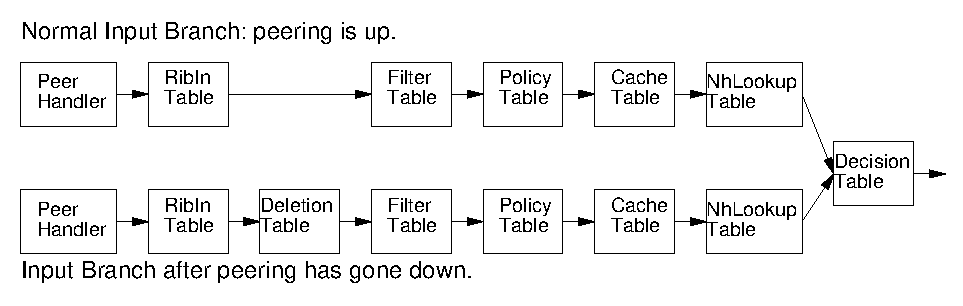
\includegraphics[width=0.7\textwidth]{figs/del_table}}
\vspace{.05in}
\caption{\label{del_table}Dynamic insertion of Deletion Table on
Peering Failure}
\end{figure}

The task of the deletion table is to delete all the routes that were
previously stored in the RibIn, but to do so as a background task
allowing the BGP process to continue to handle new events.

Deletion is scheduled in series of phases.  In a single phase, all the
routes that share a single set of Path Attributes are deleted.  In
this way, if there are alternative routes in a different RibIn that
also share a path attribute list (a fairly common occurrence), then the
chance of preferred route may be batched in such a way that it might be
possible to use a single update message might convey the change to
each neighbor.  At the end of a phase, the DeletionTable schedules
execution of the next deletion phase using a zero-second timer.  This
allows all pending timer or network events to be handled before
deletion resumes.

The DeletionTable must respond to {\tt lookup\_route} requests from
downstream just as a RibIn table would - even though the deletion
table knows the routes it holds will be deleted, it must respond as if
they had not yet been deleted until it has had a chance to send the
relevant {\tt delete\_route} message downstream.  In this way, the
DeletionTable provides a consistent view to the downstream tables - if
they earlier performed a {\tt lookup\_route} and got a specific answer,
then they will still get the same answer unless they have received a
{\tt delete\_route} or {\tt replace\_route} informing them of a
change.

When the last route is deleted from the DeletionTable, the table
unplumbs itself from the BGP plumbing, and deletes itself.

A small complication is added by the possibility that the peering
might come back up before the DeletionTable has finished deleting all
the old routes.  Thus if the DeletionTable receives an {\tt
add\_route} from upstream for a route that in present in the
DeletionTable, then this route would be passed on downstream as a {\tt
replace\_route}, and the route would then immediately be removed from
the DeletionTable.  {\tt add\_route}, {\tt replace\_route} and {\tt
delete\_route} for routes not present in the DeletionTable are simply
passed from parent to child without modification.

Should the peering come up and go down again before all the routes in
the first DeletionTable have been deleted, a second deletion table
would be inserted before the first one.  By virtue of the normal
functioning of the DeletionTable, if there are two such cascaded
DeletionTables, then they will not hold the same route, so this does
not add any additional complication.

%%%%%%%%%%%%%%%%%%%%%%%%%%%%%%%%%%%%%%%%%%%
\subsection{DumpTable Class}

When a peering comes up, all the currently winning routes from the
other peers must be sent to the new peer.  This process is managed by
an instance of the DumpTable class, which is inserted between the
fanout table and the first table on the output branch to the peer that
came up (see Figure \ref{dump_table}).

\begin{figure}[htb]
\centerline{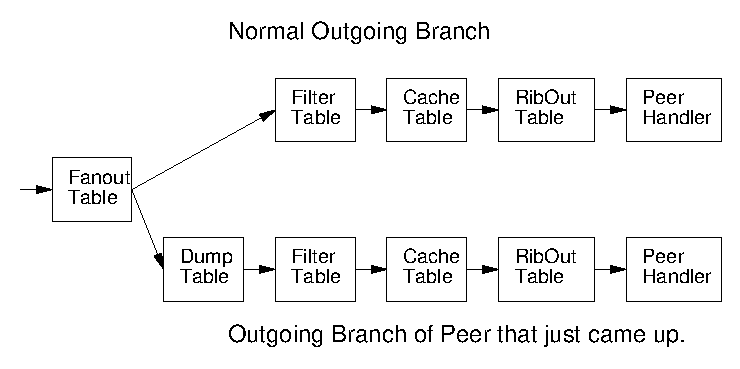
\includegraphics[width=0.6\textwidth]{figs/dump_table}}
\vspace{.05in}
\caption{\label{dump_table}Dynamic insertion of DumpTable on
a peering coming up.}
\end{figure}

A DumpTable is perhaps the most complex part of the BGP machinery.
While the dump is taking place, it must cope with:

\begin{itemize}
  \item New routing information being propagated.
  \item Other peers going down and coming back, possibly repeatedly.
\end{itemize}

It must do this without propagating inconsistent information downstream,
such as a {\tt replace\_route} or a {\tt delete\_route} without
sending an {\tt add\_route} first.  It must ensure that all the routes
what passed decision are dumped to the new peer. And it must cope when
the routes just before and just after the most recent route it dumped
are deleted, without losing track of where it is in the dump process.

The process is complex enough to merit description here in detail.

Each DumpTable contains a DumpIterator instance which holds all the
state related to the current state of that particular route dump.  The
DumpIterator contains the following state:

\begin{itemize}
  \item A list of the remaining peers to dump, initialized at the start
	of the dump.  Peers are removed from this list when the dump of the
	routes received from that peer is complete, or when the peer does down
	during the dump.  Peers are never added to this list during the dump.
  \item A list of the peers that went down before we'd finished dumping
	them.  Along with each peer is stored enough state to know how far
	we'd got though the route dump from that peer before it went down.
  \item The current peer whose routes are being dumped.
  \item A trie iterator pointing to the next RibIn trie entry to be dumped
	on the current peer (we call this the Route Iterator)
  \item The last subnet dumped from the current peer.
  \item A flag that indicates whether the Route Iterator is currently
	valid.
  \item The last GenID seen.  The GenID of the RibIn is incremented each
	time the peering comes up.
\end{itemize}

At startup the DumpTable initialized the list of remaining peers in
the DumpIterator to be the set of peers that are currently up.  Then
it iterates through this list dumping all the routes from each RibIn
in turn.

The DumpTable calls {\tt dump\_next\_route} on its parent table, passing the
DumpIterator as a parameter.  The {\tt dump\_next\_route} request is relayed
upstream to the DecisionTable.  DecisionTable relays the request to
the input branch of the first peer listed in the list of remaining
peers, and from there it is relayed back to the relevant RibIn.

To allow routes in the RibIn to be deleted during the route dump
without the Route Iterator becoming invalid, we use a special trie and
trie iterator in RibIn, where the route in the trie will not actually
be deleted until no trie iterator is pointing at it.  This is
implemented using reference counts in the Trie nodes themselves.

{\tt dump\_next\_route} in the RibIn checks the Route Iterator to see
if it points to the end of the Trie.  If the previous call to {\tt
dump\_next\_route} had left the Route Iterator pointing to a node that has
subsequently been deleted, this comparison transparently causes the
Route Iterator to move on to the next non-deleted node, or to the end
of the Trie if there are no subsequent deleted nodes.  This updating
of the Route Iterator is transparent to the user of the iterator.

The route pointed to by the Route Iterator is then propated downstream
from the RibIn to the DumpTable as a {\tt route\_dump} call.  The
DumpTable turns this into an {\tt add\_route} call which it propagates
downstream to the new peer.

At the end of {\tt dump\_next\_route}, the RibIn increments the
RouteIterator ready for next time.  

DumpTable then schedules the next call to {\tt dump\_next\_route} using a
zero-second timer to allow other pending events to be processed.

On returning from the timer, the DumpTable checks to see if any route
changes have been queued upstream in the FanoutTable due to output
flow control.  If so, it processes all these route changes before
dumping the next route.  This is necessary, or the DumpTable will not
be able to tell which changes it needs to propagate downstream because
we've already passed their location in the dump process, and which are
unnecessary because we will get round to dumping them eventually.

In general, a route
change needs to be propagated downstream if:

\begin{itemize}
  \item It comes from a peer that is not in our remaining peers list.
  \item It comes from the peer currently being dumped, but its route is
	before the location of the route in the DumpIterator.
  \item It comes from a peer that went down, and its subnet is before the
	subnet we had reached while dumping that peer's RibIn when the peer
	went down.
  \item It comes from a peer that went down, and the RibIn GenID later
	than that peers GenID was when it went down.  This would happen
	because the peering has since come back up, and is now injecting new
	routes.
\end{itemize}

When all the routes in the RibIn of a particular peer have been
dumped, that peer is removed from the remaining peers list in the
DumpIterator, and the next {\tt dump\_next\_route} will be sent to the RibIn
of the next peer in the list.

When there are no peers in the remaining peers list, the dump is
complete.  The DumpTable then unplumbs itself from the plumbing, and
deletes itself.

Note that at any time there may be multiple DumpTables in operation,
each dumping to a different peer.  All the dump state is held in the
DumpIterators, so this does not cause any problem.

%%%%%%%%%%%%%%%%%%%%%%%%%%%%%%%%%%%%%%%%%%%%%%%%%%%%%%%%%%%%%%%%%%%%%%%
%     APPENDIX
%%%%%%%%%%%%%%%%%%%%%%%%%%%%%%%%%%%%%%%%%%%%%%%%%%%%%%%%%%%%%%%%%%%%%%%
\appendix
\section{Modification History}

\begin{itemize}
  \item December 11, 2002: Version 0.1 completed.
  \item March 10, 2003: Updated to match XORP version 0.2 release code;
	cleanup.
  \item June 9, 2003: Updated the version to 0.3, and the date.
  \item August 28, 2003: Updated the version to 0.4, and the date.
  \item November 6, 2003: Updated the version to 0.5, and the date.
  \item July 8, 2004: Updated the version to 1.0, and the date.
  \item April 13, 2005: Updated the version to 1.1, and the date.
  \item March 8, 2006: Updated the version to 1.2, and the date.
\end{itemize}


%%%%%%%%%%%%%%%%%%%%%%%%%%%%%%%%%%%%%%%%%%%%%%%%%%%%%%%%%%%%%%%%%%%%%%%
%     BIBLIOGRAPHY
%%%%%%%%%%%%%%%%%%%%%%%%%%%%%%%%%%%%%%%%%%%%%%%%%%%%%%%%%%%%%%%%%%%%%%%
\bibliography{../tex/xorp}
\bibliographystyle{plain}

%%%%%%%%%%%%%%%%%%%%%%%%%%%%%%%%%%%%%%%%%%%%%%%%%%%%%%%%%%%%%%%%%%%%%%%
\end{document}

%
% $XORP: xorp/docs/user_manual/policy.tex,v 1.11 2006/04/13 06:36:58 pavlin Exp $
%

\chapter{\label{policy}Policy}
Policy controls which routes to accept and which routes should be advertised.
Moreover, it provides a mechanism for modifying route attributes and enables
{\em route redistribution} which allows routes learnt by a protocol to be
advertised by a {\em different} protocol.


\section{Terminology and Concepts}
A crucial aspect to understand is the difference between {\em import} and {\em
export} policies.
%
\begin{description}
\item[import] filters act upon routes as soon as they are received from a
routing protocol.  Before a protocol even makes a decision on the route, import
filter processing will already have taken place.  Note that import filters may
therefore affect the decision process (e.g. by changing the metric).
%
\item[export] filters act upon routes just before they are advertised by a
routing protocol.  Only routes which have won the decision process (i.e. the
ones used in the forwarding plane) will be considered by export filters.
\end{description}

Normally policies will operate within a single routing protocol, for example  a
policy which sets the MED on all BGP routes (only BGP is involved).  If a policy
involves two different protocols, then {\em route redistribution} will occur
``implicitly''.

\section{Policy Statement}
A {\em policy statement} is the user definition for a policy.  Internally, it
contains a list of {\em terms}.  A term is the most atomic unit of execution of
a policy.  Each single term, if executed, will cause actions to be taken on a
route.  A policy statement should define a logical operation to be run on
routes and this operation may involve multiple terms, which define simpler and
smaller execution steps.

The overall structure of a policy statement looks as follows:

\noindent\framebox[\textwidth][l]{\scriptsize
\begin{minipage}{6in}
\begin{alltt}
\begin{tabbing}
xx\=xx\=xx\=xx\=xx\=\kill
policy \{\\
\>policy-statement {\em name} \{\\
\>\>term {\em name} \{\\
\>\>\} \\
\>\>\ldots \\
\>\>term {\em name} \{\\
\>\>\} \\
\>\} \\
\}
\end{tabbing} 
\end{alltt}
\end{minipage}
}

Each term of a policy is executed in order.  It is not required that {\em all}
terms run---it is possible for a term to cause the policy to accept or
reject the route terminating the overall execution.

Once a policy is specified, it must be {\em bound} (applied) to a protocol.
This is achieved via the {\tt import} or {\tt export} statement depending on
the type of policy, within a protocol block.  For example:

\noindent\framebox[\textwidth][l]{\scriptsize
\begin{minipage}{6in}
\begin{alltt}
\begin{tabbing}
xx\=xx\=xx\=xx\=xx\=\kill
protocol \{\\
\>bgp \{\\
\>\>export: "policy1,policy2,\ldots"\\
\>\>import: "drop\_bad"\\
\>\} \\
\}
\end{tabbing} 
\end{alltt}
\end{minipage}
}

It is possible to have multiple policy statements per protocol such as in the
{\tt export} example above.  The policies, like terms, will be executed in
order.  Again, it is possible that not all policies are run---maybe the first
one will cause an accept or reject.

\subsection{Term}
A term is the heart of the policy execution.  It specifies how to match routes
as they enter the system, as they are about to leave and ultimately what
actions to perform on them.  The structure of a term is as follows:

\noindent\framebox[\textwidth][l]{\scriptsize
\begin{minipage}{6in}
\begin{alltt}
\begin{tabbing}
xx\=xx\=xx\=xx\=xx\=\kill
term {\em name} \{\\
\>from \{\\
\>\>\ldots\\
\>\} \\
\>to \{\\
\>\>\ldots\\
\>\} \\
\>then \{\\
\>\>\ldots\\
\>\} \\
\}
\end{tabbing} 
\end{alltt}
\end{minipage}
}

It is possible to omit the {\tt from}, {\tt to} and {\tt then} block.  If so,
{\tt from} and {\tt to} will match {\em all} routes traversing the filter.  An
empty {\tt then} block will run the {\em default action}.  The default action is
to execute the next term / policy in the list or accept the route if the last
term is being run.

In general, the {\tt from} and {\tt to} block will specify the {\em match
conditions} on a route and the {\tt then} block the actions to be performed on
the route in case of a match.

\subsubsection{Match Conditions}
The overall structure of a match condition is: {\em variable}, {\em operator},
{\em argument}.  A variable is a route attribute such as metric, prefix,
next-hop and so on.  The operator will specify {\em how} this variable is
matched.  For example {\tt $<$} may perform a less-than match whereas {\tt $>$}
may perform a greater-than operation.  The argument will be the value against
which the variable is matched.  The overall result is a {\em logical and} with
the result of each statement. An example would be as follows:

\noindent\framebox[\textwidth][l]{\scriptsize
\begin{minipage}{6in}
\begin{alltt}
\begin{tabbing}
xx\=xx\=xx\=xx\=xx\=\kill
from \{\\
\>protocol: "static"\\
\>metric < 5\\
\} \\
to \{\\
\>neighbor: 10.0.0.1\\
\} \\
then \{\\
\>\ldots\\
\} \\
\end{tabbing} 
\end{alltt}
\end{minipage}
}

In this example {\tt metric} is a variable, {\tt $<$} an operator and {\tt 5}
the argument.  This will match all static routes with a metric less than 5 being
advertised to the neighbor 10.0.0.1.  Note that the {\tt :} operator is an alias
for {\tt $==$} when matching (in {\tt from} and {\tt to} blocks) which simply
means equality.

\subsubsection{Actions}
All actions are performed sequentially and have a similar syntax to match
conditions. The main difference with respect to match conditions is that the
operator will normally be assignment and that special {\em commands} exist.
These commands are {\tt accept} and {\tt reject}.  If a route is accepted, no
further terms will be executed and the route will be propagated downstream.  If
a route is rejected, once again no further terms will run, and the route will {\em
not} be propagated downstream---it will be suppressed and dropped.  Depending on
whether it is an export or import filter, reject will have different semantics.
On export it will not be advertised and on import it will never be used at all.  

Here is an example of the syntax used when specifying actions:

\noindent\framebox[\textwidth][l]{\scriptsize
\begin{minipage}{6in}
\begin{alltt}
\begin{tabbing}
xx\=xx\=xx\=xx\=xx\=\kill
from \{\\
\>\ldots\\
\} \\
to \{\\
\>\ldots\\
\} \\
then \{\\
\>metric: 5\\
\>accept\\
\} \\
\end{tabbing} 
\end{alltt}
\end{minipage}
}

This term will cause the metric to be set to 5 and no further terms will be
executed, because of the {\tt accept}. Note that in the case of {\tt then}
blocks, the {\tt :} operator is an alias for {\tt =} which means assignment.

If neither {\tt accept} nor {\tt reject} are specified, the default action will
occur.  The default action will execute the next term or accept the route if the
last term has been reached.

Note that if the {\tt then} block contains an {\tt accept} or {\tt reject}
action, all other actions within the {\tt then} block will be executed
regardless whether in the configuration they are placed before or after
the {\tt accept} or {\tt reject} statements.

\section{Sets}
Many times it is useful to match against a set of values.  For example it is
more practical to reference a set of prefixes to match against, which may also
be used in different policies rather than enumerating the prefixes one by one in
each policy.  This is achieved via sets which contain un-ordered items and no
duplicates.  Sets are declared as follows:

\noindent\framebox[\textwidth][l]{\scriptsize
\begin{minipage}{6in}
\begin{alltt}
\begin{tabbing}
xx\=xx\=xx\=xx\=xx\=\kill
policy \{\\
\>network4-list {\em name} \{ \\
\>\>elements: "10.0.0.0/8,192.168.0.0/16,\ldots"\\
\>\}\\
\>network6-list {\em name} \{ \\
\>\>elements: "2001:0910::/32,2001:dead::/32,\ldots"\\
\>\}\\
\} \\
\end{tabbing} 
\end{alltt}
\end{minipage}
}

Two sets cannot have the same name---else there is no way to reference them
within policies.  Sets of different types are created in different ways.  For
example, a set of IPv4 prefixes is created via the {\tt network4-list} directive
whereas IPv6 prefixes would be created using {\tt network6-list}.  To reference
a set in a policy, simply use its name as a text string.  For example:

\noindent\framebox[\textwidth][l]{\scriptsize
\begin{minipage}{6in}
\begin{alltt}
\begin{tabbing}
xx\=xx\=xx\=xx\=xx\=\kill
policy \{\\
\>network4-list private \{ \\
\>\>elements: "10.0.0.0/8,192.168.0.0/16"\\
\>\}\\
\>policy-statement drop-private \{ \\
\>\>term a \{\\
\>\>\>from \{\\
\>\>\>\>network4-list: "private"\\
\>\>\>\}\\
\>\>\>action \{\\
\>\>\>\>reject\\
\>\>\>\}\\
\>\>\}\\
\>\} \\
\} \\
\end{tabbing} 
\end{alltt}
\end{minipage}
}

This policy will match when the route is 10.0.0.0/8 or 192.168.0.0/16.  In this
case the match needs to satisfy only one element of the set.  This is not always
the case.  If a route attribute which actually {\em is} a set (such as BGP
communities) was matched against a set the user specifies, depending on the
operator, different semantics would apply.  For example an operator may check
that the sets are equal, or that one has to be the subset of the other and so
on.  Obviously in this case each route has a single prefix so the only
reasonable match would be to check whether that prefix is in the set or not.

Note that it is pure ``coincidence'' that the directive to match a list of
prefixes {\tt network4-list} is the same as the one used to declare the set.  It
is not a requirement.

\section{Ranges}
Certain variables can be matched against linear ranges of their corresponding type.
The policy engine supports matching against ranges of unsigned integers and IPv4 / IPv6 addresses.
Ranges are expressed by specifiying their lower and upper inclusive boundaries separated by two dots, for example:

\noindent\framebox[\textwidth][l]{\scriptsize
\begin{minipage}{6in}
\begin{alltt}
\begin{tabbing}
xx\=xx\=xx\=xx\=xx\=\kill
from \{\\
\>nexthop4: 10.0.0.11..10.0.0.15\\
\>neighbor: 10.0.0.0..10.0.0.255\\
\>med: 100..200\\
\} \\
\end{tabbing} 
\end{alltt}
\end{minipage}
}

An abbreviated form of specifying a range containing a single value is allowed, in which case both the lower and upper boundary are considered to be equal.  Hence, the following two expressions are equivalent:

\noindent\framebox[\textwidth][l]{\scriptsize
\begin{minipage}{6in}
\begin{alltt}
\begin{tabbing}
xx\=xx\=xx\=xx\=xx\=\kill
from \{\\
\>neighbor: 10.1.2.3\\
\>med: 100\\
\} \\
from \{\\
\>neighbor: 10.1.2.3..10.1.2.3\\
\>med: 100..100\\
\} \\
\end{tabbing} 
\end{alltt}
\end{minipage}
}


\section{Tracing}
It is often useful to trace routes going through filters in order to debug
policies.  Another utility of this would be to log specific routes or simply to
monitor routes flowing throughout XORP.  This functionality is achieved via policy
tracing.

In order to trace a particular term simply assign an integer to the {\tt trace}
variable in the {\tt then} block.  The higher the integer, the more verbose the
log message is.  Here is an example:

\noindent\framebox[\textwidth][l]{\scriptsize
\begin{minipage}{6in}
\begin{alltt}
\begin{tabbing}
xx\=xx\=xx\=xx\=xx\=\kill
from \{\\
\>neighbor: 10.0.0.1\\
\} \\
then \{\\
\>trace: 3\\
\}\\
\end{tabbing} 
\end{alltt}
\end{minipage}
}

Assuming this is a BGP import policy, this term would cause all routes learnt
from the BGP peer 10.0.0.1 to be logged verbosely.  Currently there is no useful
meaning associated with the integral verbosity level although 1 normally
indicates a single line of log whereas 3 is the most noisy.

Note that only terms which match may be traced---else the {\tt then} block which
sets up the trace will never be run!  However, it is trivial to put a term which
will match everything (empty {\tt from} and {\tt to} block) which simply enables
tracing.  This may be necessary if {\em all} routes need to be monitored.

\section{Route Redistribution}
Route redistribution is a mechanism for advertising routes learnt via a
different protocol.  An example would be to advertise some static routes using
BGP.  Another possibility is advertising BGP routes using OSPF and so on.  The
key is that the {\tt from} block of a term will be matched in the protocol which
{\em received} the route whereas the {\tt to} block will be matched in the
protocol which is {\em advertising} the route (doing the redistribution).
Route redistribution will always be an export policy---the protocol exporting
(advertising) is the one redistributing.  All actions (such as changing the
metric) will occur in the protocol doing the redistribution.  

Here is an example:

\noindent\framebox[\textwidth][l]{\scriptsize
\begin{minipage}{6in}
\begin{alltt}
\begin{tabbing}
xx\=xx\=xx\=xx\=xx\=\kill
policy \{\\
\>policy-statement "static-to-bgp" \{\\
\>\>term a \{\\
\>\>\>from \{\\
\>\>\>\>protocol: "static"\\
\>\>\>\>metric: 2\\
\>\>\>\}\\
\>\>\>to \{\\
\>\>\>\>neighbor: 10.0.0.1\\
\>\>\>\}\\
\>\>\>then \{\\
\>\>\>\>med: 13\\
\>\>\>\>accept\\
\>\>\>\}\\
\>\>\}\\
\>\} \\
\} \\
\\
protocols \{\\
\>bgp \{\\
\>\>export: "static-to-bgp"\\
\>\}\\
\}\\
\end{tabbing} 
\end{alltt}
\end{minipage}
}

The policy is applied to BGP as it is doing the redistribution.  It is an export
policy because it is advertising.  Since the {\tt from} block contains a
protocol which is not BGP, route redistribution will occur.  In this case, all
static routes with metric 2 will be passed to BGP.  Furthermore, as these routes
are advertised to the BGP peer 10.0.0.1, the MED will be set to 13.

Note that this policy will cause all static routes with metric of 2 to be
advertised to {\em all} BGP peers---not only 10.0.0.1.  This policy does two
things: it sets up the route redistribution, and further more changes the MED 
for a specific peer on those routes.  Other peers will receive the static routes
with the default MED value.  

In order to prevent other peers receiving static routes, another policy should
be appended specifying that all static routes with metric of 2 should be
rejected.  Since this policy is added after the one in the example (in the
{\tt export} statement of BGP) the BGP peer 10.0.0.1 {\em will} receive the
advertisement as no further terms / policies will be executed after the {\tt
accept} of the first policy (which matches).

\section{Common Directives for all Protocols}
All protocols have a common set of route attributes which may be matched,
modified and actions which should take place on a route.  These may be found in
the template file {\tt policy.tp}. 

\subsection{Match Conditions}
Table~\ref{policy_common_match_from} summarizes the match conditions
in a {\tt from} block for all protocols.
\begin{table}[h]
\centering
\begin{tabular}{|l|c|c|p{7.5cm}|}
\hline
Variable & Operator & Argument type & Semantics \\
\hline\hline
{\tt protocol} & {\tt :} & txt & Matches the protocol via which the route was
learnt.  Only valid for export policies.  Used in route redistribution. \\
\hline
{\tt network4} & {\tt :} & ipv4net & Matches the prefix of an IPv4 route. \\
{\tt network6} & {\tt :} & ipv6net & Matches the prefix of an IPv6 route. \\
\hline
{\tt network4-list} & {\tt :} & network4-list & Matches if the IPv4 set contains
the route.\\
{\tt network6-list} & {\tt :} & network6-list & Matches if the IPv6 set contains
the route.\\
\hline
{\tt prefix4-length} & {\tt :} & u32range & Matches if the IPv4 route has a
prefix length within the specified range. \\
{\tt prefix6-length} & {\tt :} & u32range & Matches if the IPv6 route has a
prefix length within the specified range. \\
\hline
\end{tabular}
\caption{\label{policy_common_match_from}Common match conditions in the {\tt from}
block for all protocols}
\end{table}

The match conditions for the {\tt to} block are identical in syntax and
semantics as the {\tt from} block except for one case.  It is illegal to specify
the protocol in the {\tt to} block.  The reason for this is that when a policy
is bound to a protocol via the {\tt export} or {\tt import} statement, that
protocol automatically becomes the one referenced in the {\tt to} block.  When a
BGP export policy is created, the {\tt to} must be BGP by definition as {\em it}
is doing the advertisement.

\subsection{Actions}
Common actions to all protocols are summarized in
table~\ref{policy_common_action}.

\begin{table}[h]
\centering
\begin{tabular}{|l|c|c|p{9cm}|}
\hline
Variable & Operator & Argument type & Semantics \\
\hline\hline
{\tt accept} & none & none & Propagate this route downstream and stop executing
all policies associated to this route.\\
{\tt reject} & none & none & Do not propagate this route downstream and stop executing
all policies associated to this route.\\
\hline
{\tt trace} & {\tt :} & u32 & Enable tracing at a specific verbosity level.
Currently 1 means a single line of logging and 3 is the most verbose level. \\
\hline
\end{tabular}
\caption{\label{policy_common_action}Common actions for all protocols}
\end{table}

\section{BGP}
BGP supports policy and route redistribution.  It can be used both as a source
for redistribution (BGP-to-something) and as a target (something-to-BGP).  The
following sections summarize which aspects of BGP routes may be matched and what
actions may be taken. These are also specified in the {\tt bgp.tp} template file.

The BGP policy engine currently has an interesting feature / bug.  An export
filter is placed on the RIB branch too.  Thus, if an export policy rejects all
routes, the RIB will never receive these routes and no routes will go into the
forwarding plane.  To avoid this, match {\tt neighbor: 0.0.0.0} in the {\tt to}
block and {\tt accept}.  The next term could match all and reject.  This
``feature'' is actually useful if you want a BGP peering but do not wish to
change the routing table.

\subsection{Match Conditions}
Table~\ref{policy_bgp_match} summarizes the match conditions specific to BGP.
\begin{table}[h]
\centering
\begin{tabular}{|l|c|c|p{7cm}|}
\hline
Variable & Operator & Argument type & Semantics \\
\hline\hline
{\tt nexthop4} & {\tt :} & ipv4range & Matches if the IPv4 next-hop of the route
lies within the specified range.\\
{\tt nexhtop6} & {\tt :} & ipv6range & Matches if the IPv6 next-hop of the route
lies within the specified range. \\
\hline
{\tt as-path} & {\tt :} & txt & Matches an AS-Path with a regular expression. \\
{\tt as-path-list} & {\tt :} & as-path-list & If the set contains a regular
expression which matches an AS-Path, then the term matches. \\
\hline
{\tt community} & {\tt :} & txt & Matches against the specified community. \\
{\tt community-list} & {\tt :} & community-list & If the set contains a
community which matches, then the term matches. \\
\hline
{\tt neighbor} & {\tt :} & ipv4range & In a {\tt from} block it matches whether
the route was learnt from a BGP peer in the specified range.  In a {\tt to}
block it matches whether the route is about to be advertised to a BGP peer in
the specified range. \\
\hline
{\tt origin} & {\tt :} & u32 & Matches the origin attribute of the route. 0
stands for IGP, 1 for EGP and 2 for INCOMPLETE.  \\
\hline
{\tt med} & {\tt :} & u32range & Matches the MED of the route. \\
\hline
{\tt localpref} & {\tt :} & u32range & Matches the local preference of the route. \\
\hline
{\tt was-aggregated} & {\tt :} & bool & True if this route contributed to
origination of an aggregate route. \\
\hline
\end{tabular}
\caption{\label{policy_bgp_match}BGP specific match conditions.}
\end{table}

\subsection{Actions}
Table~\ref{policy_bgp_action} summarizes the actions specific to BGP.
\begin{table}[h]
\centering
\begin{tabular}{|l|c|c|p{7cm}|}
\hline
Variable & Operator & Argument type & Semantics \\
\hline\hline
{\tt nexthop4} & {\tt :} & ipv4 & Replaces the IPv4 nexthop. \\
{\tt nexhtop6} & {\tt :} & ipv6 & Replaces the IPv6 nexthop. \\
\hline
{\tt as-path-prepend} & {\tt :} & txt & Prepends the specified AS-Path to the
one on the route. \\
{\tt as-path-expand} & {\tt :} & u32 & Prepends the last AS in the path the
specified number of times. \\
\hline
{\tt community} & {\tt :} & txt &  Sets the community attribute.\\
{\tt community-add} & {\tt :} & txt & Adds the specified community. \\
\hline
{\tt community-del} & {\tt :} & txt & Deletes the specified community. \\
\hline
{\tt origin} & {\tt :} & u32 & Sets the origin. \\
\hline
{\tt med} & {\tt :} & u32 & Sets the MED. \\
\hline
{\tt med-remove} & {\tt :} & bool & Remove MED if present. \\
\hline
{\tt localpref} & {\tt :} & u32 & Sets the localpref. \\
\hline
{\tt aggregate-prefix-len} & {\tt :} & u32 & Originate an aggregate route with
this prefix length. \\
\hline
{\tt aggregate-brief-mode} & {\tt :} & bool & If true omit AS SET generation
in aggregate route. \\
\hline
\end{tabular}
\caption{\label{policy_bgp_action}BGP specific actions.}
\end{table}

\section{Static Routes}
Static routes support policy and may be used as a source for route
redistribution.  The only extra attribute which may be matched on a static route
is {\tt metric} which takes an integer as an argument.  It matches the metric of
the route.  The {\tt static\_routes.tp} template file specifies the route
attributes specific to static routes.

\section{RIP}
RIP supports policy and may be used as a source and target for route
redistribution.

\section{OSPF}
OSPF supports policy and route redistribution.  It can be used both as
a source for redistribution (OSPF-to-something) and as a target
(something-to-OSPF). The following sections summarize which aspects of
OSPF routes may be matched and what actions may be taken. These are
also specified in the {\tt ospfv2.tp} template file.

\subsection{Match Conditions}
Table~\ref{policy_ospf_match} summarizes the match conditions specific to OSPF.
\begin{table}[h]
\centering
\begin{tabular}{|l|c|c|p{7cm}|}
\hline
Variable & Operator & Argument type & Semantics \\
\hline\hline
{\tt nexthop4} & {\tt :} & ipv4range & Matches if the IPv4 next-hop of the route
lies within the specified range.\\

\hline
{\tt metric} & {\tt :} & u32 & Matches metric \\
\hline

\hline
{\tt ebit} & {\tt :} & bool & Matches ebit true for type1 false for type2 \\
\hline

\hline
{\tt tag} & {\tt :} & u32range & Matches tag field in AS-external-LSA \\
\hline

\end{tabular}
\caption{\label{policy_ospf_match}OSPF specific match conditions.}
\end{table}

\subsection{Actions}
Table~\ref{policy_ospf_action} summarizes the actions specific to OSPF.
\begin{table}[h]
\centering
\begin{tabular}{|l|c|c|p{7cm}|}
\hline
Variable & Operator & Argument type & Semantics \\
\hline\hline
{\tt nexthop4} & {\tt :} & ipv4 & Set the forwarding field in an
AS-external-LSA \\

\hline
{\tt metric} & {\tt :} & u32 & Set the metric \\
\hline

\hline
{\tt ebit} & {\tt :} & bool & Set ebit true for type1 false for type2 \\
\hline

\hline
{\tt tag} & {\tt :} & u32 & Set tag field in AS-external-LSA \\
\hline

\end{tabular}
\caption{\label{policy_ospf_action}OSPF specific actions.}
\end{table}

\section{Examples}
Some common policies are presented in this section for a better understanding of
the syntax.  Here is a simple one:

\noindent\framebox[\textwidth][l]{\scriptsize
\begin{minipage}{6in}
\begin{alltt}
\begin{tabbing}
xx\=xx\=xx\=xx\=xx\=\kill
policy \{\\
\>policy-statement medout \{\\
\>\>term a \{\\
\>\>\>then \{\\
\>\>\>\>med: 42\\
\>\>\>\}\\
\>\>\} \\
\>\} \\
\}\\
\\
protocols \{\\
\>bgp \{\\
\>\>export: "medout"\\
\>\}\\
\}\\
\end{tabbing} 
\end{alltt}
\end{minipage}
}

This will cause all routes leaving BGP to have a MED of 42.  The whole decision
process is unaffected as routes come in with their original MED.  

If this were used as an import policy, then routes flowing into the decision
process would have a modified MED.  As a consequence, it is also possible that
the advertised routes will have a MED of 42, even though it is used as an import
policy.

Here is a more complicated example:

\noindent\framebox[\textwidth][l]{\scriptsize
\begin{minipage}{6in}
\begin{alltt}
\begin{tabbing}
xx\=xx\=xx\=xx\=xx\=\kill
policy \{\\
\>policy-statement static-to-bgp \{\\
\>\>term friend \{\\
\>\>\>from \{\\
\>\>\>\>protocol: "static"\\
\>\>\>\}\\
\>\>\>to \{\\
\>\>\>\>neighbor: 10.0.0.1\\
\>\>\>\}\\
\>\>\>then \{\\
\>\>\>\>med: 1\\
\>\>\>\>accept\\
\>\>\>\}\\
\>\>\} \\
\>\>term metric \{\\
\>\>\>from \{\\
\>\>\>\>protocol: "static"\\
\>\>\>\>metric: 7\\
\>\>\>\}\\
\>\>\>to \{\\
\>\>\>\>neighbor: 10.0.0.2\\
\>\>\>\}\\
\>\>\>then \{\\
\>\>\>\>trace: 1\\
\>\>\>\>med: 7\\
\>\>\>\>accept\\
\>\>\>\}\\
\>\>\} \\
\>\>term drop \{\\
\>\>\>from \{\\
\>\>\>\>protocol: "static"\\
\>\>\>\}\\
\>\>\>then \{\\
\>\>\>\>reject\\
\>\>\>\}\\
\>\>\} \\
\>\} \\
\} \\
\\
protocols \{\\
\>bgp \{\\
\>\>export: "static-to-bgp" \\
\>\}\\
\}
\end{tabbing} 
\end{alltt}
\end{minipage}
}

In this example, all static routes are redistributed to BGP.  The BGP peer
10.0.0.1 will receive all of them with a MED of 1.  

For some reason, static routes with a metric of 7 are important and they are
advertised to the BGP peer 10.0.0.2 with a MED of 7 and are also logged.  Note
that 10.0.0.1 will receive these static routes with a MED of 1, even if they had
a metric of 7.

Finally, all static routes which are now in BGP are dropped on the export path.
All other BGP peers will not receive any of the static routes.


\chapter{\label{vrrp}VRRP}

\section{VRRP Terminology and Concepts}
XORP supports Virtual Router Redundancy Protocol (VRRP) version 2 as described
in RFC 3768.  VRRP increases the robustness of networks where a default gateway
is defined.  Rather than having a single point of failure (the default gateway),
VRRP allows multiple routers to act as the default gateway.  Routers
participating in VRRP will elect one master that will act as the default
gateway, and the other routers will act as a backup.  When the master fails, a
backup router is elected as the new master.  When the original master returns to
life, it will obtain its role as master again.  

To detect the failure of a master, backup routers listen to advertisements that
are sent out by the master at a periodic interval.  To elect a new master, each
router is assigned a priority which will indicate the router's preference in
becoming a master.  A preemption mode is available that will force a backup
router to become master if another backup router with lower priority is
currently acting as a master.  Note that the router that owns the IP addresses
of the VRRP group will always preempt a backup router, regardless of the
preemption setting.

\section{Configuration of VRRP}
The configuration syntax for XORP VRRP is given below.

\vspace{0.1in}                              
\noindent\framebox[\textwidth][l]{\scriptsize
\begin{minipage}{6in}
\begin{alltt}
\begin{tabbing}
xx\=xx\=xx\=xx\=xx\=xx\=\kill
protocols \{\\
\>vrrp \{\\
\>\>interface: {\it text} \{\\
\>\>\>vif: {\it text} \{\\
\>\>\>\>vrid: {\it int(0..255)} \{\\
\>\>\>\>\>priority: {\it int(1..254)} \\
\>\>\>\>\>interval: {\it int(1..255)} \\
\>\>\>\>\>preempt: {\it bool} \\
\>\>\>\>\>ip {\it IPv4} \{\\
\>\>\>\>\>\>prefix-length: {\it int(1..32)} \\
\>\>\>\>\>\}\\
\>\>\>\>\>disable: {\it bool} \\
\>\>\>\>\}\\
\>\>\>\}\\
\>\>\}\\
\>\}\\
\}
\end{tabbing}
\end{alltt}
\end{minipage}
}
\vspace{0.1in}

\noindent
The parameters are used as follows:
\begin{description}
\item[interface, vif] The interface on which to run a VRRP instance.

\item[vrid] The ID of the VRRP instance.  Must be unique per interface.

\item[priority] The priority of the router.  The higher the priority, the more
likely this router will become a master when acting as a backup.  Priority 255
is reserved for the router that owns the IP addresses of the VRRP group.
Priority 0 is reserved as it is used to indicate when a master leaves a VRRP
group.  The default priority is 100.

\item[interval]  The interval in seconds between VRRP advertisements.  The
default is 1 second.

\item[preempt]  Whether preemption is used.  If preempt is true, when a backup
router has higher priority than the current master, it will preempt the master
in order to become the new master.  Preemption is false by default.  Note that a
router that owns the IP addresses will preempt a backup router regardless of the
setting of this flag.

\item[ip]  The IP addresses associated with this VRRP group.  These are the IP
addresses that client machines will use as their default gateway.

\item[prefix-length]  The prefix for the IP address associated with this VRRP group.
Introduced in release 1.8-CT

\item[disable]  A flag that can be used to disable or enable this VRRP instance.
\end{description}

\section{Monitoring VRRP}
One can inspect VRRP's state with the following command:

\vspace{0.1in}
\noindent\framebox[\textwidth][l]{\scriptsize
\begin{minipage}{6in}
\begin{alltt}
\begin{tabbing}
xx\=xxxxxxxxxxxxxxxxxxxxx\=\kill
user@hostname> \textbf{show vrrp}\\
\>Interface\>dummy0\\
\>Vif\>dummy0\\
\>VRID\>1\\
\>State\>master\\
\>Master IP\>9.9.9.9\\
\\
\>Interface\>tap3\\
\>Vif\>tap3\\
\>VRID\>1\\
\>State\>initialize\\
\>Master IP\>0.0.0.0
\end{tabbing}
\end{alltt}
\end{minipage}
}
\vspace{0.1in}

The command will show all configured VRRP instances, printing their physical
interface, logical interface (Vif), the VRID the state and the master's IP
address.  The state can be one of three values: initialize, master or backup.
The initialize state means that VRRP is not running.  Reasons for this include
the VRRP instance being disabled with the {\tt disable} configuration option,
the physical interface being disabled, or no IP addresses configured on the
interface in which VRRP is supposed to run.  When in the initialize state, the
master's IP address is undefined.  In the backup state, it represents the
address of the master according to the last advertisement received.  In the
master state it is the router's own IP address.

Rather than viewing all configured VRRP instances, one can display the instances
configured on a particular instance by supplying a physical and logical interface
name, or view a particular instance by additionally supplying the VRID.

\section{Limitations}
The current implementation has the following known limitations:
\begin{itemize}
\item {\bf Not RFC compliant when a backup router owns only some of the IP
addresses.}  When acting as a backup router, the router must not accept any
traffic directed to the IP addresses configured in VRRP.  XORP's implementation
though will accept data arriving to any of the router's configured IP addresses.
If any of these are IP addresses configured in VRRP, their traffic will be
accepted rather than dropped.  Note that if the router owns all IP addresses it
will never act as a backup router (by definition).  Hence this case occurs only
when a backup router owns only some of the IP addresses configured in VRRP.

\item {\bf Only one VRRP instance per interface.}  Acting as a VRRP router
requires listening to a special virtual router MAC address.  One of these is
defined for each VRID.  Running multiple VRRP instances on a single interface
implies multiple VRIDs and hence the ability to listen on multiple unicast MAC
addresses.  We do not support this since only one unicast MAC address can be
assigned to a physical network card.  An alternative would be putting the
interface into promiscuous mode, a solution which we are considering to
implement.

One thing we currently do though is to add additional MAC addresses as multicast
addresses.  With some hardware, this allows the kernel to receive packets for
these destinations.  It is possible that some kernels will accept this data and
hence multiple VRRP instances on one interface actually work with the current
implementation.  Modern Linux kernels though drop these packets, so we are
rather pessimistic on this hack working---use it at your own risk.
\end{itemize}

%
% $XORP: xorp/docs/user_manual/multicast_routing.tex,v 1.5 2005/04/07 05:30:59 pavlin Exp $
%

\chapter{Multicast Routing}
\label{multicast}
\section{An Overview of Multicast Routing}

IP Multicast is a technology that allows one-to-many and many-to-many
distribution of data on the Internet.  Senders send their data to a
multicast IP destination address, and receives express an interest in
receiving traffic destined for such an address.  The network then
figures out how to get the data from senders to receivers.  

If both the sender and receiver for a multicast group are on the same
local broadcast subnet, then the routers do not need to be involved in
the process, and communication can take place directly.  If, however,
the sender and receiver are on different subnets, then a multicast
routing protocol needs to be involved in setting up multicast
forwarding state on the tree between the sender and the receivers.

\subsection{Multicast Routing}

Broadly speaking, there are two different types of multicast routing
protocols:
\begin{itemize}
\item Dense-mode protocols, where traffic from a new multicast source
  is delivered to all possible receivers, and then subnets where there
  are no members request to be pruned from the distribution tree.
\item Sparse-mode protocols, where explicit control messages are used
  to ensure that traffic is only delivered to the subnets where there
  are receivers that requested to receive it.
\end{itemize}
Examples of dense-mode protocols are {\it DVMRP} and {\it PIM Dense
Mode}.  Examples of sparse-mode protocols are PIM Sparse Mode, CBT,
and MOSPF.  Most of these protocols are largely historic at this time,
with the exception of PIM Sparse Mode (PIM-SM) and PIM Dense Mode
(PIM-DM), and even PIM-DM is not very widely used.

In addition to the routing protocols used to set up forwarding state
between subnets, a way is needed for the routers to discover that
there are local receivers on a directly attached subnet.  For IPv4
this role is served by the Internet Group Management Protocol (IGMP)
and for IPv6 this role is served by the Multicast Listener Discovery
protocol (MLD).

\subsection{Service Models: ASM vs SSM}

There are two different models for IP multicast:
\begin{itemize}
\item Any Source Multicast (ASM), in which a receiver joins a
  multicast group, and receives traffic from any senders that send to
  that group.
\item Source-Specific Multicast (SSM), in which a receiver explicitly
  joins to a (source, group) pairing.
\end{itemize}
Traditionally IP multicast used the ASM model, but problems deploying
inter-domain IP multicast resulted in the much simpler SSM model being
proposed.  In the future it is likely that ASM will continue to be
used within intranets and enterprises, but SSM will be used when
multicast is used inter-domain.  The two models are compatible, and
PIM-SM can be used as a multicast routing protocol for both.  The
principal difference is that ASM only requires IGMPv2 or MLDv1,
whereas SSM requires IGMPv3 or MLDv2 to permit the receivers to
specify the address of the sending host.

\subsection{Multicast Addresses}

For IPv4, multicast addresses are in the range 224.0.0.0 to
239.255.255.255 inclusive.  Addresses within 224.0.0.0/24 are
considered link-local and should not be forwarded between subnets.
Addresses within 232.0.0.0/8 are reserved for SSM usage.  Addresses in
239.0.0.0/8 are ASM addresses defined for varying sizes of limited
scope.

IPv6 multicast addresses are a little more complex.  IPv6 multicast
addresses start with the prefix {\stt ff}, and have the following
format:
\begin{verbatim}
   |   8    |  4 |  4 |                  112 bits                   |
   +------ -+----+----+---------------------------------------------+
   |11111111|flgs|scop|                  group ID                   |
   +--------+----+----+---------------------------------------------+
\end{verbatim}
\begin{itemize}
\item {\stt 11111111} ({\stt ff} in hexadecimal) at the start of the address
identifies the address as being a multicast address.

\item {\it flgs} is a set of 4 flags: 
\begin{verbatim}
    +-+-+-+-+
    |0|0|0|T|
    +-+-+-+-+
\end{verbatim}

The high-order 3 flags are reserved, and must be initialized to 0.

{\it T} = 0 indicates a permanently-assigned (``well-known'') multicast
address, assigned by the global internet numbering authority.

{\it T} = 1 indicates a non-permanently-assigned (``transient'')
multicast address.

\item {\it scop} is a 4-bit multicast scope value used to limit the scope of
the multicast group.  The values in hex are:
\begin{description}
\item{\stt 1}  node-local scope
\item{\stt 2}  link-local scope
\item{\stt 5}  site-local scope
\item{\stt 8}  organization-local scope
\item{\stt E}  global scope
\end{description}

\item {\it group ID} identifies the multicast group, either permanent or
transient, within the given scope.  
\end{itemize}

RFC 2373 gives more details about IPv6 multicast addresses.

\section{Supported Protocols}

XORP supports the following multicast protocols:
\begin{itemize}
\item PIM Sparse Mode for both ASM and SSM multicast routing for IPv4.
\item PIM Sparse Mode for both ASM and SSM multicast routing for IPv6.
\item IGMPv1, IGMPv2, and IGMPv3 for IPv4 local multicast membership. 
\item MLDv1 and MLDv2 for IPv6 local multicast membership. 
\end{itemize}

%
% $XORP: xorp/docs/user_manual/igmp.tex,v 1.14 2005/06/01 00:39:10 pavlin Exp $
%

\chapter{IGMP and MLD}
\label{igmp}

\section{Terminology and Concepts}

When a receiver joins a multicast group, the multicast routers serving
that receiver's subnet need to know that the receiver has joined so
that they can arrange for multicast traffic destined for that group to
reach this subnet.  The Internet Group Management Protocol (IGMP) is
a link-local protocol for IPv4 that communicates this information
between receivers and routers.  The same role for IPv6 is performed by
the Multicast Listener Discovery protocol (MLD).

The basic IGMP mechanism works as follows.  When a multicast receiver
joins a multicast group it multicasts an IGMP Join message onto the
subnet on which it is joining.  The local routers receive this join,
and cause multicast traffic destined for the group to reach this
subnet.  Periodically one of the local routers sends a IGMP Query
message onto the subnet.  If there are multiple multicast routers on
the subnet, then one of them is elected as the sole querier for that
subnet.  In response to an IGMP query, receivers respond by refreshing
their IGMP Join.  If the join is not refreshed in response to queries,
then the state is removed, and multicast traffic for this group ceases
to reach this subnet.

There are three different versions of IGMP:
\begin{itemize}
\item IGMP version 1 functions as described above.
\item IGMP version 2 adds support for IGMP Leave messages to allow
  fast leave from a multicast group.
\item IGMP version 3 adds support for source include and exclude
  lists, to allow a receiver in indicate that it only wants to hear
  traffic from certain sources, or not receive traffic from certain
  sources.
\end{itemize}

Currently XORP supports IGMPv1 and IGMPv2.

MLD for IPv6 functions in basically the same way as IGMP.  The
functionality of MLDv1 corresponds with that of IGMPv2, and the
functionality of MLDv2 corresponds with that of IGMPv3.  

Currently XORP supports MLDv1.

\vfill\eject
\section{Standards}
XORP complies with the following standards for multicast group membership:
\begin{description}
\item{\bf RFC 2236}: Internet Group Management Protocol, Version 2
\item{\bf RFC 1112}: Host extensions for IP multicasting.
\item{\bf RFC 2710}: Multicast Listener Discovery (MLD) for IPv6.
\end{description}

\section{Configuring IGMP and MLD}

IGMP and MLD only require the interfaces/vifs to be configured that
are intended to have multicast listeners.

\subsection{Configuration Syntax}
\vspace{0.1in}
\noindent\framebox[\textwidth][l]{\scriptsize
\begin{minipage}{6in}
\begin{alltt}
\begin{tabbing}
xx\=xx\=xx\=xx\=xx\=\kill
protocols \{\\
\>igmp \{\\
\>\>targetname: {\it text}\\
\>\>disable: {\it bool}\\
\>\>interface {\it text} \{\\
\>\>\>vif {\it text} \{\\
\>\>\>\>disable: {\it bool}\\
\>\>\>\>version: {\it uint(1..2)}\\
\>\>\>\>enable-ip-router-alert-option-check: {\it bool}\\
\>\>\>\}\\
\>\>\}\\
\>\>traceoptions \{\\
\>\>\>flag all \{\\
\>\>\>\>disable: {\it bool}\\
\>\>\>\}\\
\>\>\}\\
\>\}\\
\}\\
\\
protocols \{\\
\>mld \{\\
\>\>targetname: {\it text}\\
\>\>disable: {\it bool}\\
\>\>interface {\it text} \{\\
\>\>\>vif {\it text} \{\\
\>\>\>\>disable: {\it bool}\\
\>\>\>\>version: {\it uint(1..1)}\\
\>\>\>\>enable-ip-router-alert-option-check: {\it bool}\\
\>\>\>\}\\
\>\>\}\\
\>\>traceoptions \{\\
\>\>\>flag all \{\\
\>\>\>\>disable: {\it bool}\\
\>\>\>\}\\
\>\>\}\\
\>\}\\
\}
\end{tabbing}
\end{alltt}
\end{minipage}
}
\vspace{0.1in}

\begin{description}
\item{\tt protocols}: this delimits the configuration for all routing
  protocols in the XORP router configuration.  It is mandatory that
  IGMP configuration is under the {\stt protocols} node in the
  configuration.
\item{\tt igmp}: this delimits the IGMP configuration part of the XORP
  router configuration.
\item{\tt targetname}: this is the name for this instance of IGMP.  It
  defaults to ``{\stt IGMP}'', and it is not recommended that this
  default is overridden under normal usage scenarios.
\item{\stt disable}: this takes the value {\stt true} or {\stt false},
  and determines whether IGMP as a whole is enabled on this
  router~\footnote{Note
  that prior to XORP Release-1.1, the {\tt enable} flag was used instead of
  {\tt disable}.}.
  The default value is {\stt false}.
\item{\stt interface}: this specifies an interface to be monitored by
  IGMP for the presence of multicast receivers.  Each interface to be
  monitored by IGMP needs to be explicitly listed. The value is the
  name of an interface that has been configured in the {\stt
  interfaces} section of the router configuration (see Chapter
  \ref{interfaces}).

  For each interface, one or more VIFs must be specified:
\begin{description}
\item{\stt vif}: this specifies a vif to be monitored by IGMP for the
  presence of multicast receivers.  Each vif to be monitored by IGMP
  needs to be explicitly listed.  The value is the name of a vif that
  has been configured in the {\stt interfaces} section of the router
  configuration (see Chapter \ref{interfaces}).
 
  Each vif takes the following optional parameter:
\begin{description}
\item{\stt disable}: this takes the value {\stt true} or {\stt false},
  and determines whether IGMP is disabled on this vif~\footnote{Note
  that prior to XORP Release-1.1, the {\tt enable} flag was used instead of
  {\tt disable}.}.
  The default value is {\stt false}.
\item{\tt version}: this directive specifies the protocol version
  for this interface/vif~\footnote{Note that the {\tt version} statement
  appeared after XORP Release-1.1.}. In case of IGMP it takes a 
  non-negative integer in the interval [1..2] with default value of 2.
  In case of MLD the value must be in the interval [1..1] with default
  value of 1.
\item{\tt enable-ip-router-alert-option-check}: this directive specifies
  whether the router should check that the link-local protocol packets
  received on this interface/vif have the IP Router Alert option (see
  RFC-2213) in them~\footnote{Note that the {\tt
  enable-ip-router-alert-option-check} statement appeared after XORP
  Release-1.1.}. If it is enabled, all link-local protocol packets that
  do not contain the IP Router Alert option will be dropped.
\end{description}
\end{description}
\item{\stt traceoptions}: this directive delimits the configuration of
  debugging and tracing options for IGMP.
\begin{description}
\item{\stt flag}: this directive is used to specify which tracing
  options are enabled.  Possible parameters are:
\begin{description}
\item{\stt all}: this directive specifies that all tracing
  options should be enabled.  Possible parameters are:
\begin{description}
\item{\stt disable}: this takes the value {\stt true} or {\stt false},
  and disables or enables tracing~\footnote{Note
  that prior to XORP Release-1.1, the {\tt enable} flag was used instead of
  {\tt disable}.}. The default is {\stt false}.
\end{description}
\end{description}
\end{description}
\end{description}

The configuration parameters for MLD are identical to those for IGMP,
except that they are delimited by an {\stt mld} directive rather than
an {\stt igmp} directive.

\vfill\eject
\subsection{Example Configurations}
\vspace{0.1in}
\noindent\framebox[\textwidth][l]{\scriptsize
\begin{minipage}{6in}
\begin{alltt}
\begin{tabbing}
xx\=xx\=xx\=xx\=xx\=\kill
protocols \{\\
\>igmp \{\\
\>\>interface dc0 \{\\
\>\>\>vif dc0 \{\\
\>\>\>\>/* version: 2 */\\
\>\>\>\>/* enable-ip-router-alert-option-check: false */\\
\>\>\}\\
\>\}\\
\}\\
\\
protocols \{\\
\>mld \{\\
\>\>disable: false\\
\>\>interface dc0 \{\\
\>\>\>vif dc0 \{\\
\>\>\>\>disable: false\\
\>\>\>\>/* version: 1 */\\
\>\>\>\>/* enable-ip-router-alert-option-check: false */\\
\>\>\>\}\\
\>\>\}\\
\>\>traceoptions \{\\
\>\>\>flag all \{\\
\>\>\>\>disable: false\\
\>\>\>\}\\
\>\>\}\\
\>\}\\
\}
\end{tabbing}
\end{alltt}
\end{minipage}
}

\vspace{0.1in} In the example configuration above, IGMP is enabled on
two vifs on two different interfaces ({\stt dc0/dc0} and {\stt
dc1/dc1}).  In addition, MLD is enabled on interface/vif {\stt
dc0/dc0}, and all MLD tracing functionality is enabled for diagnostic
purposes.

\newpage
\section{Monitoring IGMP}

The {\stt show igmp group} command can be used to display
information about IGMP group membership:

\vspace{0.1in}
\noindent\framebox[\textwidth][l]{\scriptsize
\begin{minipage}{6in}
\begin{alltt}
\begin{tabbing}
xxxxxxxxxxxxx\=xxxxxxxxxxxxxxxx\=xxxxxxxxxxxxxxxx\=xxxxxxxxxxxxx\=xxxx\=xxxx\=\kill
Xorp> \textbf{show igmp group}\\
Interface  \>Group         \>Source        \>LastReported\>Timeout\\
dc0        \>224.0.0.2     \>0.0.0.0       \>10.4.0.1     \>\>161\\
dc0        \>224.0.0.13    \>0.0.0.0       \>10.4.0.1     \>\>159\\
dc0        \>224.0.1.20    \>0.0.0.0       \>10.4.0.2     \>\>197\\
dc2        \>224.0.0.2     \>0.0.0.0       \>10.3.0.2     \>\>155\\
dc2        \>224.0.0.13    \>0.0.0.0       \>10.3.0.1     \>\>157
\end{tabbing}
\end{alltt}
\end{minipage}
}
\vspace{0.1in}

In the above example, {\stt Source} refers to the multicast source
address in the case of source-specific IGMP join entries, or it is set
to {\stt 0.0.0.0} in case of any-source IGMP join entries.  The {\stt
LastReported} field contains the address of the most recent receiver
that responded to an IGMP Join message.  The {\stt Timeout} field
shows the number of seconds until it is next time to query for host
members (\ie to send an IGMP Query message for this particular entry).

\vspace{0.1in}
The {\stt show igmp interface} command can be used to display
information about IGMP interfaces:

\vspace{0.1in}
\noindent\framebox[\textwidth][l]{\scriptsize
\begin{minipage}{6in}
\begin{alltt}
\begin{tabbing}
xxxxxxxxxxxxx\=xxxxxxxxx\=xxxxxxxxxxxxxxxx\=xxx\=x\=xxxx\=xxxxxx\=xx\=xxxxx\=x\=\kill
Xorp> \textbf{show igmp interface}\\
Interface  \>State  \>Querier       \>Timeout\>\>\>Version\>\>Groups\\
dc0        \>UP     \>10.4.0.1       \>\>None \>\>\>2          \>\>3\\
dc2        \>UP     \>10.3.0.1      \>\>\>136   \>\>2          \>\>2\\
register\_vif\>DISABLED\>0.0.0.0      \>\>None \>\>\>2          \>\>0
\end{tabbing}
\end{alltt}
\end{minipage}
}
\vspace{0.1in}

The information indicates whether IGMP is enabled on the
interface and the IP address of the IGMP querier.  If this router is
the querier, then the time until the next query message is shown.
Finally the number of multicast groups with receivers on this subnet
is shown.

Note that in the above example it is normal for the interface named
{\stt register\_vif} to be {\stt DISABLED}. This interface has special
purpose and is used only by PIM-SM.

\vspace{0.1in}
The {\stt show igmp interface address} command can be used to display
information about addresses of IGMP interfaces:

\vspace{0.1in}
\noindent\framebox[\textwidth][l]{\scriptsize
\begin{minipage}{6in}
\begin{alltt}
\begin{tabbing}
xxxxxxxxxxxxx\=xxxxxxxxxxxxxxxx\=xxxxxxxxxxxxx\=\kill
Xorp> \textbf{show igmp interface address}\\
Interface  \>PrimaryAddr   \>SecondaryAddr\\
dc0        \>10.4.0.1\\
dc2        \>10.3.0.2\\
register\_vif\>10.4.0.1
\end{tabbing}
\end{alltt}
\end{minipage}
}
\vspace{0.1in}

As shown above, the {\stt PrimaryAddr} per interface is the address
used to originate IGMP messages, and all other alias addresses on that
interface are listed as {\stt SecondaryAddr}, with one address per
line.

The equivalent commands for MLD are:
\begin{itemize}
\item {\stt show mld group}
\item {\stt show mld interface}
\item {\stt show mld interface address}
\end{itemize}

%
% $XORP: xorp/docs/user_manual/pimsm.tex,v 1.20 2005/06/01 00:58:04 pavlin Exp $
%

\chapter{PIM Sparse-Mode}
\label{pimsm}

\section{Terminology and Concepts}

PIM stands for {\it Protocol Independent Multicast}, and denotes a
class of multicast routing protocols.  The term {\it protocol
independent} comes from the fact that PIM does not have its own
topology discovery protocol, but instead relies on routing information
supplied by protocols such as RIP and BGP.  What PIM does do is to
build multicast trees from senders to receivers based on paths
determined by this external topology information.  

There are two PIM protocols:
\begin{itemize}
\item PIM Sparse-Mode (PIM-SM) is the most commonly used multicast
  routing protocol, and explicitly builds distribution trees from the
  receivers back towards senders.
\item PIM Dense-Mode (PIM-DM) is less commonly used, and builds trees
  by flooding multicast traffic domain-wide, and then pruning off
  branches from the tree where there are no receivers.  
\end{itemize}
At the present time, XORP only implements PIM Sparse Mode.

\subsection{PIM-SM Protocol Overview}

{\it The following description is adapted from the PIM-SM
  specification.  }

PIM-SM relies on an underlying topology-gathering protocol to populate a
routing table with routes.  This routing table is called the {\it MRIB} or
{\it Multicast Routing Information Base}.  The routes in this table may be
taken directly from the unicast routing table, or it may be
different and provided by a separate routing protocol such as
Multi-protocol BGP.

Regardless of how it is created, the primary role of the MRIB in the
PIM-SM protocol
is to provide the next-hop router along a multicast-capable
path to each destination subnet.
The MRIB is used to determine the next-hop neighbor to which any PIM
Join/Prune message is sent.
Data flows along the reverse path of the Join messages.
Thus, in contrast to the unicast RIB which specifies the
next-hop that a data packet would take to get {\it to} some subnet,
the MRIB gives reverse-path information, and indicates the path that
a multicast data packet would take {\it from} 
its origin subnet to the router that has the MRIB.  

Like all multicast routing protocols that implement the ASM service model,
PIM-SM must be able to route data packets from sources to receivers
without either the sources or receivers knowing a-priori of the
existence of the others.  This is essentially done in three phases,
although as senders and receivers may come and go at any time, all
three phases may be occur simultaneously.

\subsubsection*{Phase One: RP Tree}

In phase one, a multicast receiver expresses its interest in receiving
traffic destined for a multicast group.  Typically it does this using
IGMP or MLD.  One of the receiver's local PIM routers is elected as the
Designated Router (DR) for that subnet.  On receiving the receiver's
expression of interest, the DR then sends a PIM Join message towards
the Rendezvous Point (RP) for that multicast group.  The RP is a
PIM-SM router that has been configured to serve a bootstrapping role
for certain multicast groups.  This Join message is known as a (*,G)
Join because it joins group G for all sources to that group.  The
(*,G) Join travels hop-by-hop towards the RP for the group, and in
each router it passes through, multicast tree state for group G is
instantiated.  Eventually the (*,G) Join either reaches the RP, or
reaches a router that already has (*,G) Join state for that group.
When many receivers join the group, their Join messages converge on
the RP, and form a distribution tree for group G that is rooted at the
RP.  This is known as the RP Tree (RPT), and is also known as the
shared tree because it is shared by all sources sending to that group.
Join messages are resent periodically so long as the receiver remains
in the group.  When all receivers on a leaf-network leave the group,
the DR will send a PIM (*,G) Prune message towards the RP for that
multicast group. However if the Prune message is not sent for any
reason, the state will eventually time out.

A multicast data sender just starts sending data destined for a
multicast group.  The sender's local router (DR) takes those data
packets, unicast-encapsulates them, and sends them directly to the RP.
The RP receives these encapsulated data packets, decapsulates them,
and forwards them onto the shared tree.  The packets then follow the
(*,G) multicast tree state in the routers on the RP Tree, being
replicated wherever the RP Tree branches, and eventually reaching all
the receivers for that multicast group.  The process of encapsulating
data packets to the RP is called {\it registering}, and the encapsulation
packets are known as PIM Register packets.  

At the end of phase one, multicast traffic is flowing encapsulated to
the RP, and then natively over the RP tree to the multicast receivers.

\subsubsection*{Phase Two: Register-Stop}

Register-encapsulation of data packets is inefficient for two reasons:
\begin{itemize}
\item Encapsulation and decapsulation may be relatively expensive
operations for a router to perform, depending on whether or not the
router has appropriate hardware for these tasks.

\item Traveling all the way to the RP, and then back down the shared
tree may entail the packets traveling a relatively long distance to
reach receivers that are close to the sender.  For some applications,
this increased latency is undesirable.
\end{itemize}
Although Register-encapsulation may continue indefinitely, for the
reasons above, the RP will normally choose to switch to native forwarding.
To do this, when the RP receives a register-encapsulated data packet
from source S on group G, it will normally initiate an (S,G)
source-specific Join towards S.  This Join message travels hop-by-hop
towards S, instantiating (S,G) multicast tree state in the routers
along the path.  (S,G) multicast tree state is used only to forward
packets for group G if those packets come from source S.  Eventually
the Join message reaches S's subnet or a router that already has (S,G)
multicast tree state, and then packets from S start to flow following
the (S,G) tree state towards the RP.  These data packets may also
reach routers with (*,G) state along the path towards the RP - if so,
they can short-cut onto the RP tree at this point.

While the RP is in the process of joining the source-specific tree for
S, the data packets will continue being encapsulated to the RP.
When packets from S also start to arrive natively at the the RP, the
RP will be receiving two copies of each of these packets.  At this
point, the RP starts to discard the encapsulated copy of these
packets, and it sends a {\it Register-Stop} message back to S's DR to
prevent the DR unnecessarily encapsulating the packets.

At the end of phase 2, traffic will be flowing natively from S along a
source-specific tree to the RP, and from there along the shared tree
to the receivers.  Where the two trees intersect, traffic may transfer
from the source-specific tree to the RP tree, and so avoid taking a
long detour via the RP.

It should be noted that a sender may start sending before or after a
receiver joins the group, and thus phase two may happen before the
shared tree to the receiver is built.

\subsubsection*{Phase 3: Shortest-Path Tree}

Although having the RP join back towards the source removes the
encapsulation overhead, it does not completely optimize the forwarding
paths.  For many receivers the route via the RP may involve a
significant detour when compared with the shortest path from the
source to the receiver.  

To obtain lower latencies, a router on the receiver's LAN, typically
the DR, may optionally initiate a transfer from the shared tree to a
source-specific shortest-path tree (SPT).  To do this, it issues an
(S,G) Join towards S.  This instantiates state in the routers along
the path to S.  Eventually this join either reaches S's subnet, or
reaches a router that already has (S,G) state.  When this happens,
data packets from S start to flow following the (S,G) state until they
reach the receiver.

At this point the receiver (or a router upstream of the receiver) will
be receiving two copies of the data - one from the SPT and one from
the RPT.  When the first traffic starts to arrive from the SPT, the DR
or upstream router starts to drop the packets for G from S that arrive
via the RP tree.  In addition, it sends an (S,G) Prune message towards
the RP.  This is known as an (S,G,rpt) Prune.  The Prune message
travels hop-by-hop, instantiating state along the path towards the RP
indicating that traffic from S for G should NOT be forwarded in this
direction.  The prune is propagated until it reaches the RP or a
router that still needs the traffic from S for other receivers.

By now, the receiver will be receiving traffic from S along the
shortest-path tree between the receiver and S.  In addition, the RP is
receiving the traffic from S, but this traffic is no longer reaching
the receiver along the RP tree.  As far as the receiver is concerned,
this is the final distribution tree.

\subsubsection{Multi-access Transit LANs}

The overview so far has concerned itself with point-to-point links.
However, using multi-access LANs such as Ethernet for transit is not
uncommon.  This can cause complications for three reasons:
\begin{itemize}
\item Two or more routers on the LAN may issue (*,G) Joins to different
upstream routers on the LAN because they have inconsistent MRIB
entries regarding how to reach the RP.  Both paths on the RP tree will
be set up, causing two copies of all the shared tree traffic to appear
on the LAN.
\item Two or more routers on the LAN may issue (S,G) Joins to different
upstream routers on the LAN because they have inconsistent MRIB
entries regarding how to reach source S.  Both paths on the
source-specific tree will be set up, causing two copies of all the
traffic from S to appear on the LAN.
\item A router on the LAN may issue a (*,G) Join to one upstream router on
the LAN, and another router on the LAN may issue an (S,G) Join to a
different upstream router on the same LAN.  Traffic from S may reach
the LAN over both the RPT and the SPT.  If the receiver behind the
downstream (*,G) router doesn't issue an (S,G,rpt) prune, then this
condition would persist.
\end{itemize}
All of these problems are caused by there being more than one upstream
router with join state for the group or source-group pair.  PIM-SM does
not prevent such duplicate joins from occurring - instead when
duplicate data packets appear on the LAN from different routers, these
routers notice this, and then elect a single forwarder.  This election
is performed using PIM {\it Assert} messages, which resolve the problem in
favor of the upstream router which has (S,G) state, or if neither or
both router has (S,G) state, then in favor of the router with the best
metric to the RP for RP trees, or the best metric to the source to
source-specific trees.

These Assert messages are also received by the downstream routers on
the LAN, and these cause subsequent Join messages to be sent to the
upstream router that won the Assert.

\subsection*{RP Discovery}

PIM-SM routers need to know the address of the RP for each group for
which they have (*,G) state.  This address is obtained either through
a bootstrap mechanism or through static configuration.

One dynamic way to do this is to use the {\it Bootstrap Router} (BSR)
mechanism. 
One router in each PIM-SM domain is elected the Bootstrap Router through
a simple election process.  All the routers in the domain that are
configured to be candidates to be RPs periodically unicast their
candidacy to the BSR.  From the candidates, the BSR picks an RP-set,
and periodically announces this set in a Bootstrap message.  Bootstrap
messages are flooded hop-by-hop throughout the domain until all
routers in the domain know the RP-Set.

To map a group to an RP, a router hashes the group address into the
RP-set using an order-preserving hash function (one that minimizes
changes if the RP-Set changes).  The resulting RP is the one that it
uses as the RP for that group.

\section{Standards}

XORP is compliant with the following PIM-SM specification:
\begin{description}
\item{\bf draft-ietf-pim-sm-v2-new-11}.  Protocol Independent
  Multicast - Sparse Mode (PIM-SM): Protocol Specification (Revised).
\item{\bf draft-ietf-pim-sm-bsr-03}.  Bootstrap Router (BSR) Mechanism
  for PIM Sparse Mode.
\end{description}

\section{Configuring PIM-SM}

\subsection{Configuring Multicast Routing on UNIX Systems}

If XORP is to be run on a UNIX-based system, the following steps
must be taken to enable the system for PIM-SM multicast routing
before starting XORP:

\begin{itemize}

  \item Make sure that the underlying system supports multicast routing and
  has PIM-SM kernel support. Unfortunately, there is no trivial guideline how
  to check this, but the following OS-specific information can be useful:

  \begin{itemize}

    \item {\tt DragonFlyBSD}: DragonFlyBSD-1.0 and later.

    \item {\tt FreeBSD}: IPv4 (FreeBSD-4.9 and later, FreeBSD-5.2 and later),
    IPv6 (FreeBSD-4.x and later).

    \item {\tt Linux}: IPv4 (Linux-2.2.11 and later, Linux-2.3.6 and later),
    IPv6 (only with the IPv6 USAGI toolkit after 2005/02/14:
    http://www.linux-ipv6.org/).

    \item {\tt MacOS X}: No multicast routing support (as of MacOS X 10.3.x).

    \item {\tt NetBSD}: IPv4 (any release after NetBSD-2.0), IPv6 (NetBSD-1.5
    and later).

    \item {\tt OpenBSD}: IPv4 (OpenBSD-3.7 and later), IPv6 (OpenBSD-2.7 and
    later).

  \end{itemize}

  \item If necessary, configure the kernel to enable multicast routing and
  PIM-SM:

  \begin{itemize}

    \item {\tt DragonFlyBSD}:

    IPv4: enable the following options in the kernel:

\begin{verbatim}
options         MROUTING                # Multicast routing
options         PIM                     # PIM multicast routing
\end{verbatim}

    IPv6: no kernel options are required.

    \item {\tt FreeBSD}:

    IPv4: enable the following options in the kernel:

\begin{verbatim}
options         MROUTING                # Multicast routing
options         PIM                     # PIM multicast routing
\end{verbatim}

    IPv6: no kernel options are required.

    \item {\tt Linux}:

    IPv4: enable the following options in the kernel:

\begin{verbatim}
CONFIG_IP_MULTICAST=y
CONFIG_IP_MROUTE=y
CONFIG_IP_PIMSM_V2=y
\end{verbatim}

    IPv6: Enable the following options in the kernel:

\begin{verbatim}
CONFIG_IPV6_MROUTE=y
CONFIG_IPV6_PIMSM_V2=y
\end{verbatim}

    \item {\tt NetBSD}:

    IPv4: enable the following options in the kernel:

\begin{verbatim}
options         MROUTING        # IP multicast routing
options         PIM             # Protocol Independent Multicast
\end{verbatim}

    IPv6: no kernel options are required.

    \item {\tt OpenBSD}:

    IPv4: enable the following options in the kernel:

\begin{verbatim}
option          MROUTING        # Multicast router
option          PIM             # Protocol Independent Multicast
\end{verbatim}

    IPv6: no kernel options are required.

  \end{itemize}

  \item Apply additional system configuration (if necessary):

  \begin{itemize}

    \item {\tt DragonFlyBSD}:

    IPv4: Enable IPv4 unicast forwarding:

\begin{verbatim}
sysctl net.inet.ip.forwarding=1
\end{verbatim}

    IPv6: Enable IPv6 unicast forwarding:

\begin{verbatim}
sysctl net.inet6.ip6.forwarding=1
\end{verbatim}

    \item {\tt FreeBSD}:

    IPv4: Enable IPv4 unicast forwarding:

\begin{verbatim}
sysctl net.inet.ip.forwarding=1
\end{verbatim}

    IPv6: Enable IPv6 unicast forwarding:

\begin{verbatim}
sysctl net.inet6.ip6.forwarding=1
\end{verbatim}

    \item {\tt Linux}:

    IPv4: Enable IPv4 unicast forwarding:

\begin{verbatim}
echo 1 > /proc/sys/net/ipv4/ip_forward
\end{verbatim}

    If the unicast Reverse Path Forwarding information is different from the
    multicast Reverse Path Forwarding information, the Reverse Path Filtering
    should be disabled:

\begin{verbatim}
echo 0 > /proc/sys/net/ipv4/conf/all/rp_filter
\end{verbatim}
    OR
\begin{verbatim}
echo 0 > /proc/sys/net/ipv4/conf/eth0/rp_filter
echo 0 > /proc/sys/net/ipv4/conf/eth1/rp_filter
...
\end{verbatim}

    IPv6: unknown

    \item {\tt NetBSD}: none.

    \item {\tt OpenBSD}: Add the following lines to {\stt /etc/rc.conf.local}
    and reboot:

\begin{verbatim}
# Enable multicast routing (see netstart(8) for details).
multicast_host=NO
multicast_router=YES
\end{verbatim}

  \end{itemize}

\end{itemize}

\subsection{Configuration Syntax}

\vspace{0.1in}
\noindent\framebox[\textwidth][l]{\scriptsize
\begin{minipage}{4.5in}
\begin{alltt}
\begin{tabbing}
xx\=xx\=xx\=xx\=xx\=\kill
protocols \{\\
\>pimsm4 \{\\
\>\>targetname: {\it text}\\
\>\>disable: {\it bool}\\
\>\>interface {\it text} \{\\
\>\>\>vif {\it text} \{\\
\>\>\>\>disable: {\it bool}\\
\>\>\>\>enable-ip-router-alert-option-check: {\it bool}\\
\>\>\>\>dr-priority: {\it uint}\\
\>\>\>\>hello-period: {\it uint(1..18724)}\\
\>\>\>\>hello-triggered-delay: {\it uint(1..255)}\\
\>\>\>\>alternative-subnet {\it IPv4}/{\it int(0..32)}\\
\>\>\>\}\\
\>\>\}\\
\>\>interface register\_vif \{\\
\>\>\>vif register\_vif \{\\
\>\>\>\>disable: {\it bool}\\
\>\>\>\}\\
\>\>\}\\
\\
\>\>static-rps \{\\
\>\>\>rp {\it IPv4} \{\\
\>\>\>\>group-prefix {\it IPv4Mcast}/{\it int(4..32)} \{\\
\>\>\>\>\>rp-priority: {\it uint(0..255)}\\
\>\>\>\>\>hash-mask-len: {\it uint(4..32)}\\
\>\>\>\>\}\\
\>\>\>\}\\
\>\>\}\\
\\
\>\>bootstrap \{\\
\>\>\>disable: {\it bool}\\
\>\>\>cand-bsr \{\\
\>\>\>\>scope-zone  {\it IPv4Mcast}/{\it int(4..32)} \{\\
\>\>\>\>\>is-scope-zone: {\it bool}\\
\>\>\>\>\>cand-bsr-by-vif-name: {\it text}\\
\>\>\>\>\>cand-bsr-by-vif-addr: {\it IPv4}\\
\>\>\>\>\>bsr-priority: {\it uint(0..255)}\\
\>\>\>\>\>hash-mask-len: {\it uint(4..32)}\\
\>\>\>\>\}\\
\>\>\>\}\\
\\
\>\>\>cand-rp \{\\
\>\>\>\>group-prefix  {\it IPv4Mcast}/{\it int(4..32)} \{\\
\>\>\>\>\>is-scope-zone: {\it bool}\\
\>\>\>\>\>cand-rp-by-vif-name: {\it text}\\
\>\>\>\>\>cand-rp-by-vif-addr: {\it IPv4}\\
\>\>\>\>\>rp-priority: {\it uint(0..255)}\\
\>\>\>\>\>rp-holdtime: {\it uint(0..65535)}\\
\>\>\>\>\}\\
\>\>\>\}\\
\>\>\}\\
\\
\>\>switch-to-spt-threshold \{\\
\>\>\>disable: {\it bool}\\
\>\>\>interval-sec: {\it uint(3..2147483647)}\\
\>\>\>bytes: {\it uint}\\
\>\>\}\\
\\
{\rm continued overleaf....}
\end{tabbing}
\end{alltt}
\end{minipage}
}
\newpage
\vspace{0.1in}
\noindent\framebox[\textwidth][l]{\scriptsize
\begin{minipage}{4.5in}
\begin{alltt}
\begin{tabbing}
xx\=xx\=xx\=xx\=xx\=\kill
\>\>traceoptions \{\\
\>\>\>flag all \{\\
\>\>\>\>disable: {\it bool}\\
\>\>\>\}\\
\>\>\}\\
\>\}\\
\}
\\
\\
protocols \{\\
\>pimsm6 \{\\
\>\>disable: {\it bool}\\
\>\>interface {\it text} \{\\
\>\>\>vif {\it text} \{\\
\>\>\>\>disable: {\it bool}\\
\>\>\>\>enable-ip-router-alert-option-check: {\it bool}\\
\>\>\>\>dr-priority: {\it uint}\\
\>\>\>\>hello-period: {\it uint(1..18724)}\\
\>\>\>\>hello-triggered-delay: {\it uint(1..255)}\\
\>\>\>\>alternative-subnet  {\it IPv6}/{\it int(0..128)}\\
\>\>\>\}\\
\>\>\}\\
\>\>interface register\_vif \{\\
\>\>\>vif register\_vif \{\\
\>\>\>\>disable: {\it bool}\\
\>\>\>\}\\
\>\>\}\\
\\
\>\>static-rps \{\\
\>\>\>rp {\it IPv6} \{\\
\>\>\>\>group-prefix  {\it IPv6Mcast}/{\it int(8..128)} \{\\
\>\>\>\>\>rp-priority: {\it uint(0..255)}\\
\>\>\>\>\>hash-mask-len: {\it uint(8..128)}\\
\>\>\>\>\}\\
\>\>\>\}\\
\>\>\}\\
\\
\>\>bootstrap \{\\
\>\>\>disable: {\it bool}\\
\>\>\>cand-bsr \{\\
\>\>\>\>scope-zone {\it IPv6Mcast}/{\it int(8..128)} \{\\
\>\>\>\>\>is-scope-zone: {\it bool}\\
\>\>\>\>\>cand-bsr-by-vif-name: {\it text}\\
\>\>\>\>\>cand-bsr-by-vif-addr: {\it IPv6}\\
\>\>\>\>\>bsr-priority: {\it uint(0..255)}\\
\>\>\>\>\>hash-mask-len: {\it uint(8..128)}\\
\>\>\>\>\}\\
\>\>\>\}\\
\\
\>\>\>cand-rp \{\\
\>\>\>\>group-prefix {\it IPv6Mcast}/{\it int(8..128)} \{\\
\>\>\>\>\>is-scope-zone: {\it bool}\\
\>\>\>\>\>cand-rp-by-vif-name: {\it text}\\
\>\>\>\>\>cand-rp-by-vif-addr: {\it IPv6}\\
\>\>\>\>\>rp-priority: {\it uint(0..255)}\\
\>\>\>\>\>rp-holdtime: {\it uint(0..65535)}\\
\>\>\>\>\}\\
\>\>\>\}\\
\>\>\}\\
\\
\>\>switch-to-spt-threshold \{\\
\>\>\>disable: {\it bool}\\
\>\>\>interval-sec: {\it uint(3..2147483647)}\\
\>\>\>bytes: {\it uint}\\
\>\>\}\\
\\
\>\>traceoptions \{\\
\>\>\>flag all \{\\
\>\>\>\>disable: {\it bool}\\
\>\>\>\}\\
\>\>\}\\
\>\}\\
\}
\end{tabbing}
\end{alltt}
\end{minipage}
}
\vspace{0.1in}

\begin{description}
\item{\tt protocols}: this delimits the configuration for all routing
  protocols in the XORP router configuration.  It is mandatory that
  PIM-SM configuration is under the {\stt protocols} node in the
  configuration.
\item{\tt pimsm4}: this delimits the PIM-SM configuration part of the XORP
  router configuration related to IPv4 multicast.
\item{\tt targetname}: this is the name for this instance of PIM-SM for
  IPv4.  It defaults to ``{\stt PIMSM\_4}'', and it is not recommended
  that this default is overridden under normal usage scenarios.
\item{\tt disable}: this takes the value {\stt true} or {\stt false},
  and indicates whether PIM-SM IPv4 multicast routing is currently
  disabled~\footnote{Note
  that prior to XORP Release-1.1, the {\tt enable} flag was used instead of
  {\tt disable}.}.
  This allows multicast to be taken down temporarily without
  removing the configuration.
\item{\tt interface}: this directive specifies that this {\stt
  interface} is to be used for PIM-SM IPv4 multicast routing.  The
  parameter value must be the name of an interface that has been
  configured in the {\stt interfaces} section of the router
  configuration.
\item{\tt vif}: this directive specifies that this {\stt vif}
  on the specified {\stt interface} is to be used for PIM-SM IPv4
  multicast routing.  The parameter value must be the name of a vif
  that has been configured in the {\stt interfaces} section of the
  router configuration.

  A special logical interface called {\stt register\_vif} with a
  special vif called {\stt register\_vif} must be configured if a
  PIM-SM router is to be able to send Register messages to the RP.  In
  general this should {\it always} be configured if the router is to
  support the ASM multicast service model.

  Each {\stt vif} can take the following optional parameters:
\begin{description}
\item{\tt disable}: this takes the value {\stt true} or {\stt false},
  and indicates whether PIM-SM IPv4 multicast routing is currently
  disabled on this interface/vif~\footnote{Note
  that prior to XORP Release-1.1, the {\tt enable} flag was used instead of
  {\tt disable}.}.
\item{\tt enable-ip-router-alert-option-check}: this directive specifies
  whether the router should check that the link-local protocol packets
  received on this interface/vif have the IP Router Alert option (see
  RFC-2213) in them~\footnote{Note that the {\tt
  enable-ip-router-alert-option-check} statement appeared after XORP
  Release-1.1.}. If it is enabled, all link-local protocol packets that
  do not contain the IP Router Alert option will be dropped.
\item{\tt dr-priority}: this directive takes a non-negative integer as
  its parameter giving this router's Designated Router (DR) priority
  for this interface/vif.  The default is 1.  The PIM router on this
  subnet with the highest value of DR priority will become the DR for
  the subnet.
\item{\tt hello-period}: this directive specifies the PIM Hello period
  (in seconds) for this interface/vif~\footnote{Note that the {\tt
  hello-period} statement appeared after XORP Release-1.1.}. It takes a
  non-negative integer in the interval [1..18724].  The default is 30.
  Every {\stt hello-period} seconds the PIM router will transmit a PIM
  Hello message on the interface/vif. If the receivers of the PIM Hello
  message do not receive another Hello message for 3.5 * {\stt
  hello-period} seconds, they will timeout the neighbor state for this
  router.
\item{\tt hello-triggered-delay}: this directive specifies the randomized
  triggered delay of the PIM Hello messages (in seconds) for this
  interface/vif~\footnote{Note that the {\tt hello-triggered-delay} statement
  appeared after XORP Release-1.1.}. It takes a non-negative integer in the
  interval [1..255].  The default is 5. When PIM is enabled on an interface
  or a router first starts, the Hello Timer of that interface is set to a
  random value between 0 and {\tt hello-triggered-delay}.  This prevents
  synchronization of Hello messages if multiple routers are powered on
  simultaneously.
\item{\tt alternative-subnet}: this directive is used to associate
  additional IP subnets with a network interface. The parameter value
  is an IPv4 subnet address in the {\it address/prefix-length} format.

  One use of this directive is to make incoming traffic with a
  non-local source address appear as it is coming from a local
  subnet. Typically, this is needed as a work-around solution when
  uni-directional interfaces such as satellite links are used for
  receiving traffic.  The {\stt alternative-subnet} directive should be
  used with extreme care, because it is possible to create forwarding
  loops.
\end{description}
\item{\tt static-rps}: this delimits the part of the PIM-SM
  configuration used to manually configure PIM RP router information.
  A PIM-SM router must either have some RPs configured as static RPs,
  or it must run the PIM-SM bootstrap mechanism (see the {\stt
  bootstrap} directive).  

  Under the {\stt static-rps} part of the configuration, one or more
  RPs can be configured.  It is important that all routers in a PIM
  domain make the same choice of RP for the same multicast group, so
  generally they should be configured with the same RP information.
\begin{description}
\item{\tt rp}: this specifies the IPv4 address of a router to be a
  static RP.  

  For each RP, the following parameters can be configured:
\begin{description}
\item{\tt group-prefix}: this specifies the range of multicast
  addresses for which the specified router is willing to be the RP.
  The value is in the form of an IP address and prefix-length in the
  {\it address/prefix-length} format.
\begin{description}
\item{\tt rp-priority}: this specifies the priority of the specified
  RP router.  It takes the form of a non-negative integer in the
  interval [0, 255].

  If multiple RP routers are known for a particular multicast group,
  then the one with the most specific {\stt group-prefix} will be
  used.  If more than one router has the same most specific {\stt
  group-prefix}, then the one with the highest {\stt rp-priority} is
  used.  See also {\stt hash-mask-len}.

  The default value is 192.
\item{\tt hash-mask-len}: If multiple routers have the most specific
  {\stt group-prefix} and the same highest {\stt rp-priority}, then to
  balance load, a hash function is used to choose the RP.  However, it
  is usually desirable for closely associated multicast groups to use
  the same RP.  Thus the hash function is only applied to the first
  $n$ bits of the group IP address, ensuring that if two groups have
  the same first $n$ bits, they will hash to the same RP address.  The
  {\stt hash-mask-len} parameter specifies the value of $n$.
  For IPv4 it must be in the interval [4, 32], and defaults to 30 bits.
  Typically its value shouldn't be changed.
  If it is modified then all PIM-SM routers must be configured with the
  same value.
\end{description}
\end{description}
\end{description}
\item{\tt bootstrap}: this delimits the part of the PIM-SM
  configuration used to configure the automatic bootstrap of PIM RP
  router information using the PIM {\it BootStrap Router} mechanism.  A
  PIM-SM router must either run the PIM-SM bootstrap mechanism, or
  have some RPs configured as static RPs (see the {\stt static-rps}
  directive).

  Under the {\stt bootstrap} directive, the following additional
  information can be configured.
\begin{description}
\item{\tt disable}: this takes the value {\stt true} or {\stt false},
  and determines whether or not the router will run the {\stt
  bootstrap} mechanism~\footnote{Note
  that prior to XORP Release-1.1, the {\tt enable} flag was used instead of
  {\tt disable}.}.  The default is {\stt false}.
\item{\tt cand-bsr}: this directive specifies that this router is to
  be a candidate to be the BootStrap Router (BSR) for this PIM-SM domain.
  It will become the BSR only if it wins the BSR election process.

  One or more {\stt scope-zone}s must be specified for a candidate BSR
  router:
\begin{description}
\item{\tt scope-zone}: this directive specifies one multicast group
  prefix for which this router is willing to be BSR. 
 
  For each scope zone, the following information can be specified: 
\begin{description}
\item{\tt is-scope-zone}: this directive takes the value {\stt true}
  or {\stt false}.  When the value is {\stt true}, this indicates that
  this multicast group prefix defines a multicast scope zone.  When
  the value is {\stt false}, this indicates that the group prefix in
  the {\stt scope-zone} directive merely represents a range of
  multicast groups for which this router is willing to be BSR.  The
  default is {\stt false}.
\item{\tt cand-bsr-by-vif-name}: this specifies the name of the {\stt
  vif} whose IP address will be used in the PIM bootstrap messages.  It
  is a mandatory parameter.
\item{\tt cand-bsr-by-vif-addr}: this specifies the address that will be used
  in the PIM bootstrap messages. This address must belong to the vif
  specified by {\tt cand-bsr-by-vif-name}. If it is omitted, a domain-wide
  address (if exists) that belongs to that interface is chosen by the router
  itself~\footnote{Note that the {\tt cand-bsr-by-vif-addr} statement
  appeared after XORP Release-1.1.}.
\item{\tt bsr-priority}: this specifies the BSR priority for this
  router.  It takes a positive integer value in the interval [0, 255],
  which is used in the
  PIM-SM BSR election process.  For each {\stt scope-zone}, the
  candidate bootstrap router with the highest BSR priority will be
  chosen to be BSR. Its default value is 1.
\item{\tt hash-mask-len}: The BSR mechanism announces a list of
  candidate RPs (C-RPs) for each scope zone to the other routers in
  the scope zone.  To balance load, those routers then use a hash
  function to choose the RP for each multicast group from amongst the
  C-RPs.  However, it is usually desirable for closely associated
  multicast groups to use the same RP.  Thus the hash function is only
  applied to the first $n$ bits of the group IP address, ensuring that
  if two groups have the same first $n$ bits, they will hash to the
  same RP address.  Should this router become the BSR for this
  scope-zone, the {\stt hash-mask-len} parameter gives the value of
  $n$ that this router will inform other routers they must use.
  For IPv4 it must be in the interval [4, 32], and defaults to 30 bits.
  Typically its value shouldn't be changed.
  If it is modified then all PIM-SM routers must be configured with the
  same value.
\end{description}
\end{description}
\end{description}
\item{\tt cand-rp}: this directive specifies that this router is to be
  a candidate to be an RP for this PIM-SM domain.  It will become an
  RP only if the BSR chooses it to be.  

  One or more group-prefixes must be specified for this router
  to function as an RP:
\begin{description}
\item{\tt group-prefix}: this specifies the range of multicast
  addresses for which the specified router is willing to be the RP.
  The value is in the form of an IP address and prefix length in the
  {\it address/prefix-length} format.  

  For each {\stt group-prefix}, the following parameters can be
  specified:
\begin{description}
\item{\tt is-scope-zone}: this directive takes the value {\stt true}
  or {\stt false}.  When the value is {\stt true}, this indicates that
  this multicast group prefix defines a multicast scope zone.  When
  the value is {\stt false}, this indicates that the group prefix in
  the {\stt scope-zone} directive merely represents a range of
  multicast groups for which this router is willing to be RP.  The
  default is {\stt false}.
\item{\tt cand-rp-by-vif-name}: this specifies the name of the {\stt
  vif} whose IP address will be used as the RP address if this router
  becomes an RP.  It is a mandatory parameter.
\item{\tt cand-rp-by-vif-addr}: this specifies the address that will be used
  as the RP address if this router becomes an RP.
  This address must belong to the vif
  specified by {\tt cand-rp-by-vif-name}. If it is omitted, a domain-wide
  address (if exists) that belongs to that interface is chosen by the router
  itself~\footnote{Note that the {\tt cand-rp-by-vif-addr} statement
  appeared after XORP Release-1.1.}.
\item{\tt rp-priority}: this specifies the RP priority of this router
  for this {\stt group-prefix}.  It takes the form of a non-negative
  integer in the interval [0, 255].

  If multiple RP routers are known for a particular multicast group,
  then the one with the most specific {\stt group-prefix} will be
  used.  If more than one router has the same most specific {\stt
  group-prefix}, then the one with the highest {\stt rp-priority} is
  used.  See also {\stt hash-mask-len}.

  The default value for {\stt rp-priority} is 1.
\item{\tt rp-holdtime}: this specifies the holdtime that this router
  will advertise when talking to the BSR.  If the BSR has not heard a
  Candidate RP Advertisement from this router for {\stt rp-holdtime}
  seconds, then the BSR will conclude it is dead, and will remove it
  from the set of possible RPs.  It takes the form of a non-negative
  integer in the interval [0, 65535] and its default value is 150 seconds.
\end{description}
\end{description}
\item{\tt switch-to-spt-threshold}: this directive permits the
  specification of a bitrate threshold at a last-hop router or RP
  for switching from the RP Tree to the Shortest-Path Tree.  The
  following parameters can be specified:
\begin{description}
\item{\tt disable}: this takes the value {\stt true} or {\stt false},
  and determines whether bitrate-based switching to the shortest
  path tree is disabled~\footnote{Note
  that prior to XORP Release-1.1, the {\tt enable} flag was used instead of
  {\tt disable}.}.  The default is false.
\item{\tt interval-sec}: this specifies the measurement interval in
  seconds for measuring the bitrate of traffic from a  multicast
  sender.  The measurement interval should normally not be set too
  small - values greater than ten seconds are recommended.
  It takes the form of a non-negative integer in the interval
  [3, 2147483647] and its default value is 100 seconds.
\item{\tt bytes}: this specifies the maximum number of bytes from a
  multicast sender that can be received in {\stt interval-sec}
  seconds.  If this threshold is exceeded, the router will attempt to
  switch to the shortest-path tree from that multicast sender.
  If the shortest-path switch should happen right after the first packet
  is forwarded, then {\stt bytes} should be set to 0.
\end{description}
\item{\tt traceoptions}: this directive delimits the configuration of
  debugging and tracing options for PIM-SM.
\begin{description}
\item{\tt flag}: this directive is used to specify which tracing
  options are enabled.  Possible parameters are:
\begin{description}
\item{\tt all}: this directive specifies that all tracing
  options should be enabled.  Possible parameters are:
\begin{description}
\item{\tt disable}: this takes the value {\stt true} or {\stt false},
  and disables or enables tracing~\footnote{Note
  that prior to XORP Release-1.1, the {\tt enable} flag was used instead of
  {\tt disable}.}. The default is {\stt false}.
\end{description}
\end{description}
\end{description}
\end{description}

Note that in case of PIM-SM for IPv4 each enabled interface must have a
valid IPv4 address.

The configuration for PIM-SM for IPv6 is identical to PIM-SM for IPv4,
except for the following:
\begin{itemize}
\item The {\stt pimsm6} directive is used in place of the
  {\stt pimsm4} directive.
\item The default value of {\stt targetname} is {\stt ``PIMSM\_6''}
  instead of {\stt ``PIMSM\_4''}.
\item All IP addresses used in the configuration are IPv6 addresses
  instead of IPv4 addresses.
\item The {\stt hash-mask-len} value must be in the interval [8, 128],
  and defaults to 126.
\item Each enabled interface must have a valid link-local and a valid
  domain-wide IPv6 addresses.
\end{itemize}

\newpage
\subsection{Example Configurations}

\vspace{0.1in}
\noindent\framebox[\textwidth][l]{\scriptsize
\begin{minipage}{4.5in}
\begin{alltt}
\begin{tabbing}
xx\=xx\=xx\=xx\=xx\=\kill
protocols \{\\
\>pimsm4 \{\\
\>\>disable: false\\
\>\>interface dc0 \{\\
\>\>\>vif dc0 \{\\
\>\>\>\>disable: false\\
\>\>\>\>/* enable-ip-router-alert-option-check: false */\\
\>\>\>\>/* dr-priority: 1 */\\
\>\>\>\>/* hello-period: 30 */\\
\>\>\>\>/* alternative-subnet 10.40.0.0/16 */\\
\>\>\>\}\\
\>\>\}\\
\>\>interface register\_vif \{\\
\>\>\>vif register\_vif \{\\
\>\>\>\>/* Note: this vif should be always enabled */\\
\>\>\>\>disable: false\\
\>\>\>\}\\
\>\>\}\\
\\
\>\>static-rps \{\\
\>\>\>rp 10.60.0.1 \{\\
\>\>\>\>group-prefix 224.0.0.0/4 \{\\
\>\>\>\>\>/* rp-priority: 192 */\\
\>\>\>\>\>/* hash-mask-len: 30 */\\
\>\>\>\>\}\\
\>\>\>\}\\
\>\>\}\\
\\
\>\>bootstrap \{\\
\>\>\>disable: false\\
\>\>\>cand-bsr \{\\
\>\>\>\>scope-zone 224.0.0.0/4 \{\\
\>\>\>\>\>/* is-scope-zone: false */\\
\>\>\>\>\>cand-bsr-by-vif-name: "dc0"\\
\>\>\>\>\>/* cand-bsr-by-vif-addr: 10.10.10.10 */\\
\>\>\>\>\>/* bsr-priority: 1 */\\
\>\>\>\>\>/* hash-mask-len: 30 */\\
\>\>\>\>\}\\
\>\>\>\}\\
\\
\>\>\>cand-rp \{\\
\>\>\>\>group-prefix 224.0.0.0/4 \{\\
\>\>\>\>\>/* is-scope-zone: false */\\
\>\>\>\>\>cand-rp-by-vif-name: "dc0"\\
\>\>\>\>\>/* cand-rp-by-vif-addr: 10.10.10.10 */\\
\>\>\>\>\>/* rp-priority: 192 */\\
\>\>\>\>\>/* rp-holdtime: 150 */\\
\>\>\>\>\}\\
\>\>\>\}\\
\>\>\}\\
\\
\>\>switch-to-spt-threshold \{\\
\>\>\>/* approx. 1K bytes/s (10Kbps) threshold */\\
\>\>\>disable: false\\
\>\>\>interval-sec: 100\\
\>\>\>bytes: 102400\\
\>\>\}\\
\\
{\rm continued overleaf....}
\end{tabbing}
\end{alltt}
\end{minipage}
}
\newpage
\vspace{0.1in}
\noindent\framebox[\textwidth][l]{\scriptsize
\begin{minipage}{4.5in}
\begin{alltt}
\begin{tabbing}
xx\=xx\=xx\=xx\=xx\=\kill
\>\>traceoptions \{\\
\>\>\>flag all \{\\
\>\>\>\>disable: false\\
\>\>\>\}\\
\>\>\}\\
\>\}\\
\}
\\
\\
protocols \{\\
\>pimsm6 \{\\
\>\>disable: false\\
\>\>interface dc0 \{\\
\>\>\>vif dc0 \{\\
\>\>\>\>disable: false\\
\>\>\>\>/* enable-ip-router-alert-option-check: false */\\
\>\>\>\>/* dr-priority: 1 */\\
\>\>\>\>/* hello-period: 30 */\\
\>\>\>\>/* alternative-subnet 40:40:40:40::/64 */\\
\>\>\>\}\\
\>\>\}\\
\>\>interface register\_vif \{\\
\>\>\>vif register\_vif \{\\
\>\>\>\>/* Note: this vif should be always enabled */\\
\>\>\>\>disable: false\\
\>\>\>\}\\
\>\>\}\\
\\
\>\>static-rps \{\\
\>\>\>rp 50:50:50:50:50:50:50:50 \{\\
\>\>\>\>group-prefix ff00::/8 \{\\
\>\>\>\>\>/* rp-priority: 192 */\\
\>\>\>\>\>/* hash-mask-len: 126 */\\
\>\>\>\>\}\\
\>\>\>\}\\
\>\>\}\\
\\
\>\>bootstrap \{\\
\>\>\>disable: false\\
\>\>\>cand-bsr \{\\
\>\>\>\>scope-zone ff00::/8 \{\\
\>\>\>\>\>/* is-scope-zone: false */\\
\>\>\>\>\>cand-bsr-by-vif-name: "dc0"\\
\>\>\>\>\>/* cand-bsr-by-vif-addr: 10:10:10:10:10:10:10:10 */\\
\>\>\>\>\>/* bsr-priority: 1 */\\
\>\>\>\>\>/* hash-mask-len: 126 */\\
\>\>\>\>\}\\
\>\>\>\}\\
\\
\>\>\>cand-rp \{\\
\>\>\>\>group-prefix ff00::/8 \{\\
\>\>\>\>\>/* is-scope-zone: false */\\
\>\>\>\>\>cand-rp-by-vif-name: "dc0"\\
\>\>\>\>\>/* cand-rp-by-vif-addr: 10:10:10:10:10:10:10:10 */\\
\>\>\>\>\>/* rp-priority: 192 */\\
\>\>\>\>\>/* rp-holdtime: 150 */\\
\>\>\>\>\}\\
\>\>\>\}\\
\>\>\}\\
\\
\>\>switch-to-spt-threshold \{\\
\>\>\>/* approx. 1K bytes/s (10Kbps) threshold */\\
\>\>\>disable: false\\
\>\>\>interval-sec: 100\\
\>\>\>bytes: 102400\\
\>\>\}\\
\\
\>\>traceoptions \{\\
\>\>\>flag all \{\\
\>\>\>\>disable: false\\
\>\>\>\}\\
\>\>\}\\
\>\}\\
\}
\end{tabbing}
\end{alltt}
\end{minipage}
}
\vspace{0.1in}

\section{Monitoring PIM-SM}

All operational commands for monitoring PIM-SM for IPv4 begin with
{\tt show pim}. This section describes those commands in details. All
operational commands for monitoring PIM-SM for IPv6 are similar except that
they begin with {\tt show pim6}.

\subsection{Monitoring PIM-SM Bootstrap Information}

The {\stt show pim bootstrap} command can be used to display
information about PIM bootstrap routers:

\vspace{0.1in}
\noindent\framebox[\textwidth][l]{\scriptsize
\begin{minipage}{6in}
\begin{alltt}
\begin{tabbing}
xxxxxxxxxxxxxxx\=xx\=xx\=xxxxxxxxxxxxxxxxxx\=xx\=xx\=xxxxxxxxxxxx\=xxxxx\=xxx\=xxxxxxx\=\kill
Xorp> \textbf{show pim bootstrap}\\
Active zones:\\
BSR             \>Pri\>\>LocalAddress    \>Pri\>\>State           \>Timeout\>\>SZTimeout\\
10.4.0.1        \>\>1\>10.2.0.2          \>\>1\>Candidate          \>\>75
  \>\>-1\\
Expiring zones:\\
BSR             \>Pri\>\>LocalAddress    \>Pri\>\>State           \>Timeout\>\>SZTimeout\\
Configured zones:\\
BSR             \>Pri\>\>LocalAddress    \>Pri\>\>State           \>Timeout\>\>SZTimeout\\
10.2.0.2        \>\>1\>10.2.0.2          \>\>1\>Init               \>\>-1        \>\>-1
\end{tabbing}
\end{alltt}
\end{minipage}
}
\vspace{0.1in}

The bootstrap information is separated in three sections:
\begin{itemize}

  \item {\tt Active zones:} This section contains the bootstrap zones that are
  currently in use.

  \item {\tt Expiring zones:} If new bootstrap information is received and it
  replaces the old bootstrap information, the old information is deleted.
  However, if some of the old bootstrap information was not replaced,
  that information is moved to the {\tt Expiring zones} section until
  it times out.

  \item {\tt Configured zones:} This section contains the bootstrap zones that
  are configured on the router.

\end{itemize}

The fields for each entry (in order of appearance) are:
\begin{itemize}

  \item {\tt BSR:} The address of the Bootstrap router for the zone.

  \item {\tt Pri:} The priority of the Bootstrap router.

  \item {\tt LocalAddress:} The local Candidate-BSR address for the zone
  (if the router is configured as a Candidate-BSR).

  \item {\tt Pri:} The local Candidate-BSR priority for the zone
  (if the router is configured as a Candidate-BSR).

  \item {\tt State:} The state of the per-scope-zone state machine.
  In the above example, the router is configured as a Candidate-BSR, 
  but it is not the elected BSR, hence its state is {\tt Candidate}.

  \item {\tt Timeout:} The number of seconds until the BSR times-out.
  If it is -1, it will never timeout.

  \item {\tt SZTimeout:} The number of seconds until the scoped zone
  times-out. If it is -1, it will never timeout.

\end{itemize}

The {\stt show pim bootstrap rps} command can be used to display
information about Candidate RP information received by the Bootstrap
mechanism:

\vspace{0.1in}
\noindent\framebox[\textwidth][l]{\scriptsize
\begin{minipage}{6in}
\begin{alltt}
\begin{tabbing}
xxxxxxxxxxxxxxxx\=xxxx\=xxxx\=x\=xxx\=xxxxxxxxxxxx\=xxxxxxxxxxx\=xxxxxxxxxxxxxx\=\kill
Xorp> \textbf{show pim bootstrap rps}\\
Active RPs:\\
RP              \>Pri \>Timeout \>\>\>GroupPrefix        \>BSR             \>CandRpAdvTimeout\\
10.4.0.1        \>192     \>\>148 \>\>224.0.0.0/4        \>10.4.0.1
    \>\>-1\\
10.2.0.2        \>192     \>\>148 \>\>224.0.0.0/4        \>10.4.0.1                  \>\>-1\\
Expiring RPs:\\
RP              \>Pri \>Timeout \>\>\>GroupPrefix        \>BSR             \>CandRpAdvTimeout\\
Configured RPs:\\
RP              \>Pri \>Timeout \>\>\>GroupPrefix        \>BSR             \>CandRpAdvTimeout\\
10.2.0.2        \>192      \>\>\>-1 \>224.0.0.0/4        \>10.2.0.2                      \>\>58
\end{tabbing}
\end{alltt}
\end{minipage}
}
\vspace{0.1in}

The Candidate RPs information is separated in three sections:
\begin{itemize}

  \item {\tt Active RPs:} This section contains the Candidate RPs that are
  currently in use.

  \item {\tt Expiring RPs:} If new bootstrap information is received and it
  replaces the old bootstrap information, the old information is deleted.
  However, if some of the old bootstrap information was not replaced,
  the Candidate RPs contained in that information are moved to the {\tt
  Expiring RPs} section until they time-out.

  \item {\tt Configured RPs:} This section contains the Candidate RP
  information that is configured on the router.
\end{itemize}

The fields for each entry (in order of appearance) are:
\begin{itemize}
  \item {\tt RP:} The address of the Candidate RP for the entry.

  \item {\tt Pri:} The priority of the Candidate RP.

  \item {\tt Timeout:} The number of seconds until the Candidate RP times-out.
  If it is -1, it will never timeout.

  \item {\tt GroupPrefix:} The multicast group prefix address the Candidate RP
  is advertising.

  \item {\tt BSR:} The address of the BSR that advertised this Candidate RP.

  \item {\tt CandRpAdvTimeout:} The number of seconds until the Candidate RP
  is advertised to the BSR. This applies only for the Candidate-RPs
  configured in this router.
  If it is -1, the Candidate RP is not advertised to the BSR.

\end{itemize}

\subsection{Monitoring PIM-SM Interface Information}

The {\stt show pim interface} command can be used to display
information about PIM network interfaces:

\vspace{0.1in}
\noindent\framebox[\textwidth][l]{\scriptsize
\begin{minipage}{6in}
\begin{alltt}
\begin{tabbing}
xxxxxxxxxxxxx\=xxxxxxxxx\=xxxxxxx\=xx\=xxxxxxxxx\=xxxxxxx\=xx\=xxxxxxxxxxxxxxx\=xxxxxxxx\=\kill
Xorp> \textbf{show pim interface}\\
Interface    \>State    \>Mode   \>V \>PIMstate \>Priority \>\>DRaddr          \>Neighbors\\
dc1          \>UP       \>Sparse \>2 \>NotDR           \>\>1 \>10.3.0.2                \>\>1\\
dc2          \>UP       \>Sparse \>2 \>DR              \>\>1 \>10.2.0.2                \>\>0\\
register\_vif \>UP       \>Sparse \>2 \>DR              \>\>1 \>10.3.0.1                \>\>0
\end{tabbing}
\end{alltt}
\end{minipage}
}
\vspace{0.1in}

The fields for each entry (in order of appearance) are:
\begin{itemize}

  \item {\tt Interface:} The name of the interface.

  \item {\tt State:} The state of the interface. E.g. {\tt UP}, {\tt DOWN},
  {\tt DISABLED}, etc.

  \item {\tt Mode:} The PIM mode of the interface. E.g. {\tt Sparse} means
  PIM-SM.

  \item {\tt V:} The protocol version.

  \item {\tt PIMstate:} The protocol state on that interface. E.g., {\tt DR}
  means the router is the Designated Router on that interface.

  \item {\tt Priority:} The configured Designated Router priority on that
  interface.

  \item {\tt DRaddr:} The address of the elected Designated Router on the
  subnet connected to that interface.

  \item {\tt Neighbors:} The number of PIM neighbor routers on that interface.

\end{itemize}

The {\stt show pim interface address} command can be used to display
address information about PIM network interfaces:

\vspace{0.1in}
\noindent\framebox[\textwidth][l]{\scriptsize
\begin{minipage}{6in}
\begin{alltt}
\begin{tabbing}
xxxxxxxxxxxxx\=xxxxxxxxxxxxxxxx\=xxxxxxxxxxxxxxxx\=\kill
Xorp> \textbf{show pim interface address}\\
Interface    \>PrimaryAddr     \>DomainWideAddr  \>SecondaryAddr  \\
dc1          \>10.3.0.1        \>10.3.0.1                       \\
dc2          \>10.2.0.2        \>10.2.0.2                       \\
register\_vif\>10.3.0.1        \>10.3.0.1                       \\
\end{tabbing}
\end{alltt}
\end{minipage}
}
\vspace{0.1in}

The fields for each entry (in order of appearance) are:
\begin{itemize}

  \item {\tt Interface:} The name of the interface.

  \item {\tt PrimaryAddr:} The primary address on the interface.

  \item {\tt DomainWideAddr:} The domain-wide address on the interface.

  \item {\tt SecondaryAddr:} The first secondary address on the interface
  (if any). If there is more than one secondary address on the interface,
  they are printed one per new line (in the same column).

\end{itemize}

\subsection{Monitoring PIM-SM Multicast Routing State Information}

The {\stt show pim join} command can be used to display
information about PIM multicast routing state:

\vspace{0.1in}
\noindent\framebox[\textwidth][l]{\scriptsize
\begin{minipage}{6in}
\begin{alltt}
\begin{tabbing}
xxxx\=xxxxxxxxxxxx\=xxxxxxxxxxxxxxx\=x\=xxxxxxxxxxxxxx\=\kill
Xorp> \textbf{show pim join}\\
Group           \>\>Source          \>\>RP              \>Flags\\
224.0.1.20      \>\>0.0.0.0         \>\>10.2.0.2        \>WC   \\
    \>Upstream interface (RP):   \>\>register\_vif\\
    \>Upstream MRIB next hop (RP): UNKNOWN\\
    \>Upstream RPF'(*,G):        \>\>UNKNOWN\\
    \>Upstream state:            \>\>Joined \\
    \>Join timer:                \>\>21\\
    \>Local receiver include WC: \>\>.O.\\
    \>Joins RP:                  \>\>...\\
    \>Joins WC:                  \>\>...\\
    \>Join state:                \>\>...\\
    \>Prune state:               \>\>...\\
    \>Prune pending state:       \>\>...\\
    \>I am assert winner state:  \>\>...\\
    \>I am assert loser state:   \>\>...\\
    \>Assert winner WC:          \>\>...\\
    \>Assert lost WC:            \>\>...\\
    \>Assert tracking WC:        \>\>.OO\\
    \>Could assert WC:           \>\>.O.\\
    \>I am DR:                   \>\>.OO\\
    \>Immediate olist RP:        \>\>...\\
    \>Immediate olist WC:        \>\>.O.\\
    \>Inherited olist SG:        \>\>.O.\\
    \>Inherited olist SG\_RPT:   \>\>.O.\\
    \>PIM include WC:            \>\>.O.
\end{tabbing}
\end{alltt}
\end{minipage}
}
\vspace{0.1in}

The fields for each entry (in order of appearance) are:
\begin{itemize}

  \item {\tt Group:} The group address.

  \item {\tt Source:} The source address.

  \item {\tt RP:} The address of the RP for this entry.

  \item {\tt Flags:} The set of flags for this entry. For example:

  \begin{itemize}

    \item {\tt RP:} (*,*,RP) routing entry.

    \item {\tt WC:} (*,G) routing entry.

    \item {\tt SG:} (S,G) routing entry.

    \item {\tt SG\_RPT:} (S,G,rpt) routing entry.

    \item {\tt SPT:} The routing entry has the Shortest-Path Tree flag set.

    \item {\tt DirectlyConnectedS:} The routing entry is for a
    directly-connected source.

  \end{itemize}

\end{itemize}

The remaining lines per entry display various additional information for that
entry. Some of the information below contains a set of network interfaces:
there is either ``.'' or ``O'' per interface (starting with the first
interface according to the {\tt show pim interface} command), and if an
interface is included, it is marked with ``O''.

\begin{itemize}

  \item {\tt Upstream interface (RP):} The name of the upstream interface
  toward the RP.

  \item {\tt Upstream MRIB next hop (RP):} The address of the next-hop router
  (according to the MRIB) toward the RP. In the above example the router
  itself is the RP, hence there is no next-hop router.

  \item {\tt Upstream RPF'(*,G):} The address of the next-hop router
  (according to PIM) toward the RP. Note that this address may be different,
  because it may be affected by PIM-specific events such as PIM Assert
  messages on the upstream interface. In the above example the router
  itself is the RP, hence there is no next-hop router.

  \item {\tt Upstream state:} The upstream state of this entry.

  \item {\tt Join timer:} The number of seconds until the upstream Join
  timer timeout.

  \item {\tt Local receiver include WC:} The set of interfaces that
  have local (*,G) receivers according to the MLD/IGMP module.

  \item {\tt Joins RP:} The set of interfaces that have received (*,*,RP)
  Join.

  \item {\tt Joins WC:} The set of interfaces that have received (*,G) Join.

  \item {\tt Join state:} The set of interfaces that are in Join state.

  \item {\tt Prune state:} The set of interfaces that are in Prune state.

  \item {\tt Prune pending state:} The set of interfaces that are in
  Prune-Pending state.

  \item {\tt I am assert winner state:} The set of interfaces that are in
  Assert Winner state.

  \item {\tt I am assert loser state:} The set of interfaces that are in
  Assert Loser state.

  \item {\tt Assert winner WC:} The set of interfaces for which the
  corresponding (*,G) entry is in Assert Winner state.

  \item {\tt Assert lost WC:} The set of interfaces for which the
  corresponding (*,G) entry has lost the PIM Assert.

  \item {\tt Assert tracking WC:} The set of interfaces for which the
  corresponding (*,G) entry desires to track the PIM Asserts.

  \item {\tt Could assert WC:} The set of interfaces for which the
  corresponding (*,G) entry could trigger a PIM Assert.

  \item {\tt I am DR:} The set of interfaces for which this is the Designated
  Router.

  \item {\tt Immediate olist RP:} The set of interfaces that are included
  in the immediate outgoing interfaces for the corresponding (*,*,RP) entry.

  \item {\tt Immediate olist WC:} The set of interfaces that are included
  in the immediate outgoing interfaces for the corresponding (*,RP) entry.

  \item {\tt Inherited olist SG:} The set of interfaces that are included
  in the outgoing interface list for packets forwarded on (S,G) state taking
  into account (*,*,RP) state, (*,G) state, asserts, etc.

  \item {\tt Inherited olist SG\_RPT:} The set of interfaces that are included
  in the outgoing interface list for packets forwarded
  on (*,*,RP) or (*,G) state taking into account (S,G,rpt) prune state,
  and asserts, etc.

  \item {\tt PIM include WC:} The set of interfaces to which traffic might be
    forwarded because of hosts that are local members on that interface.

\end{itemize}

The {\stt show pim join all} command can be used to display
information about all PIM multicast routing entries including those that may
be created internally by the PIM implementation. Typically, those are the
(*,*,RP) entries that are created per RP for implementation-specific reasons
even though there is no requirement to do so. Currently, this command is
used only for debugging purpose.

\subsection{Monitoring PIM-SM Multicast Routing State Information}

The {\stt show pim mfc} command can be used to display
information about PIM multicast forwarding entries that are installed
in the multicast forwarding engine:

\vspace{0.1in}
\noindent\framebox[\textwidth][l]{\scriptsize
\begin{minipage}{6in}
\begin{alltt}
\begin{tabbing}
xxxx\=xxxxxxxxxxxx\=xxxxxxxxxxxxxxx\=x\=xxxxxxxxxxxxxx\=\kill
Xorp> \textbf{show pim mfc}\\
Group           \>\>Source          \>\>RP\\
224.0.1.20      \>\>10.4.0.2        \>\>10.2.0.2\\
    \>Incoming interface :   \>\>register\_vif\\
    \>Outgoing interfaces:    \>\>.O.
\end{tabbing}
\end{alltt}
\end{minipage}
}
\vspace{0.1in}

The fields for each entry (in order of appearance) are:
\begin{itemize}

  \item {\tt Group:} The group address.

  \item {\tt Source:} The source address.

  \item {\tt RP:} The address of the RP for this entry.

\end{itemize}

The remaining lines per entry display various additional information for that
entry. Some of the information below contains a set of network interfaces:
there is either ``.'' or ``O'' per interface (starting with the first
interface according to the {\tt show pim interface} command), and if an
interface is included, it is marked with ``O''.

\begin{itemize}

  \item {\tt Incoming interface:} The name of the incoming interface.

  \item {\tt Outgoing interfaces:} The set of outgoing interfaces.

\end{itemize}

\subsection{Monitoring PIM-SM Multicast Routing Information Base}

The {\stt show pim mrib} command can be used to display
information about the Multicast Routing Information Base (MRIB) that is used
by PIM:

\vspace{0.1in}
\noindent\framebox[\textwidth][l]{\scriptsize
\begin{minipage}{6in}
\begin{alltt}
\begin{tabbing}
xxxxxxxxxxxxxxxxxxx\=xxxxxxxxxxxxxxx\=xxxxxxxx\=xxxxxxxxx\=xxxxxxx\=xx\=xx\=x\=xxxx\=\kill
Xorp> \textbf{show pim mrib}\\
DestPrefix         \>NextHopRouter   \>VifName \>VifIndex \>MetricPref \>\>\>Metric\\
10.2.0.0/24        \>10.2.0.2        \>dc2     \>1                 \>\>\>0      \>\>\>0\\
10.3.0.0/24        \>10.3.0.1        \>dc1     \>0                 \>\>\>0      \>\>\>0\\
10.4.0.0/24        \>10.3.0.2        \>dc1     \>0               \>\>254  \>\>\>65535\\
10.5.0.0/24        \>10.2.0.4        \>dc2     \>1               \>\>254  \>\>\>65535\\
10.6.0.0/24        \>10.2.0.1        \>dc2     \>1               \>\>254  \>\>\>65535
\end{tabbing}
\end{alltt}
\end{minipage}
}
\vspace{0.1in}

The fields for each entry (in order of appearance) are:
\begin{itemize}

  \item {\tt DestPrefix:} The destination prefix address.

  \item {\tt NextHopRouter:} The address of the next-hop router toward the
  destination.

  \item {\tt VifName:} The name of the virtual interface toward the
  destination.

  \item {\tt VifIndex:} The virtual interface index of the virtual interface
  toward the destination.

  \item {\tt MetricPref:} The metric preference of the entry.

  \item {\tt Metric:} The routing metric of the entry.

\end{itemize}


\subsection{Monitoring PIM-SM Multicast Routing Information Base}

The {\stt show pim neighbors} command can be used to display
information about the PIM neighbor routers:

\vspace{0.1in}
\noindent\framebox[\textwidth][l]{\scriptsize
\begin{minipage}{6in}
\begin{alltt}
\begin{tabbing}
xxxxxxxxxxxxx\=xxxxxxxxx\=xx\=xxxxxxxxxxxxxxxx\=xx\=xxxxxxx\=xxxxx\=xxxx\=xxxxx\=\kill
Xorp> \textbf{show pim neighbors}\\
Interface    \>DRpriority \>\>NeighborAddr    \>V \>Mode   \>Holdtime \>\>Timeout\\
dc1                   \>\>1 \>10.3.0.2        \>2 \>Sparse      \>\>105      \>\>97
\end{tabbing}
\end{alltt}
\end{minipage}
}
\vspace{0.1in}

The fields for each entry (in order of appearance) are:
\begin{itemize}

  \item {\tt Interface:} The name of the interface toward the neighbor:

  \item {\tt DRpriority:} The DR priority of the neighbor.

  \item {\tt NeighborAddr:} The primary address of the neighbor.

  \item {\tt V:} The PIM protocol version used by the neighbor.

  \item {\tt Mode:} The PIM mode of the neighbor. E.g. {\tt Sparse} means
  PIM-SM.

  \item {\tt Holdtime:} The PIM Hello holdtime of the neighbor (in seconds).

  \item {\tt Timeout:} The number of seconds until the neighbor timeout (in
  case no more PIM Hello messages are received from it).

\end{itemize}


\subsection{Monitoring PIM-SM Candidate RP Set Information}

The {\stt show pim rps} command can be used to display
information about the Candidate RP Set:

\vspace{0.1in}
\noindent\framebox[\textwidth][l]{\scriptsize
\begin{minipage}{6in}
\begin{alltt}
\begin{tabbing}
xxxxxxxxxxxxxxxx\=xxxxxxxxxx\=xxxx\=xxxxx\=xxxx\=xxxx\=xxxx\=xxxxxxxxxxx\=xx\=\kill
Xorp> \textbf{show pim rps}\\
RP              \>Type      \>Pri \>Holdtime \>\>Timeout \>\>ActiveGroups \>\>GroupPrefix\\
10.4.0.1        \>bootstrap \>192      \>\>150     \>\>134            \>\>0 \>224.0.0.0/4\\
10.2.0.2        \>bootstrap \>192      \>\>150     \>\>134            \>\>1 \>224.0.0.0/4
\end{tabbing}
\end{alltt}
\end{minipage}
}
\vspace{0.1in}

The fields for each entry (in order of appearance) are:
\begin{itemize}

  \item {\tt RP:} The address of the Candidate RP.

  \item {\tt Type:} The type of the mechanism that provided the Candidate RP.

  \item {\tt Pri:} The priority of the Candidate RP.

  \item {\tt Holdtime:} The holdtime (in number of seconds) of the Candidate
  RP.

  \item {\tt Timeout:} The number of seconds until the Candidate RP timeout.
  If it is -1, the Candidate RP will never timeout.

  \item {\tt ActiveGroups:} The number of groups that use this Candidate RP.

  \item {\tt GroupPrefix:} The multicast group prefix address for this
  Candidate RP.

\end{itemize}


\subsection{Monitoring PIM-SM Scope Zone Information}

The {\stt show pim scope} command can be used to display
information about the PIM scope zones:

\vspace{0.1in}
\noindent\framebox[\textwidth][l]{\scriptsize
\begin{minipage}{6in}
\begin{alltt}
\begin{tabbing}
xxxxxxxxxxxxxxxxxxxxxxxxxxxxxxxxxxxxxxxxxxxx\=\kill
Xorp> \textbf{show pim scope}\\
GroupPrefix                                 \>Interface\\
225.1.2.0/24                                \>dc1
\end{tabbing}
\end{alltt}
\end{minipage}
}
\vspace{0.1in}

The fields for each entry (in order of appearance) are:
\begin{itemize}

  \item {\tt GroupPrefix:} The multicast group prefix address of the scoped
  zone.

  \item {\tt Interface:} The name of the interface that is the boundary
  of the scoped zone.

\end{itemize}

Note that currently (April 2005), configuring multicast scoped zones is not
supported. This feature should be added in the future.

%
% $XORP$
%

\chapter{Multicast Topology Discovery}

\section{Terminology and Concepts}

Where PIM gets it's topology info from

Concept of MRIB

\section{Configuring the MRIB}

fib2mrib, BGP4+, static\_routes

\section{Monitoring the MRIB}

op-mode stuff.









%
% $XORP: xorp/docs/user_manual/snmp.tex,v 1.4 2005/04/14 04:24:07 pavlin Exp $
%

\chapter{SNMP}
\label{snmp}

\section{Terminology and Concepts}

SNMP (Simple Network Management Protocol) is a mechanism for managing
network and computer devices.
SNMP uses a manager/agent model for managing the devices. The agent
resides in the device, and provides the interface to the physical device being
managed. The manager resides on the management system and provides the
interface between the user and the SNMP agent.
The interface between the SNMP manager and the SNMP agent uses a Management
Information Base (MIB) and a small set of commands to exchange information.

The MIB contains the set of variables/objects that are managed (\eg MTU on a
network interface). Those objects are organized in a tree structure where
each object is a leaf node. Each object has its unique Object IDentifier
(OID). There are two types of objects: {\tt scalar} and {\tt tabular}.
A scalar object defines a single object instance. A tabular object defines
multiple related object instances that are grouped in MIB tables.
For example, the uptime on a device is a scalar object, but the routing table
in a router is a tabular object.

The set of commands used in SNMP are: GET, GET-NEXT, GET-RESPONSE, SET, and
TRAP. GET and GET-NEXT are used by the manager to request information about
an  object. SET is used by the manager to change the value of a specific
object. GET-RESPONSE is used by the SNMP agent to return the requested
information by GET or GET-NEXT, or the the status of the SET operation.
The TRAP command is used by the agent to inform asynchronously the manager
about the occurrence of some events that are important to the manager.

Currently there are three versions of SNMP:

\begin{itemize}

  \item {\tt SNMPv1:} This is the first version of the protocol. It is
  described in RFC 1157.

  \item {\tt SNMPv2:} This is an evolution of the first version, and it adds a
  number of improvements to SNMPv1.

  \item {\tt SNMPv3:} This version improves the security model in SNMPv2, and
  adds support for proxies.

\end{itemize}

\section{Configuring SNMP}

%% TODO: what was broken in SNMP and was it fixed after Release-1.1?
%% {\bf NOTE: Just before Release-1.1 we noticed that the SNMP support is broken,
%% hence it should not be enabled. This will be fixed immediately after
%% the release.}

Before configuring SNMP on XORP, you must make sure that SNMP support is
compiled. For example, when running {\stt ./configure} in the top-level XORP
directory, you have to supply the {\stt --with-snmp} flag:

{\tt ./configure --with-snmp}

\subsection{Configuring Net-SNMP}
\label{snmp:configuring_netsnmp}

XORP itself does not implement the SNMP protocol and requires an external
SNMP implementation for that. Currently, XORP supports only Net-SNMP (see
{\stt http://www.net-snmp.org}) as such implementation.
Before configuring SNMP in XORP, you must take the following steps to
configure your Net-SNMP agent to run with XORP:

\begin{itemize}

  \item You need Net-SNMP version 5.0.6 or greater.

  \item You must make {\stt libnetsnmpxorp.so} accessible to your runtime
  loader. Depending on your system, that requires one of the following:

  \begin{itemize}

    \item Copy {\stt libnetsnmpxorp.so} to your library directory (typically
    {\stt /usr/local/lib}).

    \item Set a linker environment variable (typically
    {\stt LD\_LIBRARY\_PATH}) to point to the directory where the library is.

  \end{itemize}

  \item To avoid opening security holes, we recommend allowing only SNMPv3
  authenticated requests.  If you want to create a secure user, execute the
  command {\stt net-snmp-config --create-snmpv3-user}.  These are the settings
  that  match the provided {\stt snmp.conf} file inside the
  {\stt \$\{XORP\}/mibs/snmpdscripts/} directory:

\begin{table*}[h]
\begin{center}
\begin{tabular}{|l|l|l|} \hline
User & Pass phrase & Security level \\
\hline\hline
privuser &  I am priv user & authPriv \\ \hline
\end{tabular}
\end{center}
\end{table*}

  You must create at least one user if you want to be able to access the SNMP 
  agent.

  \item {\stt snmpd} can only respond to XRLs after
  {\stt xorp\_if\_mib\_module} has been loaded.
  Adding the following line to the file {\stt snmpd.conf} (by default located
  in {\stt /usr/local/share/snmp}) will preload this module when {\stt snmpd}
  is started:

  {\tt dlmod xorp\_if\_mib\_module <absolute path full filename>}

  For example:

  {\tt dlmod xorp\_if\_mib\_module /usr/local/xorp/mibs/xorp\_if\_mib\_module.so}
\end{itemize}

\subsection{Configuration Syntax}
\vspace{0.1in}
\noindent\framebox[\textwidth][l]{\scriptsize
\begin{minipage}{6in}
\begin{alltt}
\begin{tabbing}
xx\=xx\=xx\=xx\=xx\=\kill
protocols \{\\
\>snmp \{\\
\>\>targetname: {\it text}\\
\>\>mib-module {\it text} \{\\
\>\>\>abs-path: {\it text}\\
\>\>\>mib-index: {\it uint}\\
\>\>\}\\
\>\}\\
\}\\
\end{tabbing}
\end{alltt}
\end{minipage}
}
\vspace{0.1in}

\begin{description}

  \item {\tt protocols}: this delimits the configuration for all routing
   protocols in the XORP router configuration.  It is mandatory that
   SNMP configuration is under the {\stt protocols} node in the
   configuration.

  \item {\tt snmp}: this delimits the SNMP configuration part of the XORP
   router configuration.

  \item {\tt targetname}: this is the name for this instance of SNMP.
   It defaults to ``{\stt xorp\_if\_mib}'', and it is not recommended
   that this default is overridden under normal usage scenarios.

  \item {\tt mib-module}: this specifies the MIB module to configure. It
  should be set to the MIB module file name (without the file name extension).

  For each MIB, the following parameters can be configured:

  \begin{description}

    \item {\tt abs-path}: this is the absolute path to the module file with
    the MIB to load.

    \item {\tt mib-index}: this is the MIB index. It is set internally by
    XORP when a MIB module is loaded, and should not be set in the XORP
    configuration.

  \end{description}

\end{description}

Below is a sample SNMP configuration that configures a BGP MIB:

\vspace{0.1in}
\noindent\framebox[\textwidth][l]{\scriptsize
\begin{minipage}{6in}
\begin{alltt}
\begin{tabbing}
xx\=xx\=xx\=xx\=xx\=\kill
protocols \{\\
\>snmp \{\\
\>\>mib-module bgp4\_mib\_1657 \{\\
\>\>\>abs-path: "/usr/local/xorp/mibs/bgp4\_mib\_1657.so"\\
\>\>\}\\
\>\}\\
\}\\
\end{tabbing}
\end{alltt}
\end{minipage}
}
\vspace{0.1in}

\section{Using SNMP to Monitor a Router}

Currently (March 2006) XORP does not provide SNMP-related operational
commands.

However, there are few client-side scripts that can be used to experiment
with the SNMP agent:

\begin{itemize}
  \item The scripts are in the
  {\stt \$\{XORP\}/mibs/snmpdscripts/} directory, and they use the client-side
  Net-SNMP tools to communicate with the agent.  They rely on file
  {\stt snmp.conf} in the same directory to provide valid default values for
  the SNMP version to use, the user, community and security level. If your
  agent was configured with the default security user suggested in
  Section~\ref{snmp:configuring_netsnmp}, you should copy the
  {\stt \$\{XORP\}/mibs/snmpdscripts/snmp.conf} file to
  {\stt \$\{HOME\}/.snmp/snmp.conf}. Otherwise, you'll have to create your
  own {\stt snmp.conf} so it matches your settings.

  \item You must make XORP textual MIB files
  ({\stt \$\{XORP\}/mibs/textual/*.txt}) accessible to the Net-SNMP command
  line tools.  Either set the {\stt MIBDIRS} environment variable
  ({\stt man snmpcmd(1)}) to point to that directory or copy those files to
  your MIBS directory (default is {\stt /usr/local/share/snmp/mibs}).  For
  instance (if {\stt sh} is the login shell):

  {\tt export MIBDIRS=+/usr/local/xorp/mibs/textual}

  \item You must tell Net-SNMP about specific MIB modules that you will
  be using.  The {\stt MIBS} environment variable can be used for that
  purpose. For BGP4-MIB you would do (if {\stt sh} is the login shell):

  {\tt export MIBS=+BGP4-MIB}

\end{itemize}

%
% $XORP: xorp/docs/user_manual/users.tex,v 1.2 2005/04/07 03:09:12 pavlin Exp $
%

\chapter{User Management}

Currently, XORP does not support user management. If XORP is running on a
multi-access UNIX system, an user who needs an access to XORP must have an
UNIX account on that system. See Chapter~\ref{livecd} for information about
user management if XORP is running from a LiveCD.

Any user on a multi-access UNIX system can start and use {\stt xorpsh}
in operational mode. However, only users that belong to the ``xorp''
UNIX group can run {\stt xorpsh} in configurational mode.

In the future XORP will provide better user access control mechanism,
and will provide a mechanism for user management (\eg adding and deleting
users that can access XORP, etc).

%% \section{Terminology and Concepts}

%% users, configuration priviledge

%% \section{Adding New Users}

%% currently a no-op, but mention ``xorp'' Unix group.





%
% $XORP: xorp/docs/user_manual/diagnostics.tex,v 1.4 2005/11/11 06:24:02 pavlin Exp $
%

\chapter{Diagnostics and Debugging}

\section{Debugging and Diagnostic Commands}

XORP supports several operational commands in \xorpsh
that can be used for debugging or diagnostics purpose.

The {\stt ping <host>} command can be used to test if a network host
responds to ICMP ECHO\_REQUEST packets:

\vspace{0.1in}
\noindent\framebox[\textwidth][l]{\scriptsize
\begin{minipage}{6in}
\begin{alltt}
\begin{tabbing}
xxxxxxxxxxxxxxxxxx\=\kill
user@hostname> \textbf{ping 10.3.0.2}\\
PING 10.3.0.2 (10.3.0.2): 56 data bytes\\
64 bytes from 10.3.0.2: icmp\_seq=0 ttl=64 time=0.281 ms\\
64 bytes from 10.3.0.2: icmp\_seq=1 ttl=64 time=0.244 ms\\
64 bytes from 10.3.0.2: icmp\_seq=2 ttl=64 time=0.302 ms\\
64 bytes from 10.3.0.2: icmp\_seq=3 ttl=64 time=0.275 ms\\
user@hostname> ping 10.3.0.2\\
Command interrupted!
\end{tabbing}
\end{alltt}
\end{minipage}
}
\vspace{0.1in}

The {\stt ping} command can be interrupted by the {\stt Ctrl-C} key
combination.

The {\stt traceroute <host>} command can be used to print the route packets
take to a network host:

\vspace{0.1in}
\noindent\framebox[\textwidth][l]{\scriptsize
\begin{minipage}{6in}
\begin{alltt}
\begin{tabbing}
x\=xxx\=xxxxxxxxxxxxxxxxxxxxx\=xxxxxxxxxx\=xxxxxxxxxx\=\kill
user@hostname> \textbf{traceroute 10.4.0.2}\\
traceroute to 10.4.0.2 (10.4.0.2), 64 hops max, 44 byte packets\\
 \>1  \>xorp3-t2 (10.3.0.2)  \>0.451 ms  \>0.366 ms  \>0.384 ms\\
 \>2  \>xorp7-t0 (10.4.0.2)  \>0.596 ms  \>0.499 ms  \>0.527 ms
\end{tabbing}
\end{alltt}
\end{minipage}
}
\vspace{0.1in}

The {\stt traceroute} command can be interrupted by the {\stt Ctrl-C} key
combination.

The {\stt show host} commands can be used to display various information
about the host itself.

The {\stt show host date} command can be used to show the host current date:

\vspace{0.1in}
\noindent\framebox[\textwidth][l]{\scriptsize
\begin{minipage}{6in}
\begin{alltt}
\begin{tabbing}
xxxxxxxxxxxxxxxxxxxxxx\=\kill
user@hostname> \textbf{show host date}\\
Mon Apr 11 15:01:35 PDT 2005
\end{tabbing}
\end{alltt}
\end{minipage}
}
\vspace{0.1in}

The {\stt show host name} command can be used to show the host name:

\vspace{0.1in}
\noindent\framebox[\textwidth][l]{\scriptsize
\begin{minipage}{6in}
\begin{alltt}
\begin{tabbing}
xxxxxxxxxxxxxxxxxxxxxx\=\kill
user@hostname> \textbf{show host name}\\
xorp2
\end{tabbing}
\end{alltt}
\end{minipage}
}
\vspace{0.1in}

The {\stt show host os} command can be used to show details about the host
operating system:

\vspace{0.1in}
\noindent\framebox[\textwidth][l]{\scriptsize
\begin{minipage}{6in}
\begin{alltt}
\begin{tabbing}
xxx\=\kill
user@hostname> \textbf{show host os}\\
FreeBSD xorp2 4.9-RELEASE FreeBSD 4.9-RELEASE \#0: Wed May 19 18:56:49 PDT 2004\\
   \>atanu@xorpc.icir.org:/scratch/xorpc/u3/obj/home/xorpc/u2/freebsd4.9.usr/src/sys/XORP-4.9 i386
\end{tabbing}
\end{alltt}
\end{minipage}
}
\vspace{0.1in}

%% \section{Logging in to Unix}
%%
%% (regarding LiveCD)

%
% $XORP: xorp/docs/user_manual/livecd.tex,v 1.1 2005/04/11 23:28:02 pavlin Exp $
%

\chapter{XORP Live CD}
\label{livecd}

The XORP Live CD is a bootable CD for x86 PCs.
The Live CD serves a number of purposes:

\begin{itemize}

  \item It's an easy way to try out XORP without needing to
  compile anything or reformat the disk on your PC.
  \item It's a quick way to get a relatively secure router on demand.
  \item It's a great tool for a student lab session, requiring no
  installation.

\end{itemize}

See the XORP Web site ({\stt http://www.xorp.org/}) for information
how to download the lastest version of the XORP LiveCD ISO image.
Once you've downloaded the CD image, you will need to burn it using a
CD-R or CD-RW drive. For example, in case of FreeBSD you can simply run:

{\tt burncd -f /dev/acd0c -e data LiveCD.iso fixate}

See the XORP Web site for some URLs with instructions on how to burn CD images
on other systems.

\section{Running the Live CD}

To boot from the Live CD, your PC needs to have the CD-ROM device
set as the primary boot device.  If this is not already the case, you will
need to modify the settings in the BIOS.  The boot order should along the
lines of:

\begin{enumerate}
  \item CD drive.
  \item Floppy Disk.
  \item Hard Disk.
\end{enumerate}

The order of the floppy and hard disk are unimportant, just so
long as they're after the CD drive in the boot order.  This is usually
pretty easy to change in the BIOS - you might want to make a note of
the original boot order in case you want to switch it back afterwards.
Typically to change BIOS settings, you hold down Delete or F2
(depending on your PC) just after you restart your PC.

If you want the router to store any configuration changes you have made
when it is rebooted, you'll also need a floppy disk, but you can try
the Live CD without this.

Then reboot the PC.  The PC should boot from the CD.  Normally it will
display a low resolution XORP logo for 30 seconds to a minute while
booting completes.  Sorry - there's no progress bar to let you know
anything is happening.

If you've got a floppy in the floppy drive, and you've done this
before, then the XORP configuration will be copied into the memory
filesystem, along with passwords, sshd keys, etc.  Then the XORP
routing protocols will be started.

If there's no floppy in the drive, or it doesn't have the files on it
that XORP expects, then a simple interactive script will run to allow
you to configure passwords and decide which network interfaces you
want XORP to use.


\section{Starting XORP the First Time}

The startup script that runs the first time you run XORP is quite
simple. If there's no floppy in the floppy drive, or it's not
DOS-formatted, you'll be presented with a warning similar to the one in
Figure~\ref{fig:livecd:cd1}.

\begin{figure}[h]
  \begin{center}
    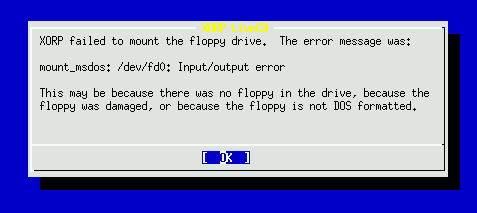
\includegraphics[width=6.0in]{figs/cd1}
    \caption{LiveCD missing floppy-related warning}
    \label{fig:livecd:cd1}
  \end{center}
\end{figure}

Hit enter, and you'll be given the choices shown in
Figure~\ref{fig:livecd:cd2}.

\begin{figure}[h]
  \begin{center}
    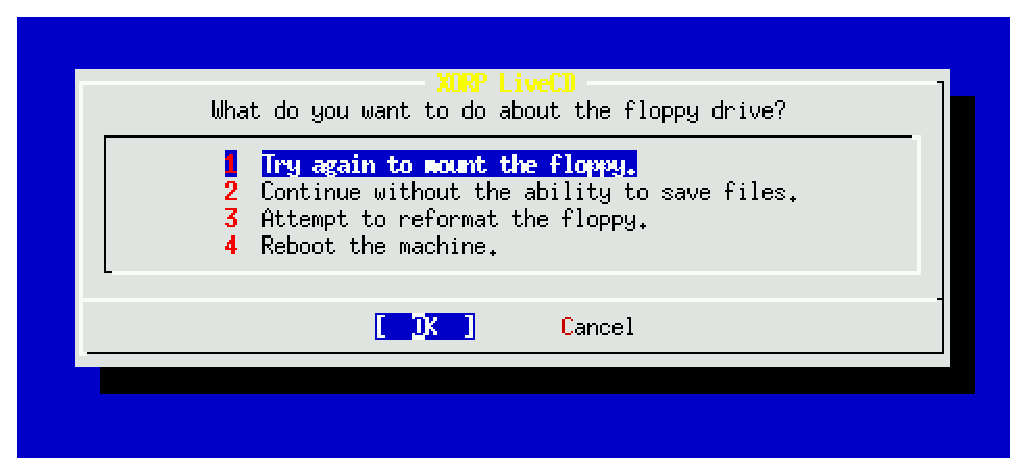
\includegraphics[width=6.0in]{figs/cd2}
    \caption{LiveCD floppy-related menu}
    \label{fig:livecd:cd2}
  \end{center}
\end{figure}


Use the cursor keys to move up and down to choose an option, and hit enter.

If you hadn't got a floppy in the drive, you can add one now, and select 1.

If your floppy is not DOS formatted, you can reformat it (erasing all the data
on it) by selecting 3.

If you don't have a floppy to hand, you can continue by selecting 2,
but you won't be able to preserve any configuration changes you make
later.

If you now have a blank writable DOS formatted floppy in the floppy
drive, you'll get the notice shown in Figure~\ref{fig:livecd:cd3}.

\begin{figure}[h]
  \begin{center}
    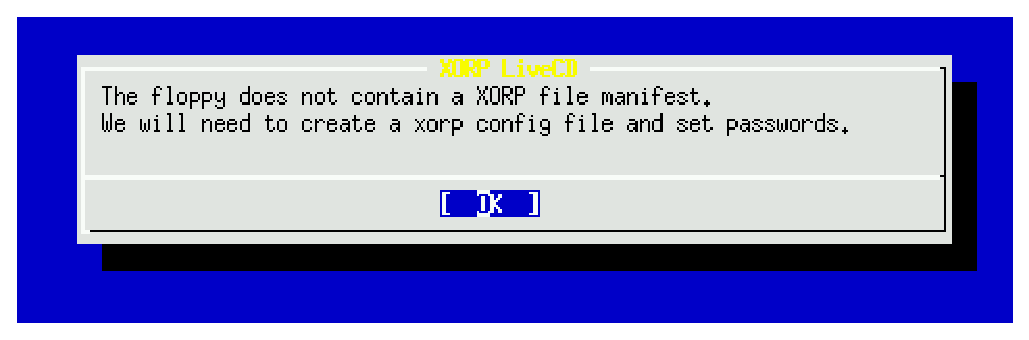
\includegraphics[width=6.0in]{figs/cd3}
    \caption{LiveCD floppy-related message}
    \label{fig:livecd:cd3}
  \end{center}
\end{figure}

Hit Enter, and you will be prompted to enter the root password for the
FreeBSD system.  This will allow you to login to the machine as the
superuser to diagnose any problems, or to see how XORP works behind
the scenes.

Next you will be prompted to enter the password for the "xorp" user
account.  On a normal XORP router, you might have many user accounts
for the different router administrators, but on the Live CD we just
create one user called "xorp".  Please do enter a reasonable password,
as this user will be able to login over the network using the ssh
secure shell and this password.

Finally you will be prompted as to which network interfaces you wish
XORP to manage.  These interfaces will show up in the default XORP
configuration file, ready to have IP addresses assigned.  The menu
looks like the one shown in Figure~\ref{fig:livecd:cd4}.

\begin{figure}[h]
  \begin{center}
    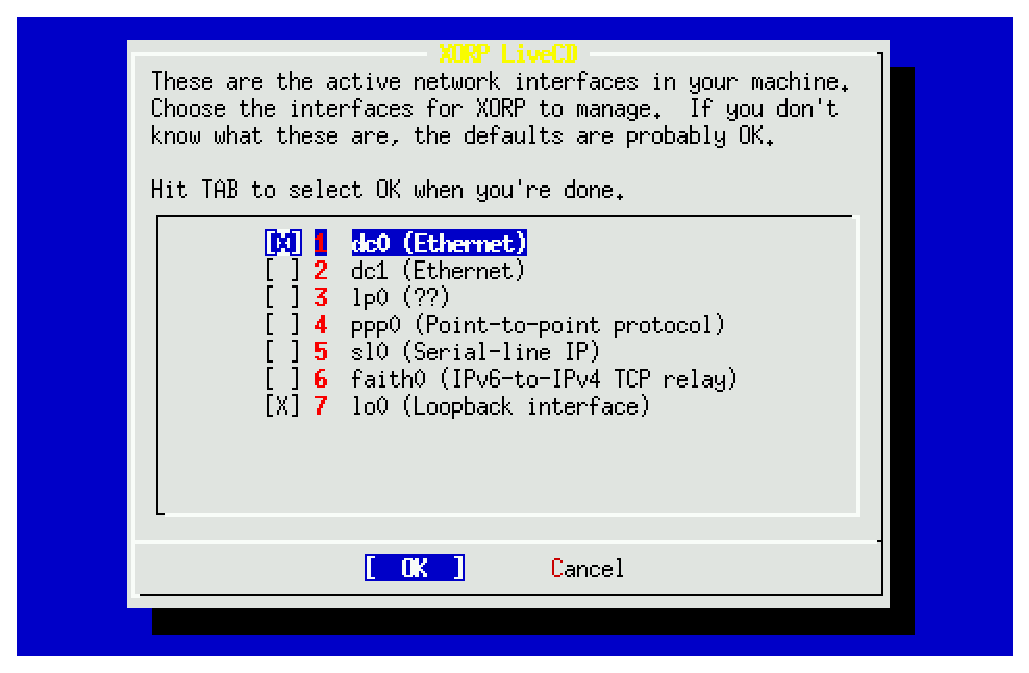
\includegraphics[width=6.0in]{figs/cd4}
    \caption{LiveCD network interfaces menu}
    \label{fig:livecd:cd4}
  \end{center}
\end{figure}

Typically you will only want XORP to manage Ethernet interfaces and
the loopback interface from the Live CD at this stage, because currently
XORP has no built-in support for dial-up links.  Move up and down using the
cursor keys, and hit space to select or unselect an option (an "X"
implies the option is selected).  When you are finished, hit Tab, to
select the "OK" button, and hit Enter.

That's it.  XORP will now finish booting.

Once XORP has finished booting, you will be presented with a login
prompt, and you can login to XORP as the "xorp" user with the password
you have chosen, and interact with the XORP command line interface to
complete the configuration, assign IP addresses, etc.

\section{Saving Config}

The location of the router configuration file used by XORP can be set
using command line parameters, so different XORP systems might choose
to use a different location for this file.  On the Live CD, the
configuration file is stored in {\stt /etc/xorp.cfg}.

If you change the router configuration using the XORP shell, and want
to save it, you need to enter the following in configuration mode:

\vspace{0.1in}
\noindent\framebox[\textwidth][l]{\scriptsize
\begin{minipage}{6in}
\begin{alltt}
\begin{tabbing}
xxxxxxxxxxxxxxxxxx\=\kill
user@hostname\# \textbf{save /etc/xorp.cfg}
\end{tabbing}
\end{alltt}
\end{minipage}
}
\vspace{0.1in}

If you save to any other location, the file will still be preserved on
the floppy, but will not be loaded automatically the next time XORP reboots.

\section{Debugging}

The Live CD includes two versions of the XORP system binaries.  The
normal version is mounted in a memory filesystem in
{\stt /usr/local/xorp</B>}.  This version has had the debugging systems
stripped so that the binaries are small enough to reside in a memory
filesystem.  This allows them to load quickly, and to run on a PC with
less memory.

If you need a debugging version, you can run the following command:

{\tt umount /usr/local/xorp}

A second copy of {\stt /usr/local/xorp} with debugging
binaries resides on the CD, and is revealed when the memory filesystem
is unmounted.  These binaries are rather large, and load slowly, so
don't use them unless you really need them.  Using them rather assumes
you know how XORP works internally, so is beyond the scope of this
tutorial.

\section{Interface Naming}

If you're used to Linux, you may be surprised that FreeBSD names it's
Ethernet interfaces with names like {\stt fxp0}, {\stt fxp1},
{\stt dc0} and {\stt xl3}, rather than {\stt eth0}, {\stt eth1}, etc.
The advantage is that you can tell exactly what the device driver is
that's being used, and that if you know you have one Intel 10/100 and one
DEC Tulip in the machine, you know they'll be called {\stt fxp0} and
{\stt dc0}, no matter which PCI slot they're in.  The disadvantage is
that it's more confusing for beginners who don't want to know this detail.

Some people get religious about such things.  We don't - this just
reflects the underlying operating system's naming convention.  If you
ran XORP on Linux, you'd see {\stt eth0}, etc.


%%%%%%%%%%%%%%%%%%%%%%%%%%%%%%%%%%%%%%%%%%%%%%%%%%%%%%%%%%%%%%%%%%%%%%%
%     BIBLIOGRAPHY
%%%%%%%%%%%%%%%%%%%%%%%%%%%%%%%%%%%%%%%%%%%%%%%%%%%%%%%%%%%%%%%%%%%%%%%
\bibliography{../tex/xorp}
\bibliographystyle{plain}

%%%%%%%%%%%%%%%%%%%%%%%%%%%%%%%%%%%%%%%%%%%%%%%%%%%%%%%%%%%%%%%%%%%%%%%
\end{document}
